% AAU_P5_report
%--------------------------------------------------------------%
%  A simple AAU report template.
%  2015-05-08 v. 1.2.0
%  Copyright 2010-2015 by Jesper Kjær Nielsen <jkn@es.aau.dk>
%
%  This is free software: you can redistribute it and/or modify
%  it under the terms of the GNU General Public License as published by
%  the Free Software Foundation, either version 3 of the License, or
%  (at your option) any later version.
%
%  This is distributed in the hope that it will be useful,
%  but WITHOUT ANY WARRANTY; without even the implied warranty of
%  MERCHANTABILITY or FITNESS FOR A PARTICULAR PURPOSE.  See the
%  GNU General Public License for more details.
%
%  You can find the GNU General Public License at <http://www.gnu.org/licenses/>.
%
\documentclass[11pt,twoside,a4paper,openright]{report}
%%%%%%%%%%%%%%%%%%%%%%%%%%%%%%%%%%%%%%%%%%%%%%%%
% Language, Encoding and Fonts
% http://en.wikibooks.org/wiki/LaTeX/Internationalization
%%%%%%%%%%%%%%%%%%%%%%%%%%%%%%%%%%%%%%%%%%%%%%%%
% Select encoding of your inputs. Depends on
% your operating system and its default input
% encoding. Typically, you should use
%   Linux  : utf8 (most modern Linux distributions)
%            latin1 
%   Windows: ansinew
%            latin1 (works in most cases)
%   Mac    : applemac
% Notice that you can manually change the input
% encoding of your files by selecting "save as"
% an select the desired input encoding. 
\usepackage[utf8]{inputenc}

%code formating 
\usepackage{listings}
\usepackage{adjustbox}
\usepackage{float}
\usepackage{color}
%graphs


% Make latex understand and use the typographic
% rules of the language used in the document.
\usepackage[danish,english]{babel}
% Use the palatino font
\usepackage[sc]{mathpazo}
\linespread{1.05}         % Palatino needs more leading (space between lines)
% Choose the font encoding
\usepackage[T1]{fontenc}
%%%%%%%%%%%%%%%%%%%%%%%%%%%%%%%%%%%%%%%%%%%%%%%%
% Graphics and Tables
% http://en.wikibooks.org/wiki/LaTeX/Importing_Graphics
% http://en.wikibooks.org/wiki/LaTeX/Tables
% http://en.wikibooks.org/wiki/LaTeX/Colors
%%%%%%%%%%%%%%%%%%%%%%%%%%%%%%%%%%%%%%%%%%%%%%%%
% load a colour package
\usepackage{xcolor}
\definecolor{aaublue}{RGB}{33,26,82}% dark blue
% The standard graphics inclusion package
\usepackage{graphicx}
\graphicspath{ {figures/} }
\DeclareGraphicsExtensions{.png,.pdf}
% Set up how figure and table captions are displayed
\usepackage{caption}
\captionsetup{%
  font=footnotesize,% set font size to footnotesize
  labelfont=bf % bold label (e.g., Figure 3.2) font
}
% Make the standard latex tables look so much better
\usepackage{array,booktabs}
% Enable the use of frames around, e.g., theorems
% The framed package is used in the example environment
\usepackage{framed}

%%%%%%%%%%%%%%%%%%%%%%%%%%%%%%%%%%%%%%%%%%%%%%%%
% Mathematics
% http://en.wikibooks.org/wiki/LaTeX/Mathematics
%%%%%%%%%%%%%%%%%%%%%%%%%%%%%%%%%%%%%%%%%%%%%%%%
% Defines new environments such as equation,
% align and split 
\usepackage{amsmath}
% Adds new math symbols
\usepackage{amssymb}
% Use theorems in your document
% The ntheorem package is also used for the example environment
% When using thmmarks, amsmath must be an option as well. Otherwise \eqref doesn't work anymore.
\usepackage[framed,amsmath,thmmarks]{ntheorem}

%%%%%%%%%%%%%%%%%%%%%%%%%%%%%%%%%%%%%%%%%%%%%%%%
% Page Layout
% http://en.wikibooks.org/wiki/LaTeX/Page_Layout
%%%%%%%%%%%%%%%%%%%%%%%%%%%%%%%%%%%%%%%%%%%%%%%%
% Change margins, papersize, etc of the document
\usepackage[
  inner=28mm,% left margin on an odd page
  outer=41mm,% right margin on an odd page
  ]{geometry}
% Modify how \chapter, \section, etc. look
% The titlesec package is very configureable
\usepackage{titlesec}
\titleformat{\chapter}[display]{\normalfont\huge\bfseries}{\chaptertitlename\ \thechapter}{20pt}{\Huge}
\titleformat*{\section}{\normalfont\Large\bfseries}
\titleformat*{\subsection}{\normalfont\large\bfseries}
\titleformat*{\subsubsection}{\normalfont\normalsize\bfseries}
%\titleformat*{\paragraph}{\normalfont\normalsize\bfseries}
%\titleformat*{\subparagraph}{\normalfont\normalsize\bfseries}

% Clear empty pages between chapters
\let\origdoublepage\cleardoublepage
\newcommand{\clearemptydoublepage}{%
  \clearpage
  {\pagestyle{empty}\origdoublepage}%
}
\let\cleardoublepage\clearemptydoublepage

% Change the headers and footers
\usepackage{fancyhdr}
\pagestyle{fancy}
\fancyhf{} %delete everything
\renewcommand{\headrulewidth}{0pt} %remove the horizontal line in the header
\fancyhead[RE]{\small\nouppercase\leftmark} %even page - chapter title
\fancyhead[LO]{\small\nouppercase\rightmark} %uneven page - section title
\fancyhead[LE,RO]{\thepage} %page number on all pages
% Do not stretch the content of a page. Instead,
% insert white space at the bottom of the page
\raggedbottom
% Enable arithmetics with length. Useful when
% typesetting the layout.
\usepackage{calc}

%%%%%%%%%%%%%%%%%%%%%%%%%%%%%%%%%%%%%%%%%%%%%%%%
% Bibliography
% http://en.wikibooks.org/wiki/LaTeX/Bibliography_Management
%%%%%%%%%%%%%%%%%%%%%%%%%%%%%%%%%%%%%%%%%%%%%%%%
\usepackage[backend=biber,
bibencoding=utf8, sorting=none]{biblatex}
\addbibresource{bib/mybib}
\usepackage{csquotes}

%%%%%%%%%%%%%%%%%%%%%%%%%%%%%%%%%%%%%%%%%%%%%%%%
% Misc
%%%%%%%%%%%%%%%%%%%%%%%%%%%%%%%%%%%%%%%%%%%%%%%%
% Add bibliography and index to the table of
% contents
\usepackage[nottoc]{tocbibind}
% Add the command \pageref{LastPage} which refers to the
% page number of the last page
\usepackage{lastpage}
% Add todo notes in the margin of the document
\usepackage[
%  disable, %turn off todonotes
  colorinlistoftodos, %enable a coloured square in the list of todos
  textwidth=\marginparwidth, %set the width of the todonotes
  textsize=scriptsize, %size of the text in the todonotes
  ]{todonotes}

%%%%%%%%%%%%%%%%%%%%%%%%%%%%%%%%%%%%%%%%%%%%%%%%
% Hyperlinks
% http://en.wikibooks.org/wiki/LaTeX/Hyperlinks
%%%%%%%%%%%%%%%%%%%%%%%%%%%%%%%%%%%%%%%%%%%%%%%%
% Enable hyperlinks and insert info into the pdf
% file. Hypperref should be loaded as one of the 
% last packages
\usepackage{hyperref}
\hypersetup{%
	pdfpagelabels=true,%
	plainpages=false,%
	pdfauthor={Author(s)},%
	pdftitle={Title},%
	pdfsubject={Subject},%
	bookmarksnumbered=true,%
	colorlinks=false,%
	citecolor=black,%
	filecolor=black,%
	linkcolor=black,% you should probably change this to black before printing
	urlcolor=black,%
	pdfstartview=FitH%
}
% package inclusion and set up of the document
% see, e.g., http://en.wikibooks.org/wiki/LaTeX/Formatting#Hyphenation
% for more information on word hyphenation
\hyphenation{ex-am-ple hy-phen-a-tion short}
\hyphenation{long la-tex}
% 
%  A simple AAU report template.
%  2015-05-08 v. 1.2.0
%  Copyright 2010-2015 by Jesper Kjær Nielsen <jkn@es.aau.dk>
%
%  This is free software: you can redistribute it and/or modify
%  it under the terms of the GNU General Public License as published by
%  the Free Software Foundation, either version 3 of the License, or
%  (at your option) any later version.
%
%  This is distributed in the hope that it will be useful,
%  but WITHOUT ANY WARRANTY; without even the implied warranty of
%  MERCHANTABILITY or FITNESS FOR A PARTICULAR PURPOSE.  See the
%  GNU General Public License for more details.
%
%  You can find the GNU General Public License at <http://www.gnu.org/licenses/>.
%
%
%
% see, e.g., http://en.wikibooks.org/wiki/LaTeX/Customizing_LaTeX#New_commands
% for more information on how to create macros

%%%%%%%%%%%%%%%%%%%%%%%%%%%%%%%%%%%%%%%%%%%%%%%%
% Macros for the titlepage
%%%%%%%%%%%%%%%%%%%%%%%%%%%%%%%%%%%%%%%%%%%%%%%%
%Creates the aau titlepage
\newcommand{\aautitlepage}[3]{%
  {
    %set up various length
    \ifx\titlepageleftcolumnwidth\undefined
      \newlength{\titlepageleftcolumnwidth}
      \newlength{\titlepagerightcolumnwidth}
    \fi
    \setlength{\titlepageleftcolumnwidth}{0.5\textwidth-\tabcolsep}
    \setlength{\titlepagerightcolumnwidth}{\textwidth-2\tabcolsep-\titlepageleftcolumnwidth}
    %create title page
    \thispagestyle{empty}
    \noindent%
    \begin{tabular}{@{}ll@{}}
      \parbox{\titlepageleftcolumnwidth}{
        \iflanguage{danish}{%
          
\includegraphics[width=\titlepageleftcolumnwidth]{figures/aau_logo_da}
        }{%
          
\includegraphics[width=\titlepageleftcolumnwidth]{figures/aau_logo_en}
        }
      } &
      \parbox{\titlepagerightcolumnwidth}{\raggedleft\sf\small
        #2
      }\bigskip\\
       #1 &
      \parbox[t]{\titlepagerightcolumnwidth}{%
      \textbf{Abstract:}\bigskip\par
        \fbox{\parbox{\titlepagerightcolumnwidth-2\fboxsep-2\fboxrule}{%
          #3
        }}
      }\\
    \end{tabular}
    \vfill
    \iflanguage{danish}{%
      \noindent{\footnotesize\emph{Rapportens indhold er frit tilgængeligt, men offentliggørelse (med kildeangivelse) må kun ske efter aftale med forfatterne.}}
    }{%
      \noindent{\footnotesize\emph{Keywords: TensorFlow, Distributed Speech Recognition System, Artificial Neural Networks, Long-Short Term Memory RNN, Mel-Frequency Cepstral Coefficients, Data Mining}}
    }
    \clearpage
  }
}

%Create english project info
\newcommand{\englishprojectinfo}[8]{%
  \parbox[t]{\titlepageleftcolumnwidth}{
    \textbf{Title:}\\ #1\bigskip\par
    \textbf{Theme:}\\ #2\bigskip\par
    \textbf{Project Period:}\\ #3\bigskip\par
    \textbf{Project Group:}\\ #4\bigskip\par
    \textbf{Participant(s):}\\ #5\bigskip\par
    \textbf{Supervisor(s):}\\ #6\bigskip\par
    \textbf{Copies:} #7\bigskip\par
    \textbf{Page Numbers:} \pageref{LastPage}\bigskip\par
    \textbf{Date of Completion:}\\ #8
  }
}

%%%%%%%%%%%%%%%%%%%%%%%%%%%%%%%%%%%%%%%%%%%%%%%%
% An example environment
%%%%%%%%%%%%%%%%%%%%%%%%%%%%%%%%%%%%%%%%%%%%%%%%
\theoremheaderfont{\normalfont\bfseries}
\theorembodyfont{\normalfont}
\theoremstyle{break}
\def\theoremframecommand{{\color{gray!50}\vrule width 5pt \hspace{5pt}}}
\newshadedtheorem{exa}{Example}[chapter]
\newenvironment{example}[1]{%
		\begin{exa}[#1]
}{%
		\end{exa}
}
% my new macros

%--------------------------------------------------------------%
\begin{document}
	%frontmatter
	\pagestyle{empty} %disable headers and footers
	\pagenumbering{roman} %use roman page numbering in the frontmatter
	
	%  A simple AAU report template.
%  2015-05-08 v. 1.2.0
%  Copyright 2010-2015 by Jesper Kjær Nielsen <jkn@es.aau.dk>
%
%  This is free software: you can redistribute it and/or modify
%  it under the terms of the GNU General Public License as published by
%  the Free Software Foundation, either version 3 of the License, or
%  (at your option) any later version.
%
%  This is distributed in the hope that it will be useful,
%  but WITHOUT ANY WARRANTY; without even the implied warranty of
%  MERCHANTABILITY or FITNESS FOR A PARTICULAR PURPOSE.  See the
%  GNU General Public License for more details.
%
%  You can find the GNU General Public License at <http://www.gnu.org/licenses/>.
%
\pdfbookmark[0]{Front page}{label:frontpage}%
\begin{titlepage}
  \addtolength{\hoffset}{0.5\evensidemargin-0.5\oddsidemargin} %set equal margins on the frontpage - remove this line if you want default margins
  \noindent%
  \begin{tabular}{@{}p{\textwidth}@{}}
    \toprule[2pt]
    \midrule
    \vspace{0.2cm}
    \begin{center}
    \Huge{\textbf{
      Report Title% insert your title here
    }}
    \end{center}
    \begin{center}
      \Large{
        - Subtitle -% insert your subtitle here
      }
    \end{center}
    \vspace{0.2cm}\\
    \midrule
    \toprule[2pt]
  \end{tabular}
  \vspace{4 cm}
  \begin{center}
    {\large
      Project Report%Insert document type (e.g., Project Report)
    }\\
    \vspace{0.2cm}
    {\Large
      Group Name/Number%Insert your group name or real names here
    }
  \end{center}
  \vfill
  \begin{center}
  Aalborg University\\
  Electronics and IT
  \end{center}
\end{titlepage}
\clearpage

	\thispagestyle{empty}
{\small
\strut\vfill % push the content to the bottom of the page
\noindent Copyright \copyright{} Aalborg University 2017\par
\vspace{0.2cm}

}
\clearpage
\todo{}


	\pdfbookmark[0]{English title page}{label:titlepage_en}
\aautitlepage{%
  \englishprojectinfo{
    Speech Recognition %title
  }{%
    Scientific Theme %theme
  }{%
    Fall Semester 2017 %project period
  }{%
    ED5-1-E17 % project group
  }{%
    %list of group members
    Stefan Bîrs\\
    Tiberiu-Ioan Szatmari\\
    Kamran Thomas Alimagham
    
  }{%
    %list of supervisors
    Daniel Ortiz-Arroyo\\
    D. M. Akbar Hussain
  }{%
    1 % number of printed copies
  }{%
    \today % date of completion
  }%
}{%department and address
  \textbf{Electronics and IT}\\
  Aalborg University\\
  \href{http://www.aau.dk}{http://www.aau.dk}
}{% the abstract
  This report goes into detail about the implementation         
  of distributed speech recognition systems, information  
  retrieval and machine learning. A historical overview
  is presented to display the different methods
  for achieving a practical model for speech recognition. The main part
  of the project was based around machine learning and neural
  networks so the report includes explanations of the fundamental principles
  used.It encapsulates the entire process that was required to achieve a fully
  operational system. A .flac to .wav file conversion algorithm was developed
   and used to create newer and larger data sets used for training. The
   Mel Frequency Cepstrum was used as a filter and pre-processing technique. All
   of the above mentioned steps were used to pursue a bidirectional, deep 
   recurrent network which uses complex LSTM layers.
   
}
\cleardoublepage

	\cleardoublepage
	\pdfbookmark[0]{Contents}{label:contents}
	\pagestyle{fancy} %enable headers and footers again
	\tableofcontents
	\listoftodos
	
	\chapter*{Preface\markboth{Preface}{Preface}}\label{ch:preface}
\addcontentsline{toc}{chapter}{Preface}
The project entitled Speech Recognition with Focus
on information retrieval and command prompt was made by three students from the Electronics and Computer Engineering programme at Aalborg University Esbjerg, for the P5 project during the fifth semester.

\vspace{\baselineskip}\hfill Aalborg University, \today
\vfill\noindent
\begin{minipage}[b]{0.45\textwidth}
 \centering
 \rule{\textwidth}{0.5pt}\\
  Stefan Bîrs\\
 {\footnotesize <sbars15@student.aau.dk>}
\end{minipage}
\hfill
\begin{minipage}[b]{0.45\textwidth}
 \centering
 \rule{\textwidth}{0.5pt}\\
  Tiberiu-Ioan Szatmari\\
 {\footnotesize <tszatm15@student.aau.dk>}
\end{minipage}
\vspace{3\baselineskip}
\begin{center}
\begin{minipage}[b]{0.45\textwidth}
 \centering
 \rule{\textwidth}{0.5pt}
  Kamran Thomas Alimagham\\
 {\footnotesize <kalima15@student.aau.dk>}
\end{minipage}
\end{center}

	\cleardoublepage
	%mainmatter
	\pagenumbering{arabic} %use arabic page numbering in the mainmatter
	%---------------------------------------------------------%
	\chapter{Introduction}\label{ch:introduction}
The focus of this project will be on implementing a distributed speech recognition (DSR) system.
The main focus is to understand, design and implement an artificial neural network that can recognize human speech using deep learning methods.
The toolkit that we will use for the machine learning part was developed by the Google Brain Team and it`s now an open-source, software library, called TensorFlow (TF) \cite{tensorflow2015-whitepaper}.
At the time of this project, the newest update available is version 1.3.0.\\\\
Speech is probably the most important forms of communication.
It is the most natural and efficient way to communicate with
each other. Humans learn all the relevant skills during early
childhood, without any instruction, and they continue to rely
on speech communication throughout their life \cite{kamblespeech}.
Humans also want to have a similar, natural and efficient form of communication with machines. 
Until recently, the idea of holding a conversation with a computer seemed pure science fiction.\\\\
However, the situation is changing, and quickly.
A growing number of people now talk to their smartphones, asking them to set reminders, search for directions, or send email and text messages.
Chief technology officer of \copyright{} Nuance Communications, Vlad Sejnoha stated: "We`re at a transition point where voice and natural-language understanding are suddenly at the forefront" \cite{kamblespeech}.\\

\subsubsection{Reading guide}
In Chapter \ref{ch:speech_processing} the preprocessing part of the project is covered. In it, detailed explanations of historical and modern approaches are taken into consideration. Chapter \ref{ch:machine_learning} presents an introduction to the field of artificial neural networks and displays the learning process by gradually introducing more complex types of networks. Alongside the theoretical part, a practical introduction to TensorFlow is given in Chapter\ref{ch:machine_learning_platform}. Chapter \ref{ch:model_development} shows the difference between three working models, detailing the advantage of a bidirectional network model. Chapter \ref{ch:Network Framework} talks about the assembly and implementation of the distributed system. Chapter \ref{ch:implementation} and \ref{ch:discussion} provide a summary of the findings from the project, an analysis of future work and a closing argument. All the code and scripts used for the project can be found on the GitHub repository referenced here: \cite{mavericks2017}.

	
	\chapter{Problem Description}\label{ch:problem_description}
%---------------------------------------------------------
\section{Problem Description}

As mentioned above, the final goal for this project is to develop a distributed speech recognition (DSR) system.
In order to achieve this goal we need to gain a fundamental understanding in the field of machine learning and computer networks.\\

%---------------------------------------------------------
\section{Tools}
The following information is a selection of the relevant software and hardware tools used to implement the Graphics Processing Unit (GPU) accelerated training:

\subsubsection{Software Tools}
\begin{itemize}
	\item TensorFlow 1.3.0
	\item Visual Studio 2015
	\item cuDNN 8.0
	\item Python 3.6
	\item Linux ubuntu
	\item MATLAB  R2017b
\end{itemize}

\subsubsection{Hardware Tools}
\begin{itemize}
	\item Intel Computer
	\item Nvidia Geforce GTX 1070 \\
\end{itemize}

\subsubsection{Setup}

The GPU used in this project was a Nvidia GTX 1070 card with 1920 CUDA cores, a standard Memory Configuration of 8 GB GDDR5 and a maximum power consumption of $150W$ \cite{GPU}. It was added to a computer with an Intel Core I7-4770 CPU and 8 GB of RAM memory. The operating system was Windows 7 Enterprise.


%---------------------------------------------------------
\section{Problem Delimitation}\label{sec:PD}
To ensure that the project meets the desired scope,
specific success criteria are formed which will be
evaluated during the final stages of the report.
The following list of requirements are the desired
success criteria, where the focus will be on reaching
the given goals:
\begin{itemize}
	\item Data mining
	\item Choose a filter
	\item Design a deep neural network model
	\item Train for the English language
	\item Create a Client/Server framework
	\item Implement the distributed model
\end{itemize}
A key component of neural networks is data. To increase their performance, using a large data set is necessary. As open-source, compatible, training data sets are hard to come by, data mining algorithms are created. This will allow the available data to fit the needs of the developed model.\\\\
Any real life sequence of recorded speech has some amount of noise, making it harder for the neural network to understand spoken words.
This can lead to errors that alter the word beyond recognition. 
To ameliorate this problem, a filter that mimics the human
ear is the best fit for such a project.\\\\
Along the report, a historical analysis of different knowledge
based solutions to the recognition of human speech is made.
By studying the existing literature and comparing open-source projects, a neural network can be built, with the scope of reducing the error rate and training time as much
as possible.\\\\
A Client/Server set-up allows for running different parts of the DSR system, on multiple, internet connected machines. This allows for the more demanding tasks to be processed remotely, minimizing the impact for the end-user.

%---------------------------------------------------------
	
	\chapter{Speech Processing}\label{ch:speech_processing}
Speech is an effortless and highly efficient form of communication.
Continuous speech recognition software is readily available from stores and it allows the user to interact with its surrounding without the need of written commands
\cite[p.~396]{callan2003artificial}. Amazon`s Alexa 
\cite{Alexa} and Microsoft`s Cortana 
\cite{Cortana} are perfect examples of home companions that are able to perform basic tasks received via voice commands.\\\\
As speech recognition increases in accuracy, this technology will make the leap from being annoying to use, to becoming the main way we interact with computers. 
This idea is further backed up by the fact that people tend to speak much faster than they are able to type \cite{Speed}.
In some cases, speech can be three times faster in conveying information than typing, and for professional debaters,
speaking can be even six times faster.
\todo{We looked over until here...}

\section{Classical overview}
Words are carried as sound waves, which are analogue signals.
In order for speech to be processed,
it needs to be run through a signal processor that selects the frequencies and amplitude of the signal.
Further on, the signal is mapped to individual sound units called phones.
These phones need to be identified and grouped in such a way to ensure that each word has a different phonetic structure,
otherwise, words would be impossible to distinguish from one another.
\begin{table}[H]
\centering
	\caption{Phones.}
	\label{my-label}
	\begin{tabular}{l l}
		{[}ay{]} & \underline{ir}is \\
		{[}b{]}  & \underline{b}in  \\
		{[}er{]} & \underline{bir}d \\
		{[}l{]}  & \underline{l}ip  \\
		{[}p{]}  & \underline{p}in  \\
		{[}th{]} & \underline{thi}n
	\end{tabular}
\end{table}
Phones can have different sounds depending on the context. 
For example, the phone \textbf{th} in the word \textit{three} has a different sound to \textbf{th} in \textit{then}. 
To overcome these different variations of the same phones, 
it is better to abstract the phones into a generalized grouping called a \textbf{phoneme}.
Phonemes are written in-between forward slashes
(\textit{/th/}) and they will have a specific pronunciation for each sound, depending on the context.
These phonemes are used as a transitional layer when trying to convert speech to text and vice versa,
when speech needs to be synthesized.

\section{Signal processing}
Sound waves that carry human speech are variations in air pressure.
The key components of a sound wave are its \textbf{amplitude},
which measure the intensity of the sound and the \textbf{frequency}, which describes the rate at which the amplitude varies over time.
When speaking in a microphone,
the change in air pressure causes the diaphragm to oscillate.
The size of the oscillations is directly proportional to the amplitude of the signal,
while the rate at which the diaphragm oscillates represents the rate at which the air pressure changes.
At specific time intervals,
the signal can be sampled and the data can be used in a wide array of digital signal processing tools.
For example, the digital signal can be plotted as a two dimensional plot,
where the y-axis defines the amplitude and the x-axis shows the time.
The frequency can be easily be determined from the plot as the number of cycles that the signal does per second.\\\\
Although a visual difference can be seen when plotting vowels and consonants,
a visual inspection of the waveform will not reveal any critical information, making it impossible to see all the phonemes.\\\\
To feed this information to the neural network, some preprocessing and signal manipulation is required so the input can be understood and passed through the neurons.
These steps are expanded upon in the following subsections.

\subsubsection{ Preprocessing}
No matter how powerful and how advanced a computer is,
it still works in discrete time.
In order to represent an analogue signal on the computer, it has to be sampled according to the Nyquist sampling theorem.
This theorem states that the sampling frequency has to be at least double the frequency of the original signal in order to replicate the original signal without aliasing.
For a better understanding of the process, a visual representation of the word "Hello" as it is formed for the input of the neural network is shown in the upper part of Figure \ref{fig:cyka}.

\subsubsection{ Fourier transform}
To analyse a discrete signal we use the Fourier transform. 
This allows us to convert the signal in the frequency domain and deconstruct it in a series of simple sine waves. 
These sine waves have specific amplitudes and frequencies and while plotting the FFT of the signal, 
the dominant waves can be identified by the intensity of the amplitude.\\\\
In the lower part of Figure \ref{fig:cyka}, a visual representation of the FFT is shown. 
It can be seen that there are a lot of frequencies that make up the word "Hello". 
The dominant ones are in the range of $500 Hz$. 
Considering that this recording has a minimum amount of noise,
we have to consider the full range of the frequencies,
from zero and up to 3500 Hz.
\begin{figure}[H]
	\centering
	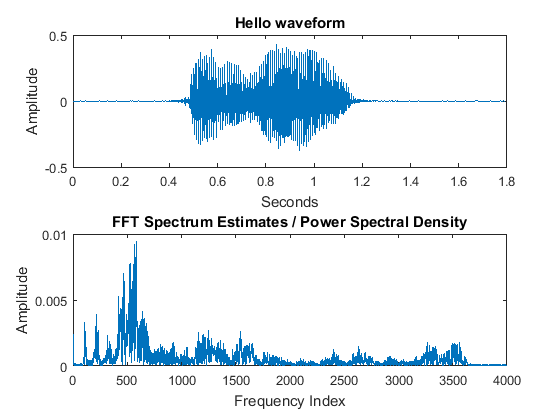
\includegraphics[width=0.75\textwidth]		
	{speech_processing/03_FFTpluswaveform}
	\caption{Waveform and FFT computed for the word "Hello".}
	\label{fig:cyka}
\end{figure}

\subsubsection{Spectrogram}
The spectrogram of the signal was computed from the FFT and it shows a visual representation of the spectrum of frequencies marked by the intensity of the color.
After the spectrogram is sliced into 25 ms chunks, it is feed as the input to the network. 
A neural network can find patterns in this data more easily than raw sound waves because certain patterns can be distinguished in the graph. Such a spectrogram can be seen in Appendix \ref{ch:appAlabel}, Figure \ref{fig:Spectrogram}.

\section{Modern analysis}\label{sec:Modernanalysis}
In the last decade, the state-of-the-art speech recognition models were phonetic-based
 approaches. Acoustic models with generative probabilistic models for sequential 
data, like the Hidden Markov Model (HMM) require both text and speech data and,
furthermore a word to phoneme dictionary.
 Even though these models can be made more accurate when speech data is correlated with phoneme transcriptions, this is a gargantuan task to be attempted by hand. This makes 
 phoneme-level transcriptions less likely to be used on large data sets.
  Both  speech recognizers of the past and today  rely on segmenting sound waves, but word based processing is far more efficient in modern speech recognizer (SR) systems.
  
\subsubsection{Mel Frequency Cepstrum Coefficients}
Mel-frequency cepstral coefficients (MFCCs) are coefficients that collectively make up a Mel-frequency cepstral (MFC). 
They are taken from a cepstral representation of the audio clip by finding the spectrum of the spectrum of the original audio file.
 Compared to normal cepstrum, in MFC, the frequency bands are spaced at equal distances on the Mel scale.
 This mimics a humans response to sound better that a linearly represented frequency band \cite{sahidullah2012design}.\\\\
Speech is a continuous action, where the present utterance will affect the future one. Combined with the fact that the English language is not a phonetic language means that a direct
representation of each character to their sound is impossible. To overcome this problem, the neural network is trained on overlapping windows both before and after the current speech sample.\\\\
In the model developed by us, nine slices of audio are used before and after the current index, adding up to $19$ time points for each window. With $26$ cepstral coefficients, this gives $494$ data points per $25ms$ observation, sampled at $16 000 Hz$ and seen in Listing \ref{lst:MFCC}.\\\

\begin{lstlisting}[language = Python, flexiblecolumns=true, label=lst:MFCC, caption = Example code to obtain MFCC features.]
# Load wav files
fs, audio = wav.read(audio_filename)
 
# Get mfcc coefficients
orig_inputs = mfcc(audio, samplerate=fs, numcep=numcep)
 
# For each time slice of the training set, we need to copy the context this makes
train_inputs = np.array([], np.float32)
train_inputs.resize((orig_inputs.shape[0], numcep + 2 * numcep * numcontext))
 
for time_slice in range(train_inputs.shape[0]):
    # Pick up to numcontext time slices in the past,
    # And complete with empty mfcc features
    need_empty_past = max(0, ((time_slices[0] + numcontext) - time_slice))
    empty_source_past = list(empty_mfcc for empty_slots in range(need_empty_past))
    data_source_past = orig_inputs[max(0, time_slice - numcontext):time_slice]
    assert(len(empty_source_past) + len(data_source_past) == numcontext)
\end{lstlisting}
 
\subsection{Connectionist Temporal Classification loss function}
 Discarding the use of phonemes for neural networks can be done by switching to an
 objective function that computes predictions at the character-level transcription.\\\\
Connectionist Temporal Classification (CTC) provides probabilities for multiple sets, encapsulating all possible character-level transcriptions of the speech sample.
The network uses the objective function to choose the highest probability for a transcription and calculates the error rate. The error is generated by comparing the
predicted result to the absolute value of the transcript before updating the weights of the network during training \cite{Great}.\\\\
The character-level error used by the CTC loss function is different from the Levenshtein \cite{stratonovich1960conditional} word error distance that is used in traditional models. Considering that the scope of this project is limited to the English language, it is important to know
that the character versus error rate will be quite different, because English is a non-phonetic language. An in depth analysis of the CTC inner works can be found in \cite{CTC1} and \cite{CTC2}. 
	
	\chapter{Machine Learning for Speech}\label{ch:machine_learning}

\section{Historical Overview}
The following section will encapsulate different methods that 
can be used in the field of speech processing and recognition.
Starting with statistical models and mapping algorithms,
further leading to knowledge based systems that render greater
efficiency when large data sets are available.

\subsubsection{Hidden Markov Model}

The forward and backward recursions used in HMM  were created by
Ruslan L. Stratonovich in 1960
\cite{stratonovich1960conditional}.
It is the most successfully used pattern recognition technique
used for speech recognition.
In contrast to knowledge based approaches,
this model has a strong and secure mathematical foundation
where a mathematical model is signalized on the Markov Model
and a set of output distribution. Speech is divided into
smaller audible samples where each sample represents a state
in the Markov Model. By the probabilities of transition,
there will be a shift from on state to another
\cite[p.~2]{gaikwad2010review}\cite{togneri1990speech}.

\subsubsection{Dynamic Time Warping}

Dynamic Time Warping (DTW) is an algorithm that compares words with pre-given reference words.
 It measures the patterns between two sequences that will vary in time or speed.\cite{togneri1990speech}
 To output speech, the algorithm tries to alter the time variable of the unknown speech until it matches on of the reference words.

\subsubsection{Vector Quantization}

Vector Quantization (VQ) is used to map vectors from a big vector space to a finite region in space. It needs compact code-blocks for reference models and codebook searcher in place of more costly evaluation methods. Each word receives a VQ codebook that is based on repeated sequences of the word. The test data is evaluated on all codebooks and the automated speech recogniser picks the codebook with the lowest distance measured.\cite[p.~20-21]{togneri1990speech}


\section{Artificial Neural Networks}
%---------------------------------------------------
\subsection{What is an Artificial Neural Network?}
Artificial Neural Networks are nothing but a computerized representation of the human brain. 
They have the ability to acquire and maintain knowledge (information based) and can be defined as a set of processing units, represented by artificial neurons,
interlinked by a lot of interconnections
(artificial synapses) \cite[p.~5]{Silva2016}.\\\\
The human brain learns from its experiences, creating new neural pathways. These interconnected chains of neurons are stronger than others and can be modulated, or changed,
following learning or during behavioural modifications.
The strongness of a neural connection is given by a weighted value, called synaptic weights.

\subsection{Artificial Neuron}
The Artificial neuron is the processing unit of an artificial neural network, which is a simplified model of the biological neuron.
This model was inspired by the analysis of how a cell membrane of a neuron generates and propagates electrical impulses(Hodgkin and Huxley 1952) \cite[p.~11]{Silva2016}.
The purpose of artificial neurons is to simulate the basic function of biological ones,
which are typically comprised of four parts:

\begin{enumerate}
	\item Dendrites: Accept inputs
	\item Soma(Cell body): Process the inputs
	\item Axon: Turn the processed inputs into outputs
	\item Synapses: The electrochemical connections between neurons 
\end{enumerate}
The following figure illustrates the four main functions of a biological neuron, represented on the artificial one. 

The artificial neurons used in artificial neural networks are non-linear, usually providing continuous outputs,
and performing simple functions,
such as gathering signals available on their inputs,
assembling them according to their operational functions,
and producing a response considering their innate activation functions \cite[p.~11]{Silva2016}. 

\begin{figure}[H]
\centering
	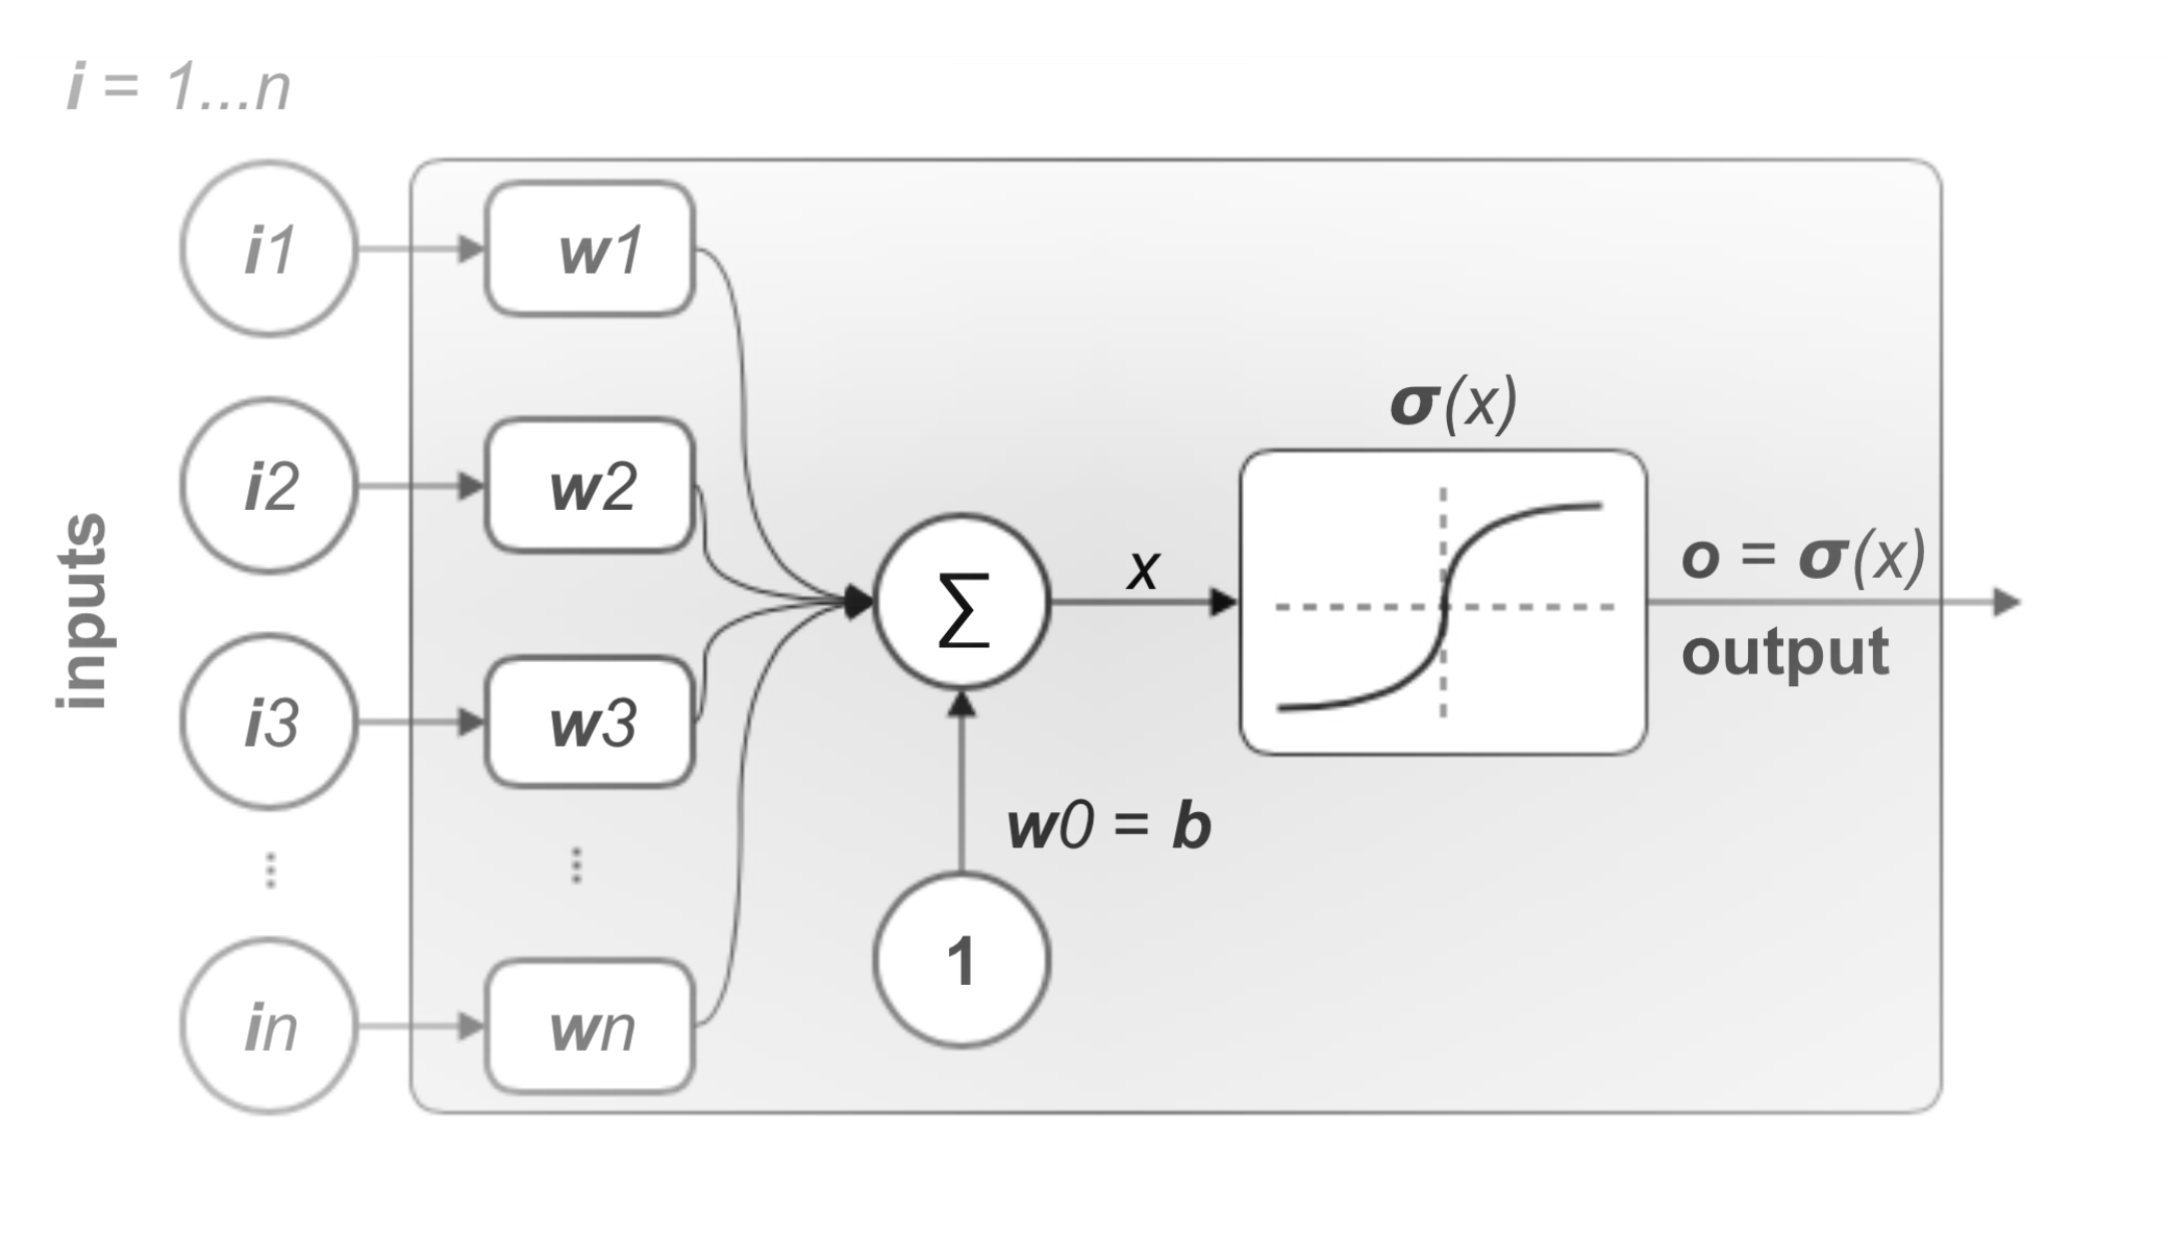
\includegraphics[width=\textwidth]
	{machine_learning/00_Artificial_Neuron}
	\caption{The artificial neuron.}
	\label{fig:AN}
\end{figure}

Each neuron from a network can be implemented as shown in Fig.
\ref{fig:AN}. The multiple input signals coming from the external environment are represented by the set
$\left\{i1,i2,i3,...,in \right\}$, analogous to the external electrical impulses gathered by the dendrites in the biological neuron.
\todo{re-write}

%---------------------------------------------------

\section{Types of Artificial Neural Networks}
%---------------------------------------------------
 
\subsection{Feed forward Network}


This type of simple neural network is comprised of one input
layer and one neural layer, which also acts as the output layer.
The flow of information is uni directional, starting from the input layer and progressing to the output layer. As such, the number of outputs from the neural network will always coincide with the number of neurons in the network.
 These networks are usually employed in
pattern classification and linear filtering problems. 
The Perceptron and the ADALINE architectures are among the most recognised feed-forward neural networks and they work well with Hebb`s rule and the Delta rule for training.

\subsection{Deep Recurrent Neural Network}
To explain how a deep recurrent neural network(RNN) looks like first we will see what a deep neural network is made of and after that the recurrent part will be added to form a more complex and and powerful network.

Networks with multiple layers are have one or more hidden neural layers. Such a network will always have one input layer with multiple samples and a series of variable layers.
In contrast to the simple feed-forward network, these hidden layers are not constrained to have the same size as the input layer. This means
that the size can depend on the complexity of the problem being
tackled by the network, as well as the quantity and quality of the available data. The last layer still occupies a double role as both a neuron layer and output layer.

Another key element is the fact that the outputs of the neurons  are used for feedback inputs to the other neurons.
This feature makes the network great for time-variant systems where the new outputs can benefit from previous information.

\subsection{Long Short Term Memory}
Long Short Term Memory networks, for short “LSTMs”, are a special case of recurrent neural network that  capable of learning long-term dependencies.
Firstly used in 1997 by Sepp Hochreiter and Jürgen Schmidhuber \cite{Father} and refined by Felix Gers and his team \cite{Gers99}.
Nowadays, after further refinement,
LSTMs work incredibly well on various problems and give better results for most problems that require RNNs.
They remember information for long periods of time by default, making them the perfect fit to avoid long-term dependency problems. 

LSTMs have a chain like structure of four layers, with repeating modules that interact in  specific ways. For simplicity, in the following explanation of the internal states of a LSTM, the input X will represent the normal input to the network concatenated with the previous state, $X = x_i | h_{t-1}$.

\begin{figure}[H]
	\centering
	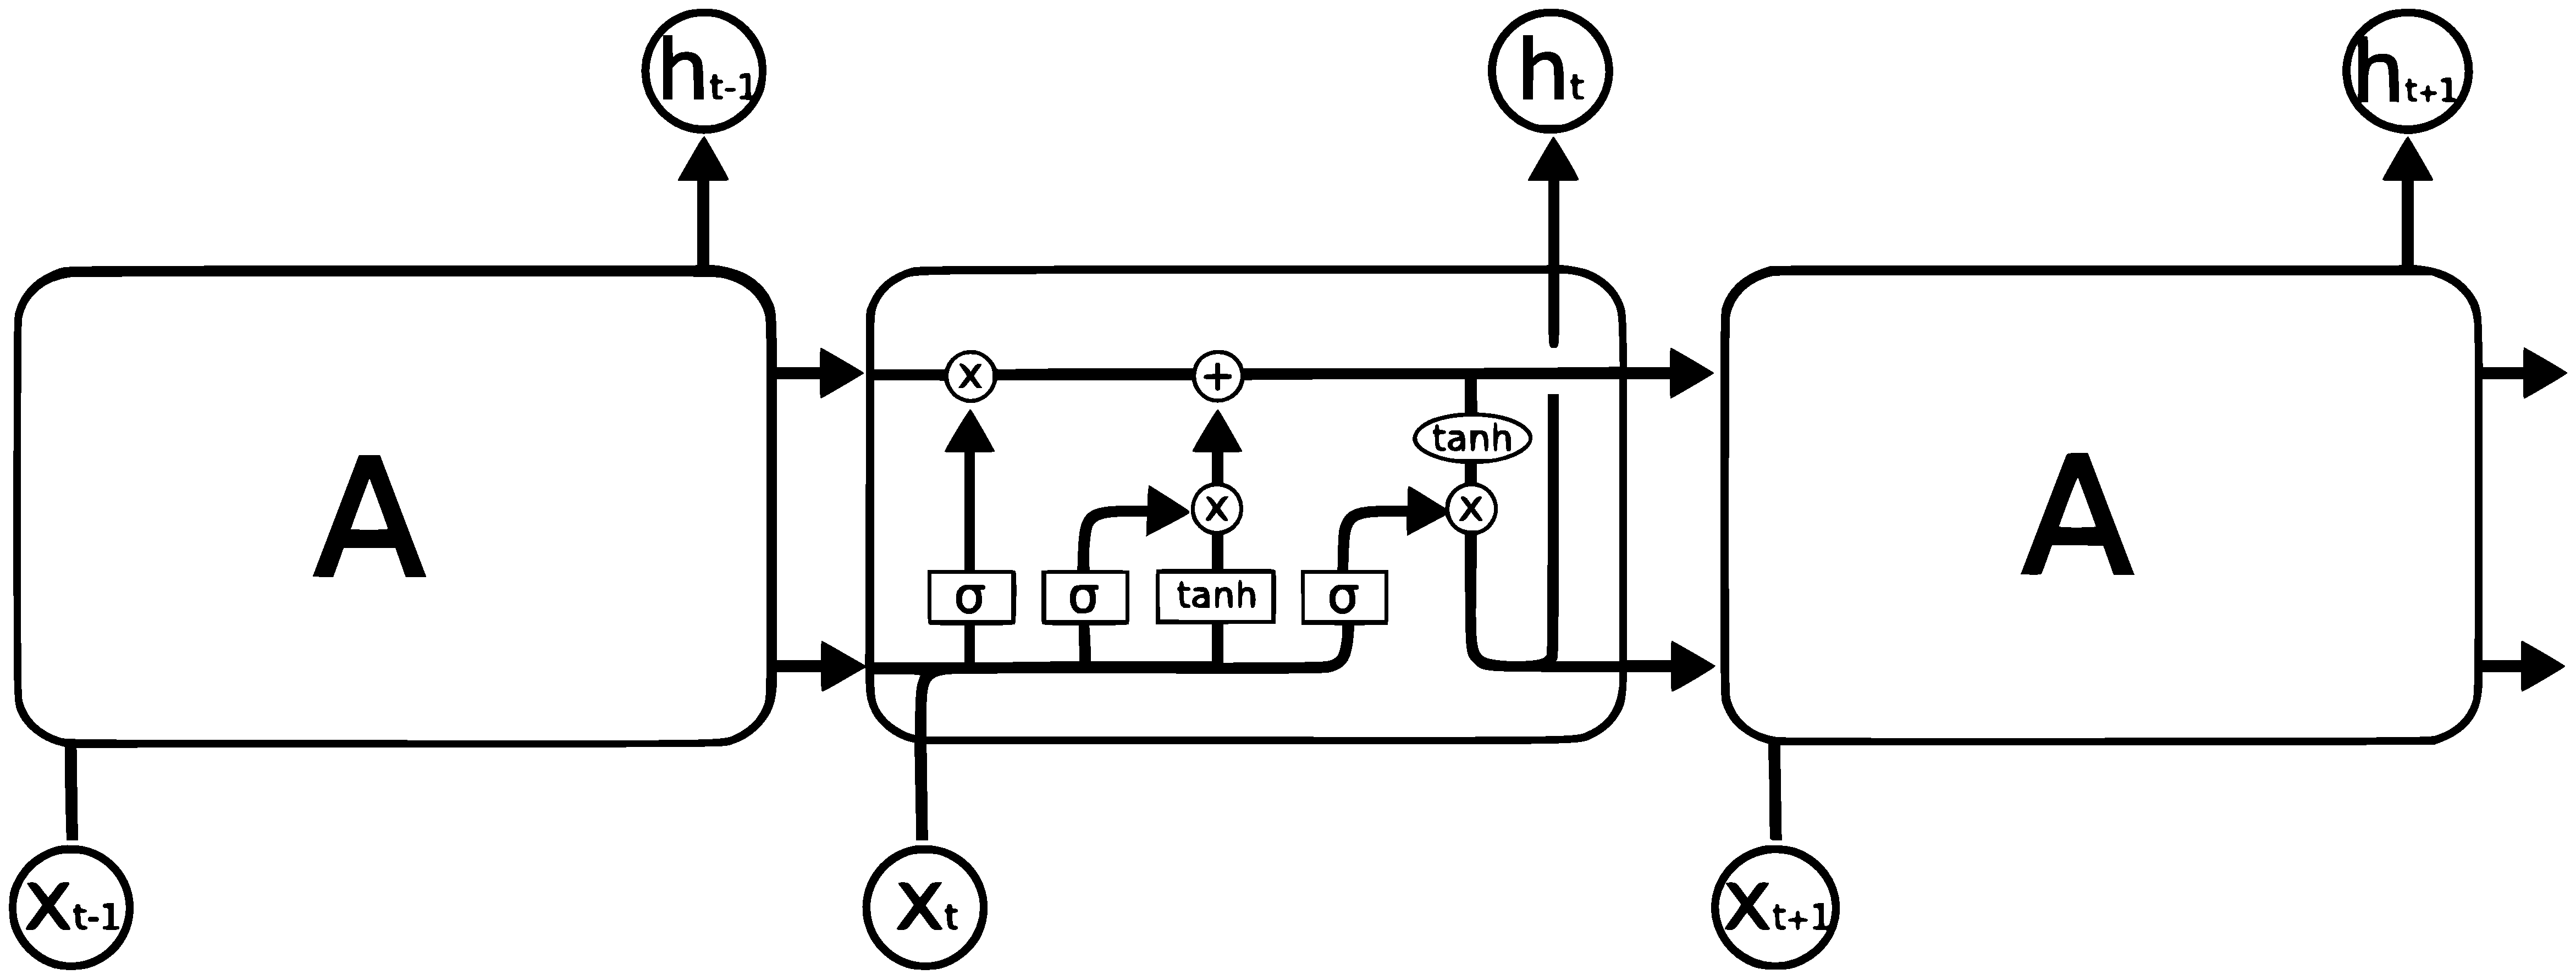
\includegraphics[width=\textwidth]	
	{machine_learning/01_Lstm_Diagram}
	\caption{LSTM Diagram.}
\end{figure}

\begin{figure}[H]
	\centering
	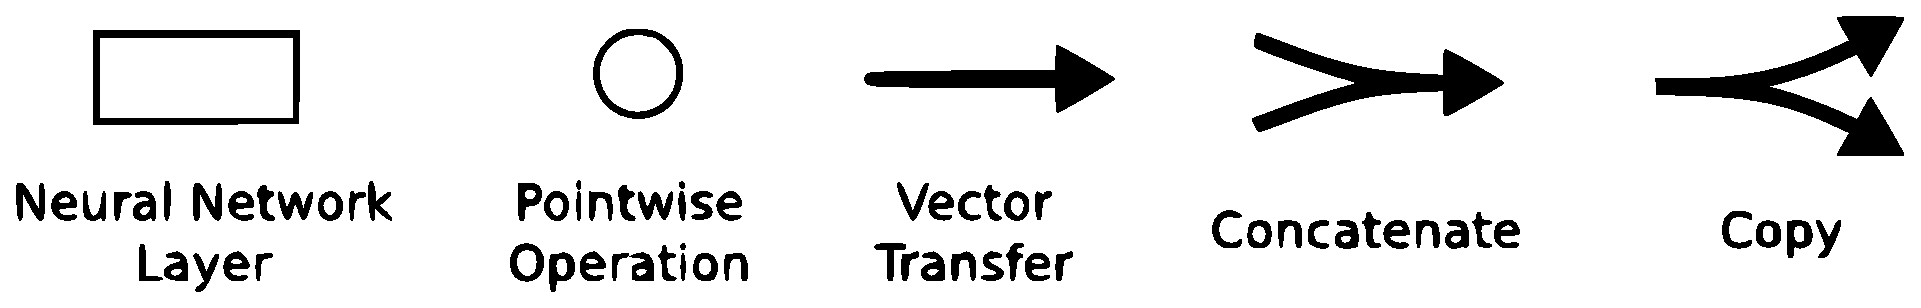
\includegraphics[width=\textwidth]		
	{machine_learning/02_Lstm_Notation}
	\caption{Diagram legend.}
\end{figure}

From the legend above, the lines represent vectors that pass
from the output of the previous note to the input of the 
current one. The dot denotes point wise operations, 
and the rectangle represents trained network layers.


A side by side description of the each layer of a LSTM and it`s mathematical formulation can be seen below, where the dot represents matrix multiplication.
The first layer represents the forget gate. This is where we decide which information to keep and which to discard. The layer outputs a value between zero and one for each input because of the sigmoid function(represented as sigma in the equations below), meaning that a value of zero represents data that will be complicity erased and so forth, while an absolute value of one represents data that will be left unchanged for the next iteration.    

\begin{figure}[H]
	\centering
	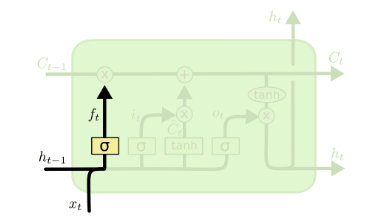
\includegraphics[width=0.5\textwidth]		
	{machine_learning/03_RForget}
	\begin{equation}
		 f= \sigma*(X.W_f+b_f) 
	\end{equation}	
	\caption{Forget Gate for concatenated inputs.}
	\label{fig:Forget}
\end{figure}

Similar to the forget gate, the LSTM structure also uses an update gate, to add new information to the system.
As seen in Figure \ref{fig:Update}, the update gate generates the new values that will be used. This takes place by multiplying the update gate to the input layer, represented by X` where a  hyperbolic tangent is used as the activation function. This is given as an example, as the Rectified Linear Unit(ReLU) or the softmax activation work perfectly fine as well.  
From the above mentioned gates a new internal state C can be computed as:
\begin{equation}
C_t= f * C_{t-1} + u*X` 
\end{equation}
Where the current state ($C_t$) is determined by what we want to forget ($f$), multiplied by the previous state ($C_t-1$) and added together with the update gate ($r$) times the input layer ($X`$).

\begin{figure}[H]
	\centering
		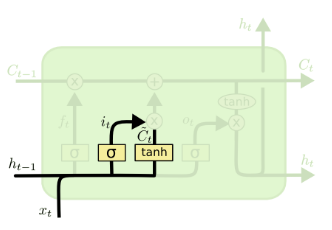
\includegraphics[width=0.5\textwidth]		
		{machine_learning/04_Update}
		\begin{equation}
		 	f= \sigma*(X.W_u+b_u) 
		\end{equation}	
		\begin{equation}	 
			 X`=tanh*(X.W_c+b_c)
	 	\end{equation}
	\caption{Update gate with the current state description.}
	\label{fig:Update}
\end{figure}

\begin{figure}[H]
	\centering
	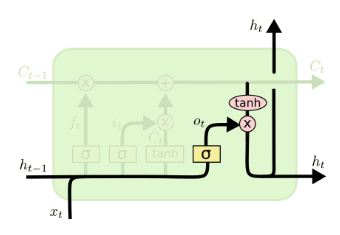
\includegraphics[width=0.5\textwidth]		
	{machine_learning/05_Result}
	\begin{equation}
		 r= \sigma*(X.W_r+b_r) 
	\end{equation}	
	\caption{Result gate added to the output function.}
	\label{fig:Result}
\end{figure}

The third and last gate is the result gate ($r$), which uses the previous internal state of the LSTM to generate a new internal state.
As such, the output of the neural network can be written as:

\begin{equation}
Y_t=softmax(H_t.W+b)
\end{equation}
%---------------------------------------------------
\subsection{Dropout}
Dropout is a regularization technique that involves shooting the neurons.
It is applied after the activation function of each layer with the notable exception of the input and output layer.
A percentage is used to determine the number of neurons that will remain in the networks.
For example, a .75 value in the dropout function means that only 75 percent of the neurons will remain active during the training phase.
At the test time all the neurons have to be present, meaning that a value of 1 has to be given to the dropout function to ensure a high accuracy rating.
This helps the network understand the information it is given as it cannot presume that other neurons in the same layer have been activated and it prevents the network from just memorizing the values that were given as inputs.
The snipped below shows how dropout is used in TensorFlow for a layer of a neural network, where pkeep is the percentage of the neurons that will remain active and the call for the dropout is made after the activation function, in this case the ReLU.

\begin{lstlisting}
pkeep = tf.palceholder(tf.float32)
YF = tf.nn.relu(tf.matmul(X, W)+ b)
Y = tf.nn.dropout(Yf, pkeep)
\end{lstlisting} 

\begin{figure}[H]
	\centering
	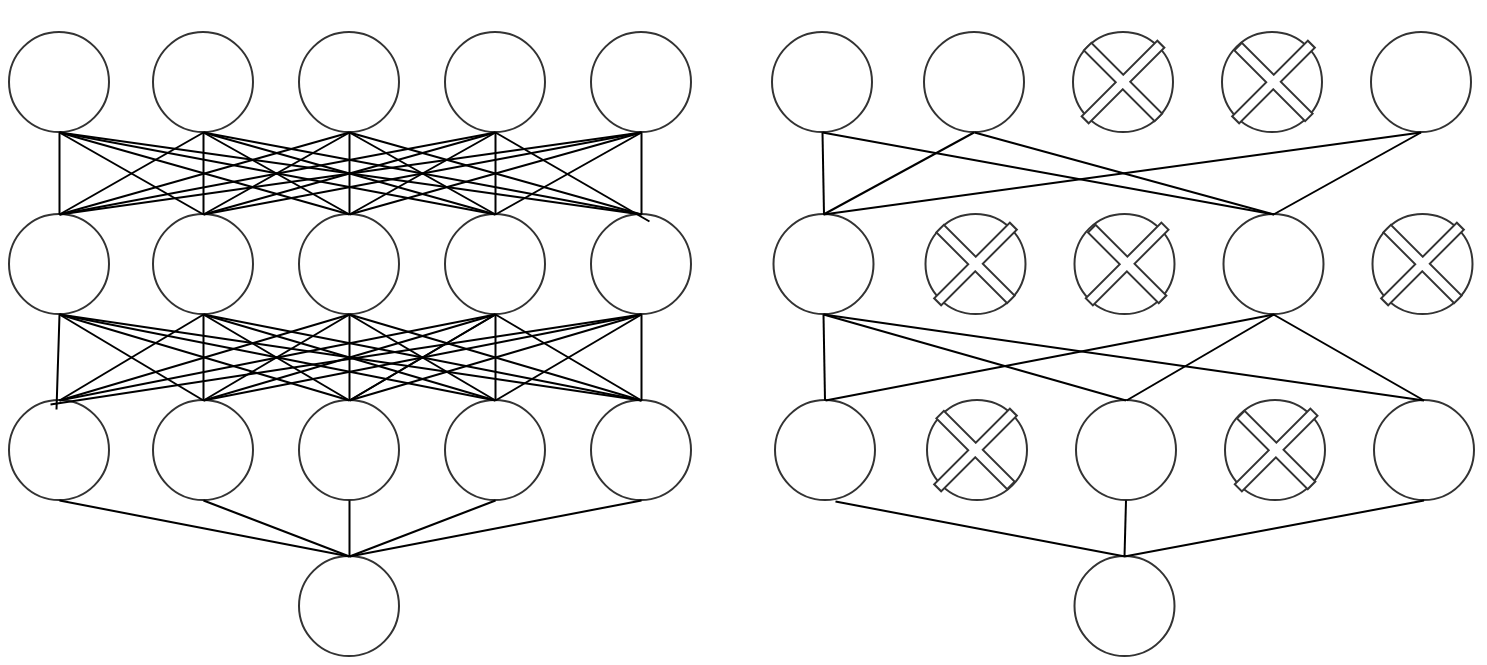
\includegraphics[width=\textwidth]		
	{machine_learning/06_Dropout}
	\caption{Dropout used on a generic network.}
\end{figure}

%---------------------------------------------------
\subsection{Batch normalisation}

Statistics can be computed for each batch that is fed to the neural network so the average and the standard deviation can be computed. After computing them, subtracting the average and dividing by the standard deviation rescales and recentre the output. 
In the equation, epsilon is added to avoid numerical problems as dividing by zero.

\begin{equation}
	X= \dfrac{x - avg(x)}{stdev(x) + \epsilon} 
\end{equation}

The recentre and rescaling of the values can cause problems to
the network for cases where data needs to be squeezed over 
to one side of the spectrum.
To solve those cases, two degrees of freedom are added, 
$\alpha$ and $\beta$, for each neuron. 
By assigning the $\alpha$ value to the $stdev(x)$ and the
$\beta$ to $-avg(x)$ there will always be a case where the batch
normalised value of x can be reverted to the original value.

\begin{equation}
	BN(x) = \alpha * X + \beta
\end{equation}

Batch normalisation(BN) is added before the activation function
because it takes use of the current weights and biases to
compute the average and standard deviation. 
The average and standard deviation is always computed on the
current weights and biases so the batch normalisation layer is
called between the weighted sum performed by the neurons and the
activation function. Because of the new values added by BN,
biases are no longer useful.
The $\beta$ value can take the value of the bias if no better
value was found.
In contrast to the ReLU, when using a sigmoid,
the scale parameter has to be used to make sure that
the data fits in the useful part of the activation function.
A representation of how to choose the right coefficients is
given in Table \ref{tab:Parameters}.

\begin{table}[htbp]
\centering
	\caption{Parameters for different activation functions.}
	\begin{tabular}{l c c}
	\toprule
  		& ReLU & Sigmoid \\\midrule
		Without BN &b & b  \\
		With BN & $\beta$ & $\alpha$, $\beta$  \\
	\bottomrule
	\end{tabular}
\label{tab:Parameters}
\end{table}

%---------------------------------------------------
\section{TensorFlow}

%---------------------------------------------------
TensorFlow provides multiple Application Programming Interfaces
(APIs) for machine learning. 
The lowest level API "TensorFlow Core" provides complete programming control \cite{tensorflow2015-whitepaper}. 
For those who require fine levels of control over their models,
TensorFlow Core is a well-suited tool for the job. There are higher level APIs that are built on top of TensorFlow Core.
These higher level APIs are typically easier to learn and use than Tensorflow Core \cite{tensorflow2015-whitepaper}.
In addition, the higher level APIs such as "tf.estimator" helps with managing data sets, estimators,
training and inferences (testing your trained network),
as well as, making repetitive tasks easier and more consistent
\cite{tensorflow2015-whitepaper}.\\

The subsection below will start with TensorFlow Core. 
In order to gain an understanding of the basic principles that TensorFlow has to offer, a model shall be made. 
In the subsection after that, the same model will be implemented with tf.estimator. 
Knowing TensorFlow Core principles will give us a great mental model of how things are working internally when we use the more compact higher level API.

\subsection{Tensors}
The central unit of data in TensorFlow is the tensor. 
A tensor consists of a set of primitive values shaped into an array of any number of dimensions. 
A tensor's rank is its number of dimensions. 
Here are some examples of tensors:

\begin{adjustbox}{width=\textwidth}
\begin{lstlisting}
3 # a rank 0 tensor; this is a scalar with shape []
[1., 2., 3.] # a rank 1 tensor; this is a vector with shape [3]
[[1., 2., 3.], [4., 5., 6.]] # a rank 2 tensor; a matrix with shape [2, 3]
[[[1., 2., 3.]], [[7., 8., 9.]]] # a rank 3 tensor with shape [2, 1, 3]
\end{lstlisting} 
\end{adjustbox}

\todo{I dont think the color option works well with the lstlisting}

\subsection{TensorFlow Core}
Getting Started With TensorFlow is done by using the import statement. 
This gives Python access to all of TensorFlow's classes,
methods, and symbols and is called by the following statement:

\begin{lstlisting}
import tensorflow as tf
\end{lstlisting}

All the programs written with the help of TensorFlow core are built around computational graphs. 
They are a series of operations arranged into a graph and connected by nodes. 
To see the outcome of a such a program, 
firstly the computational graph needs to be created and after that it needs to be run. 
This provides a contrast to normal code written in python and to display this, 
the print function for a tensorflow constant is called bellow.

\begin{lstlisting}
node1 = tf.constant(3.0, dtype=tf.float32)
node2 = tf.constant(4.0) # also tf.float32 implicitly
print(node1, node2)

Output:
Tensor("Const:0", shape=(), dtype=float32)
Tensor("Const_1:0", shape=(), dtype=float32) 
\end{lstlisting}

As seen above, printing an element does not show the value that it holds and it rather shows the technical details behind,
such as the element being a constant of type float32.
To investigate the contents of any element in tensorflow,
an object of type session needs to be defined.
When the new object is run, a new session is generated and the content of the element can be seen.
All code written is tensorflow core follows this basic principle.

\begin{lstlisting}
sess = tf.Session()
print(sess.run([node1, node2]))

Output:
[3.0]
\end{lstlisting}

Other basic elements in tensorflow are
placeholders(tf.placeholder), they can be changed to accept 
external inputs and variables. Variables allow the system to
change its outputs while keeping the seame inputs,
this allows the model to be trainable. 

\subsection{tf.train API}
The tf.train API holds optimizers that change each variable to minimize the loss function.
One of the simplest optimizers used to train neural networks is gradient descent.
Each variable is modified by the magnitude of the derivative of loss with respect to that variable.
Using a computer to gain these gradients is far less prone to error than doing it by hand.
Each of the gradients will point towards the minimum of the loss function and when solving for the gradient a step needs to be determined as the rate of change.
It is important to  have a small step as to not jump over the valley where the function takes its minimum value,
but in the beginning to reduce time and processing power a bigger step could be used.
One solution to this problem is to use a variable step input that changes as the gradients are determined.
TensorFlow can automatically produce derivatives given only a description of the model using the function tf.gradients.
For simplicity, optimizers typically do this for us.
\begin{lstlisting}
optimizer = tf.train.GradientDescentOptimizer(0.01)
train = optimizer.minimize(loss)
sess.run(train)
\end{lstlisting}
The gradient descent optimizer takes an input, defined at 0.01 in the example above,
that represents the step input or the rate of change for the gradients.

\subsection{tf.estimator API}
%---------------------------------------------------
To simplify the procedure of machine learning,
tf.estimator can be used as a higher-level library within Tensorflow.
It helps the user with running training and evaluation loops, managing data sets and much more. 
Making the entire process of writing an algorithm and maintaining it be less tedious.
Although the estimator library has a set of predefined models to make things easier, a custom model can be created while keeping the high
level abstraction of the data set, training and feeding.
A linear regression algorithm built with tf.estimator is included below to show how the library works \cite{Estimator}:

\begin{adjustbox}{width=\textwidth}
\begin{lstlisting}
import numpy as np
import tensorflow as tf

# Declare list of features. We only have one numeric feature. There are many
# other types of columns that are more complicated and useful.
feature_columns = [tf.feature_column.numeric_column("x", shape=[1])]

# An estimator is the front end to invoke training (fitting) and evaluation
# (inference). There are many predefined types like linear regression,
# linear classification, and many neural network classifiers and regressors.

# The following code provides an estimator that does linear regression.
estimator = tf.estimator.LinearRegressor(feature_columns=feature_columns)

# TensorFlow provides many helper methods to read and set up data sets.
# Here we use two data sets: one for training and one for evaluation
# We have to tell the function how many batches
# of data (num_epochs) we want and how big each batch should be.
x_train = np.array([1., 2., 3., 4.])
y_train = np.array([0., -1., -2., -3.])
x_eval = np.array([2., 5., 8., 1.])
y_eval = np.array([-1.01, -4.1, -7, 0.])
input_fn = tf.estimator.inputs.numpy_input_fn(
    {"x": x_train}, y_train, batch_size=4, num_epochs=None, shuffle=True)
train_input_fn = tf.estimator.inputs.numpy_input_fn(
    {"x": x_train}, y_train, batch_size=4, num_epochs=1000, shuffle=False)
eval_input_fn = tf.estimator.inputs.numpy_input_fn(
    {"x": x_eval}, y_eval, batch_size=4, num_epochs=1000, shuffle=False)

# We can invoke 1000 training steps by invoking the  method and passing the
# training data set.
estimator.train(input_fn=input_fn, steps=1000)

# Here we evaluate how well our model did.
train_metrics = estimator.evaluate(input_fn=train_input_fn)
eval_metrics = estimator.evaluate(input_fn=eval_input_fn)
print("train metrics: %r"% train_metrics)
print("eval metrics: %r"% eval_metrics)
\end{lstlisting}
\end{adjustbox}
%---------------------------------------------------

\section{Batch Size, Dropout and Learning Rate Comparison}
In order to gain a better understanding on how the different parameter values(batch size, dropout and learning rate) may effect the performance(training duration and test accuracy) of a neural network model, a small experiment was conducted.

This experiment consists of six test trials. For each test trail different parameter values were chosen, as shown in the table below.
%-------------------------------------------------------
%Table of Tests
\begin{table}[H]
\centering
	\caption{Six tests with different Parameter values.}
	\begin{tabular}{| l | c | c | c | c | c | c | c |} 
	\hline
		Parameters & 
		Test1 -\tikzcircle[orange, fill=orange]{3pt}- &
		Test2 -\tikzcircle[blue, fill=blue]{3pt}- &
		Test3 -\tikzcircle[red, fill=red]{3pt}- &
		Test4 -\tikzcircle[lightblue, fill=lightblue]{3pt}- &
		Test5 -\tikzcircle[pink, fill=pink]{3pt}- &
		Test6 -\tikzcircle[turquoise, fill=turquoise]{3pt}- \\ 
	\hline
		Batch Size & 
		2 \hfill 2 \hfill 2 & 
		20 \hfill 20 \hfill 20 & 
		20 \hfill 20 \hfill 20 &
		20 \hfill 20 \hfill 20 &
		50 \hfill 20 \hfill 20 &
		50 \hfill 20 \hfill 20 \\
	\hline
		Dropout & 
		0.05 & 0.05 & 0.00 & 0.50 & 0.05 & 0.05 \\
	\hline
		Learning Rate & 
		0.001 & 0.001 & 0.001 & 0.001 & 0.001 & 0.010 \\ 
	\hline
	\end{tabular}
\end{table}

info: batch size: (train, evaluation, test)\\
%-------------------------------------------------------

The tests were ran on a Bi-Directional Recurrent Neural Network
model found on the silicon valley data science GitHub repository
. The software we’re using is a mix of borrowed and inspired code from existing open source projects. 

%\cite{rubashkin2017}

\todo{figure out citing}

\subsection{Batch Size Test}
%-----------------------------------------------------
%Batch Size Test
\begin{table}[H]
\centering
	\caption{Three tests with different batch size values.}
	\begin{tabular}{| l | c | c | c | c |} 
	\hline
		Parameters & 
		Test1 -\tikzcircle[orange, fill=orange]{3pt}- &
		Test2 -\tikzcircle[blue, fill=blue]{3pt}- &
		Test5 -\tikzcircle[pink, fill=pink]{3pt}- \\
	\hline
		Batch Size & 
		2 \hfill 2 \hfill 2 & 
		20 \hfill 20 \hfill 20 & 
		50 \hfill 20 \hfill 20 \\
	\hline
		Dropout & 
		0.05 & 0.05 & 0.05 \\
	\hline
		Learning Rate & 
		0.001 & 0.001 & 0.001 \\ 
	\hline
	\end{tabular}
\end{table}
	%-------------------------------------------------
	%test error rate
\begin{figure}[H]
	\centering
	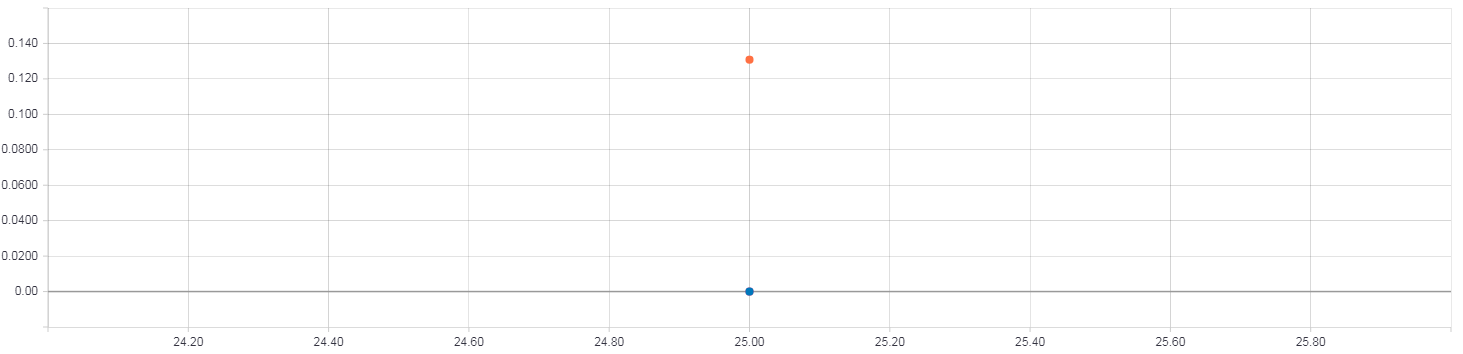
\includegraphics[width=\textwidth]		
	{machine_learning/graph_tests/batch_test/test_error_rate}
	\caption{Test error rate.}
\end{figure}
	%results
\begin{table}[H]
\centering
	\caption{Test error rate results.}
	\begin{tabular}{| l | c | c | c |}
	\hline
		Tests & Value & Epoch & Duration \\
	\hline
		Test1 -\tikzcircle[orange, fill=orange]{3pt}- &
		0.1308 & 25.00 & 0s\\
	\hline
		Test2 -\tikzcircle[blue, fill=blue]{3pt}- &
		0.000 & 25.00 & 0s\\
	\hline
		Test5 -\tikzcircle[pink, fill=pink]{3pt}- &
		0.000 & 25.00 & 0s\\
	\hline
	\end{tabular}
\end{table}
	%-------------------------------------------------
	%training error rate
\begin{figure}[H]
	\centering
	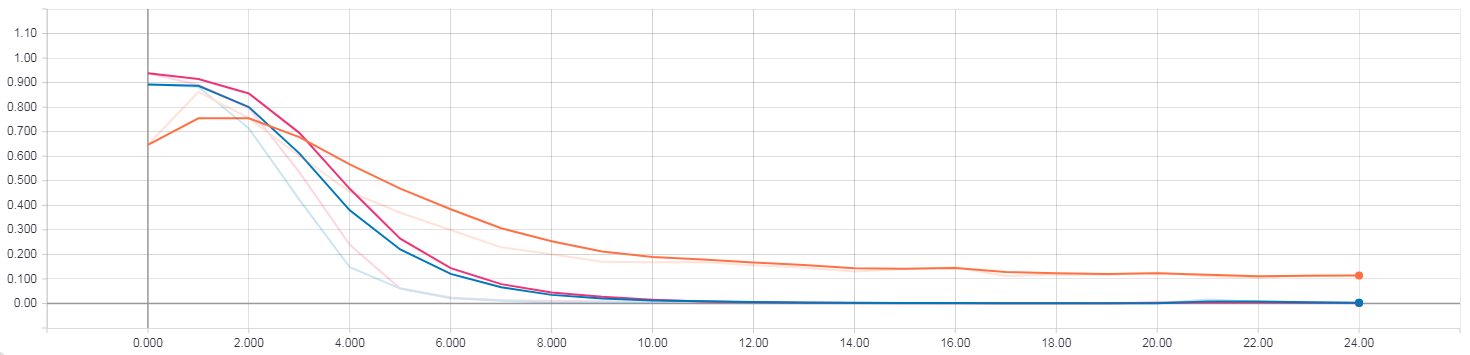
\includegraphics[width=\textwidth]		
	{machine_learning/graph_tests/batch_test/train_error_rate}
	\caption{Training error rate.}
\end{figure}
	%results
\begin{table}[H]
\centering
	\caption{Training error rate results.}
	\begin{tabular}{| l | c | c | c |}
	\hline
		Tests & Value & Epoch & Duration \\
	\hline
		Test1 -\tikzcircle[orange, fill=orange]{3pt}- &
		0.1148 & 24.00 & 1h 26m 13s\\
	\hline
		Test2 -\tikzcircle[blue, fill=blue]{3pt}- &
		9.5073e-4 & 24.00 & 18m 50s\\
	\hline
		Test5 -\tikzcircle[pink, fill=pink]{3pt}- &
		5.1858e-4 & 24.00 & 14m 50s\\
	\hline
	\end{tabular}
\end{table}	
	%-------------------------------------------------
%-----------------------------------------------------

\subsection{Dropout Test}
%-----------------------------------------------------
%Dropout Test
\begin{table}[H]
\centering
	\caption{Three tests with different dropout values.}
	\begin{tabular}{| l | c | c | c | c |} 
	\hline
		Parameters & 
		Test2 -\tikzcircle[blue, fill=blue]{3pt}- &
		Test3 -\tikzcircle[red, fill=red]{3pt}- &
		Test4 -\tikzcircle[lightblue, fill=lightblue]{3pt}- \\
	\hline
		Batch Size & 
		20 \hfill 20 \hfill 20 & 
		20 \hfill 20 \hfill 20 &
		20 \hfill 20 \hfill 20 \\
	\hline
		Dropout & 
		0.05 & 0.00 & 0.50 \\
	\hline
		Learning Rate & 
		0.001 & 0.001 & 0.001 \\ 
	\hline
	\end{tabular}
\end{table}
	%-------------------------------------------------
	%test error rate
\begin{figure}[H]
	\centering
	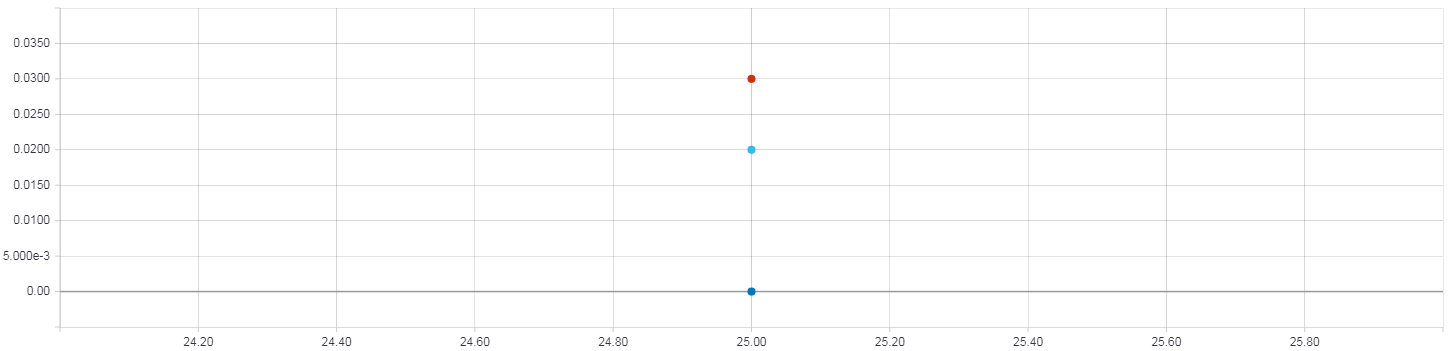
\includegraphics[width=\textwidth]		
	{machine_learning/graph_tests/dropout_test/test_error_rate}
	\caption{Test error rate.}
\end{figure}
	%results
\begin{table}[H]
\centering
	\caption{Test error rate results.}
	\begin{tabular}{| l | c | c | c |}
	\hline
		Tests & Value & Epoch & Duration \\
	\hline
		Test2 -\tikzcircle[blue, fill=blue]{3pt}- &
		0.000 & 25.00 & 0s\\
	\hline
		Test3 -\tikzcircle[red, fill=red]{3pt}- &
		0.030 & 25.00 & 0s\\
	\hline
		Test4 -\tikzcircle[lightblue, fill=lightblue]{3pt}- &
		0.020 & 25.00 & 0s\\
	\hline
	\end{tabular}
\end{table}		
	%-------------------------------------------------
	%training error rate
\begin{figure}[H]
	\centering
	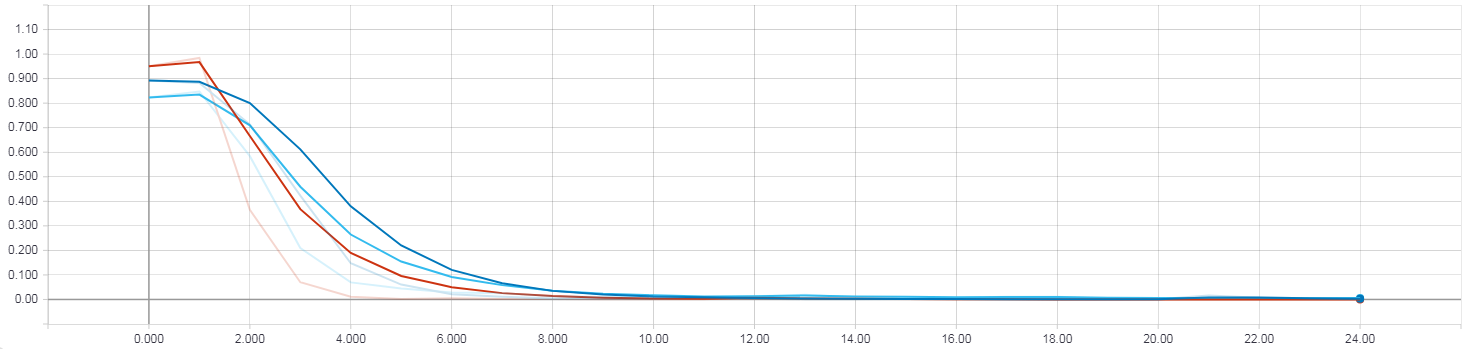
\includegraphics[width=\textwidth]		
	{machine_learning/graph_tests/dropout_test/train_error_rate}
	\caption{Training error rate.}
\end{figure}
	%results
\begin{table}[H]
\centering
	\caption{Training error rate results.}
	\begin{tabular}{| l | c | c | c |}
	\hline
		Tests & Value & Epoch & Duration \\
	\hline
		Test2 -\tikzcircle[blue, fill=blue]{3pt}- &
		9.5973e-4 & 24.00 & 18m 50s\\
	\hline
		Test3 -\tikzcircle[red, fill=red]{3pt}- &
		0.000 & 24.00 & 18m 5s\\
	\hline
		Test4 -\tikzcircle[lightblue, fill=lightblue]{3pt}- &
		6.3331e-3 & 24.00 & 18m 10s\\
	\hline
	\end{tabular}
\end{table}		
	%-------------------------------------------------
%-----------------------------------------------------

\subsection{Learning Rate Test}
%-----------------------------------------------------
%Learning Rate Test
\begin{table}[H]
\centering
	\caption{Two tests with different learning rate values.}
	\begin{tabular}{| l | c | c | c |} 
	\hline
		Parameters & 
		Test5 -\tikzcircle[pink, fill=pink]{3pt}- &
		Test6 -\tikzcircle[turquoise, fill=turquoise]{3pt}- \\ 
	\hline
		Batch Size & 
		50 \hfill 20 \hfill 20 &
		50 \hfill 20 \hfill 20 \\
	\hline
		Dropout & 0.05 & 0.05 \\
	\hline
		Learning Rate & 0.001 & 0.010 \\ 
	\hline
	\end{tabular}
\end{table}
	%-------------------------------------------------
	%test error rate
\begin{figure}[H]
	\centering
	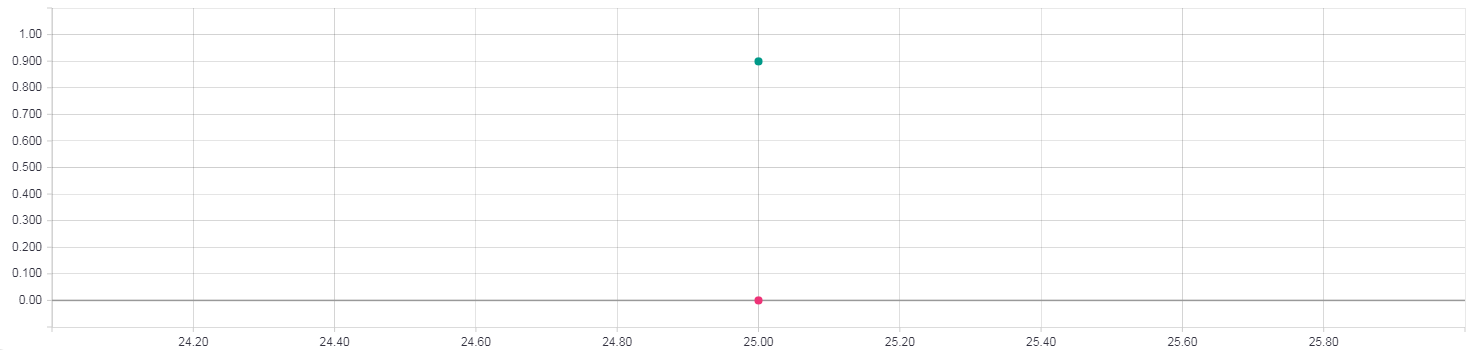
\includegraphics[width=\textwidth]		
	{machine_learning/graph_tests/learning_rate_test/test_error_rate}
	\caption{Test error rate.}
\end{figure}
	%results
\begin{table}[H]
\centering
	\caption{Test error rate results.}
	\begin{tabular}{| l | c | c | c |}
	\hline
		Tests & Value & Epoch & Duration \\
	\hline
		Test5 -\tikzcircle[pink, fill=pink]{3pt}- &
		0.000 & 25.00 & 0s\\
	\hline
		Test6 -\tikzcircle[turquoise, fill=turquoise]{3pt}- &
		0.8992 & 25.00 & 0s\\
	\hline
	\end{tabular}
\end{table}		
	%-------------------------------------------------
	%training error rate
\begin{figure}[H]
	\centering
	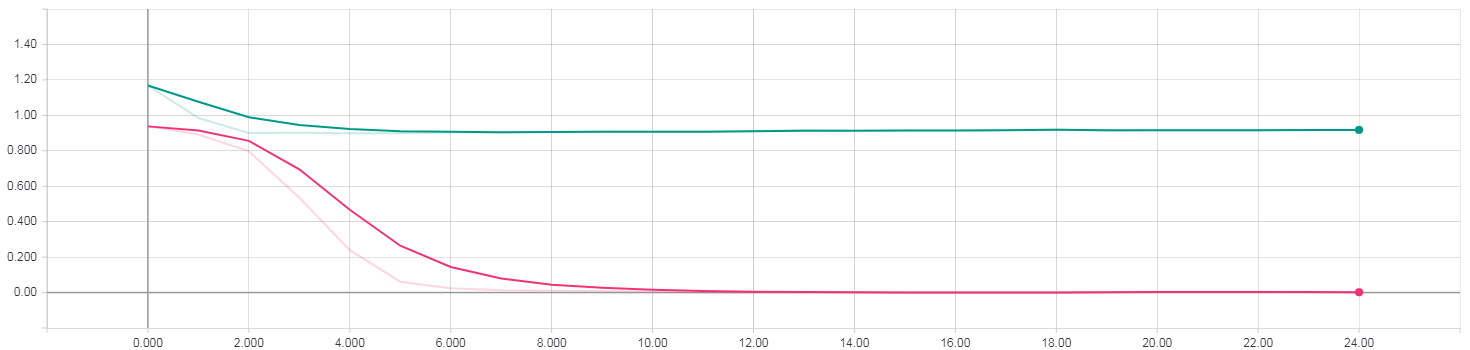
\includegraphics[width=\textwidth]		
	{machine_learning/graph_tests/learning_rate_test/train_error_rate}
	\caption{Training error rate.}
\end{figure}
	%results
\begin{table}[H]
\centering
	\caption{Training error rate results.}
	\begin{tabular}{| l | c | c | c |}
	\hline
		Tests & Value & Epoch & Duration \\
	\hline
		Test5 -\tikzcircle[pink, fill=pink]{3pt}- &
		5.1858e-4 & 24.00 & 14m 50s\\
	\hline
		Test6 -\tikzcircle[turquoise, fill=turquoise]{3pt}- &
		0.9188 & 24.00 & 12m 29s\\
	\hline
	\end{tabular}
\end{table}		
	%-------------------------------------------------
%---------------------------------------------------


	
	\chapter{Distributed speech recognizer}\label{ch:distributed_speech_recognizer}

\section{Virtual Private Network(VPN)}


\begin{figure}[h]
	\centering
	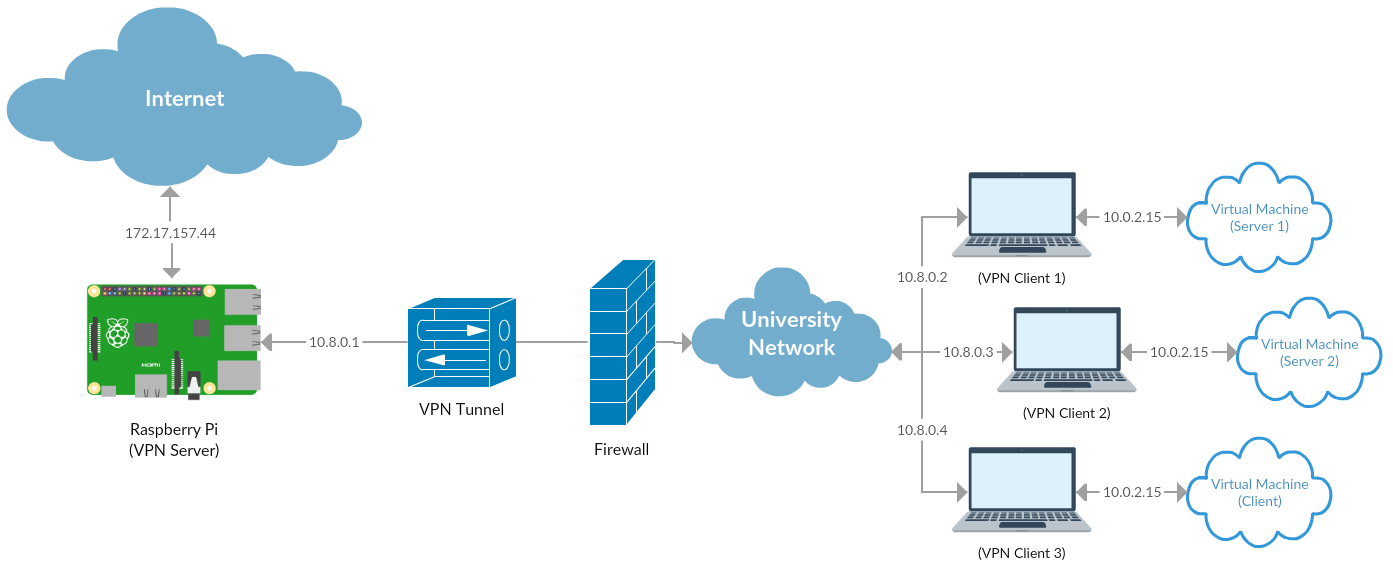
\includegraphics[width=\textwidth]		
	{distributed_speech_recognizer/00_Network_Infrastructure}
	\caption{Virtual private network to university.}
	\label{fig:DSR}
\end{figure}



\section{Sockets}
	
	\chapter{Knowledge-based IR system}\label{ch:knowledge_based_IR_system}

\section{The document retrieval system}

\section{The question answering system}
	
	\chapter{Model Development}\label{ch:model_development}
One of the goals for this project was to research, design and compare different neural network topologies. 
Some of these were feed-forward and recurrent.
Continuing, some neural networks were made deep, first by adding fully connected layers to the existing type feed-forward, CNN or RNN.
Different configurations were tested, some proving to be efficient for achieving designated goals, and some less so.
Subject to further research, we found that recurrent neural networks work best for speech recognition.
Therefore  the following comparison will be based on different RNNs configurations.\\\\

\section{Neural Network Comparison}\label{sec:NNComparison}

In this chapter two models are developed based on the simple LSTM model from the silicon-valley-data-science RNN tutorial \cite{rubashkin2017}. Firstly these models (including "their simple LSTM model") will be trained and tested on a small data set with the numbers:\\\\
$\left\{zero, one, two, three, four, five, six, seven, eight, nine \right\}$,\\\\
the same data used in Chapter \ref{ch:machine_learning} for the parameter comparison. After that, the best performing model shall be picked for a more detailed description (with code) and further training with a bigger data set of the English language.\\\\
Before the comparison of the 3 models, lets take a look at their structure in the following diagrams.
As mentioned earlier the two models that were developed are based on the silicon-valley-data-science simple LSTM model. Their model consist of two LSTM layers as shown in the diagram below (Figure \ref{fig:simple_LSTM}).
\begin{figure}[H]
	\centering
	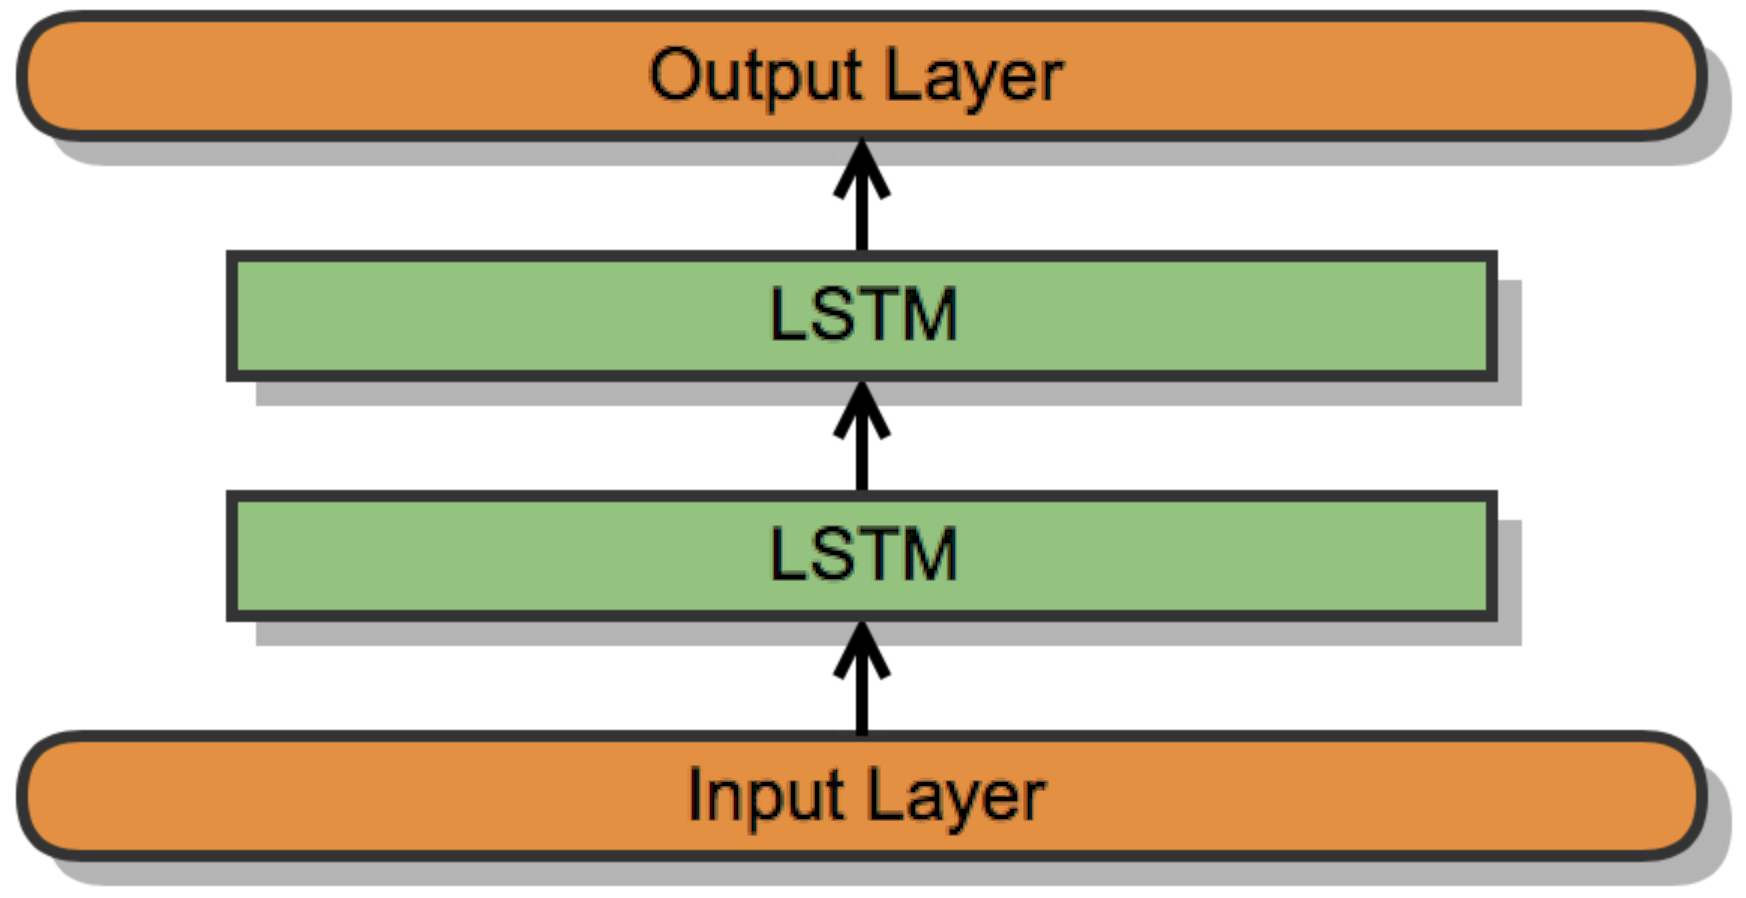
\includegraphics[width=.35\textwidth]		
	{model_development/01_simpleLSTM}
	\caption{Simple LSTM model.}
	\label{fig:simple_LSTM}
\end{figure}
Based on model above, it was decided among us to make an addition of two fully connected (FC) layers before and one FC layer after the two LSTM layers (shown in Figure \ref{fig:simple_LSTMFC}), with the desire of gaining better accuracy.
\begin{figure}[H]
	\centering
	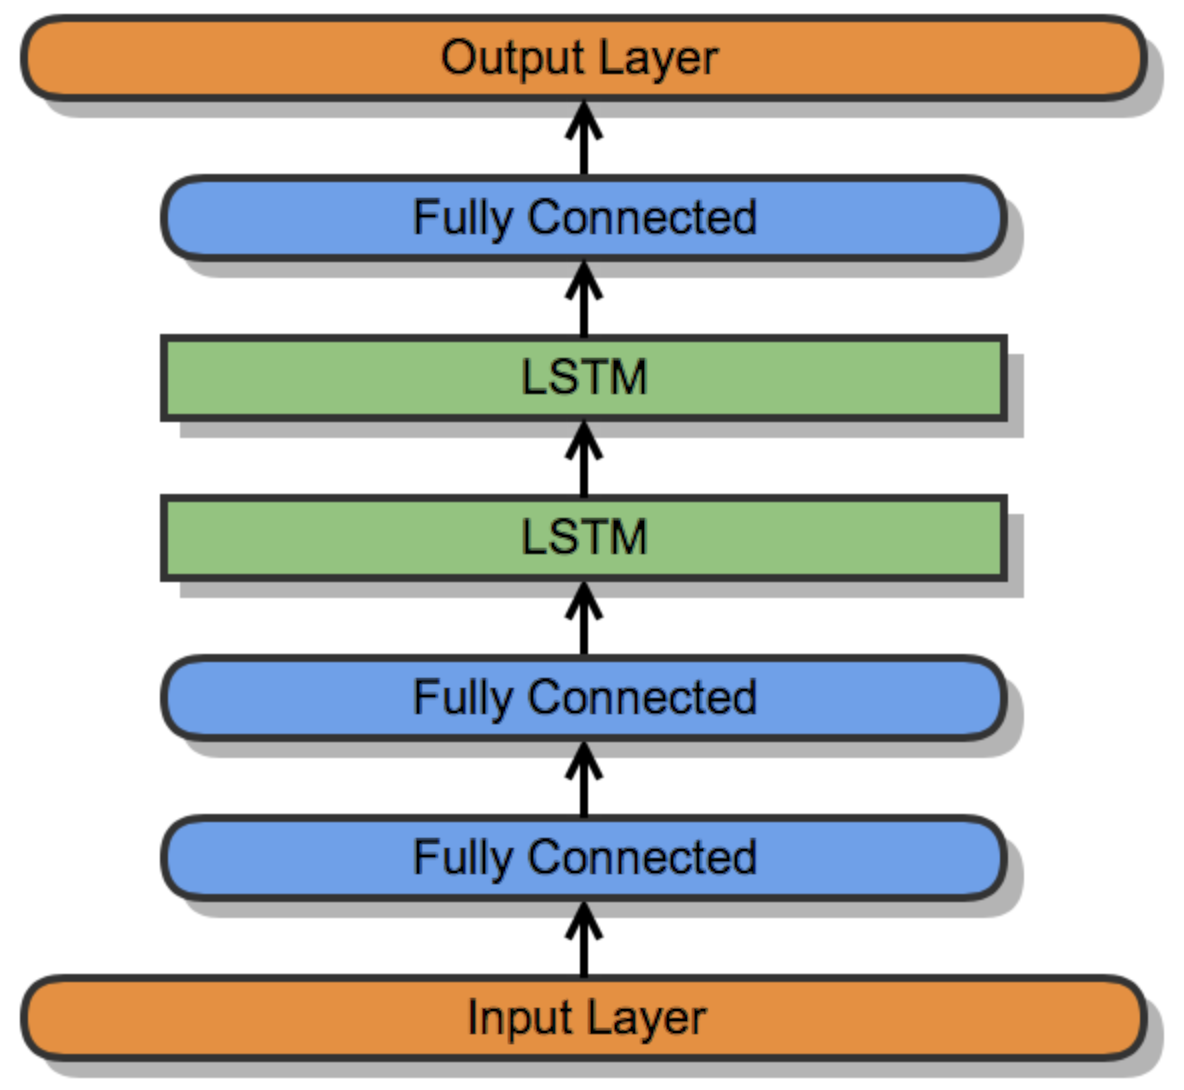
\includegraphics[width=.35\textwidth]		
	{model_development/02_simpleLSTMFC}
	\caption{Simple LSTM model with fully connected layers.}
	\label{fig:simple_LSTMFC}
\end{figure}
After that, a decision was made to replace the to LSTM layers in the model above with one Bi-Directional LSTM layers (seen in Figure \ref{fig:BiRNNFC}), again with the desire to make a more accurate model
\begin{figure}[H]
	\centering
	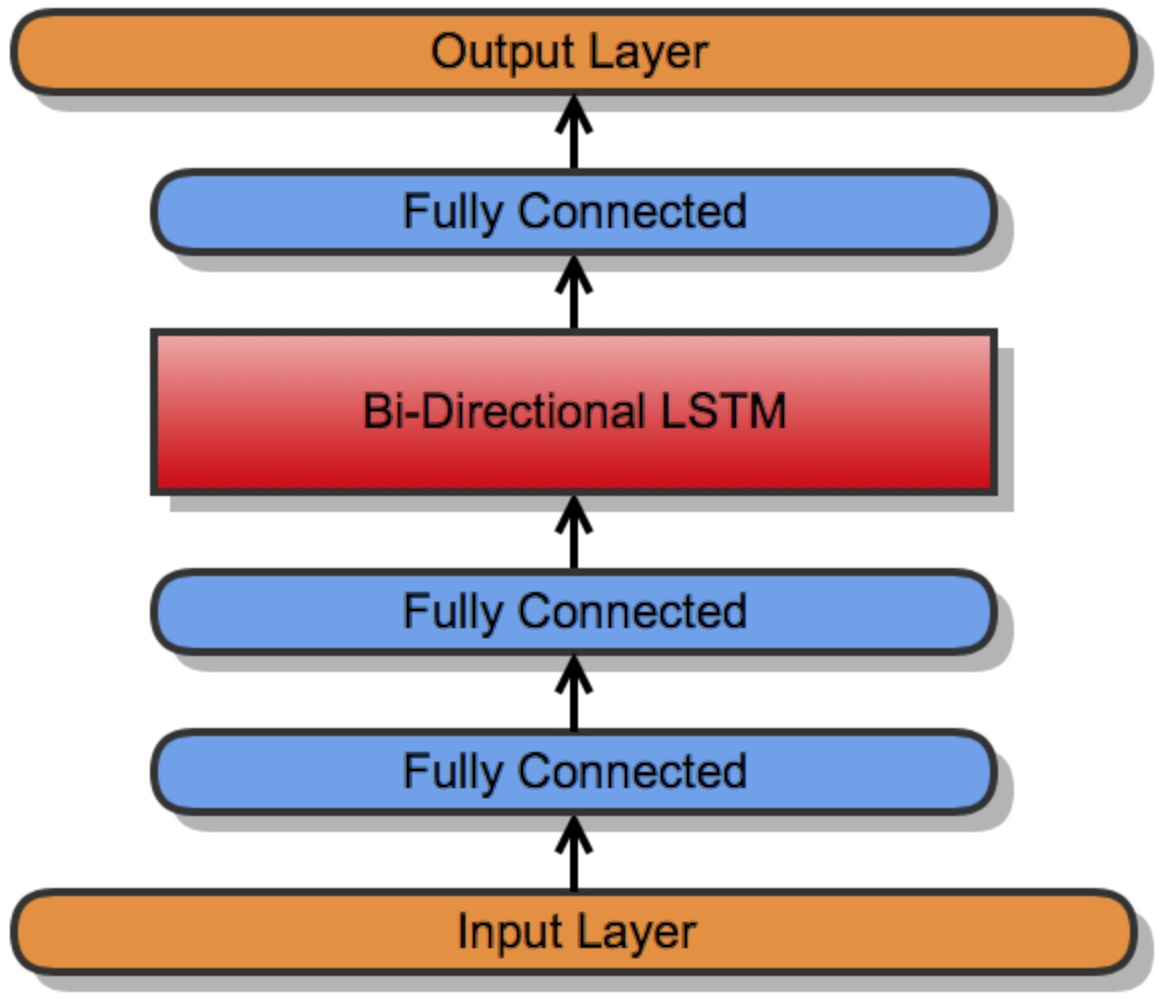
\includegraphics[width=.35\textwidth]		
	{model_development/03_BiRNN}
	\caption{BiRNN model with fully connected layers.}
	\label{fig:BiRNNFC}
\end{figure}

In order to have a fair comparison between these model the parameters values were made to be the same for all models as shown in Table \ref{tab:3models_tab}.
The respective models are mapped to the described ones in Table \ref{tab:3_models}. For the interested reader an expanded version in appendix \ref{ch:appClabel}.
\begin{table}[H]
\centering
    \caption{Parameter values of the three model.}
    \begin{tabular}{| l | c | c | c | c |} 
    \hline
        Parameters & 
        Model1 -\tikzcircle[pink, fill=pink]{3pt}- &
        Model2 -\tikzcircle[red, fill=red]{3pt}- &
        Model3 -\tikzcircle[turquoise, fill=turquoise]{3pt}-\\
    \hline
        Batch Size & 
        50 \hfill 20 \hfill 20 & 
        50 \hfill 20 \hfill 20 & 
        50 \hfill 20 \hfill 20 \\
    \hline
        Dropout & 
        0.05 & 0.05 & 0.05 \\
    \hline
        Learning Rate & 
        0.001 & 0.001 & 0.001 \\ 
    \hline
    \end{tabular}
    \label{tab:3models_tab}
\end{table}
\begin{table}[H]
\centering
	\caption{Models.}
	\begin{tabular}{ l  c }
	Model1 -\tikzcircle[pink, fill=pink]{3pt}- &
	(simple LSTM Model)\\
	Model2 -\tikzcircle[red, fill=red]{3pt}- &
	(simple LSTM + FC Model)\\
	Model3 -\tikzcircle[turquoise, fill=turquoise]{3pt}- &
	(BiRNN + FC Model)\\
	\end{tabular}
	\label{tab:3_models}
\end{table}

The following graph (Fig. \ref{fig:test_error_fig}) and
table (Tab. \ref{tab:test_error_tab}) represent the error
rate for the test data set. The results show that Model1 has $\sim 20\%$ word error rate (WER) while
Model2 and Model3 is $\sim 8\%$ and $\sim 0\%$ WER respectively.

\begin{figure}[H]
	\centering
	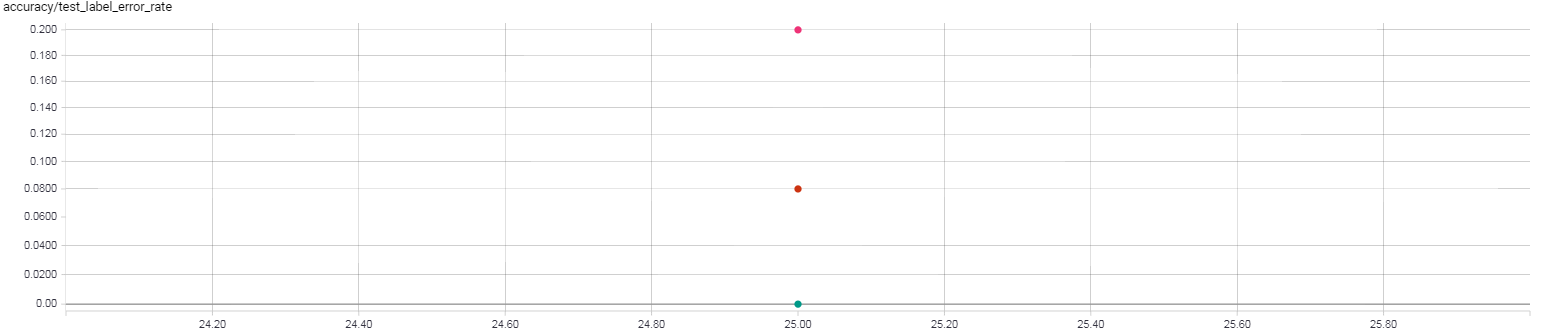
\includegraphics[width=\textwidth]		
	{model_development/3models_comparison/test_error_rate_3models}
	\caption{Test error rate.}
	\label{fig:test_error_fig}
\end{figure}

\begin{table}[H]
\centering
	\caption{Test error rate results.}
	\begin{tabular}{| l | c | c | c |}
	\hline
	Models & Value & Epoch & Duration \\
	\hline
	Model1 -\tikzcircle[pink, fill=pink]{3pt}- &
	0.200 & 25.00 & 0s\\
	\hline
	Model2 -\tikzcircle[red, fill=red]{3pt}- &
	0.080 & 25.00 & 0s\\
	\hline
	Model3 -\tikzcircle[turquoise, fill=turquoise]{3pt}- &
	0.000 & 25.00 & 0s\\
	\hline
	\end{tabular}
	\label{tab:test_error_tab}
\end{table}

The following graph (Fig. \ref{fig:validation_error_fig}) and
table (Tab. \ref{tab:validation_error_tab}) represent the error
rate for the validation data set. The results show that Model1 has took $\sim 7m 9s$ to complete training while
Model2 and Model3 is $\sim 9m 8s$ and $\sim 11m 49s$ respectively.

\begin{figure}[H]
	\centering
	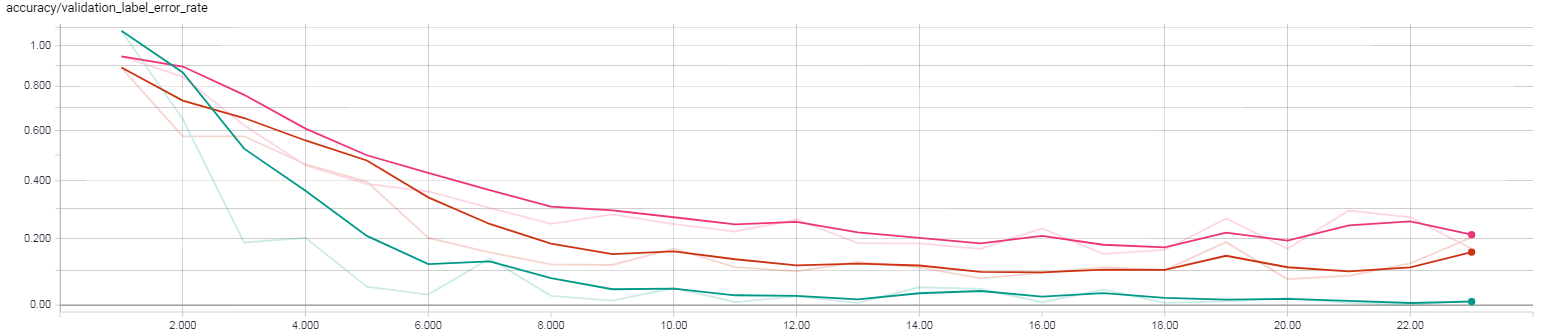
\includegraphics[width=\textwidth]		
	{model_development/3models_comparison/validation_error_rate_3models}
	\caption{Validation error rate.}
	\label{fig:validation_error_fig}
\end{figure}

\begin{table}[H]
\centering
	\caption{Validation error rate results.}
	\begin{tabular}{| l | c | c | c |}
	\hline
	Models & Value & Epoch & Duration \\
	\hline
	Model1 -\tikzcircle[pink, fill=pink]{3pt}- &
	0.1669 & 23.00 & 7m 9s\\
	\hline
	Model2 -\tikzcircle[red, fill=red]{3pt}- &
	0.2030 & 23.00 & 9m 8s\\
	\hline
	Model3 -\tikzcircle[turquoise, fill=turquoise]{3pt}- &
	0.01398 & 23.00 & 11m 49s\\
	\hline
	\end{tabular}
	\label{tab:validation_error_tab}
\end{table}

The final results show that Model1 was improved by adding the fully connected layers (Model2) from $\sim 20\%$ to $\sim 8\%$ WER and further improved by the replacing the two LSTMs by one Bi-Directional LSTM layer (Model3) from $\sim 8\%$ to $\sim 0\%$ WER.
The graph for the validation error rate (Figure \ref{fig:validation_error_fig}) clearly shows the three distinct lines in "parallel" with each other. The top line being the least accurate and the bottom one being the most.

\section{Model Description}
<<<<<<< HEAD
As shown in Chapter \ref{ch:model_development} under Neural Network Comparison, the model that is used in this DSR system is based on a bidirectional, Long-short Term Memory, recurrent neural network.
=======
As shown in Chapter \ref{ch:model_development} under Neural Network Comparison, the model that is used in this DSR system is based on a bidirectional, Long-short Term Memory , recurrent neural network.
>>>>>>> 65e88503a18a0da70a792d603725940342bca980
This recurrent network is using the standard TensorFlow implementation of an LSTM cell, called "BasicLSTMCell", and used as a bidirectional layer. 
There are two cells in the layer, one "forward" direction and one "backward" direction.
Each cell is unrolled 1024 times, giving the layer 2048 elements. 
The purpose is to recognize the context of the text, thus improving the prediction accuracy.
The complete topology for the network is as follows: \\\\
<<<<<<< HEAD
\todo{Make full page png}
=======

>>>>>>> 65e88503a18a0da70a792d603725940342bca980
\begin{figure}[H]
	\centering
	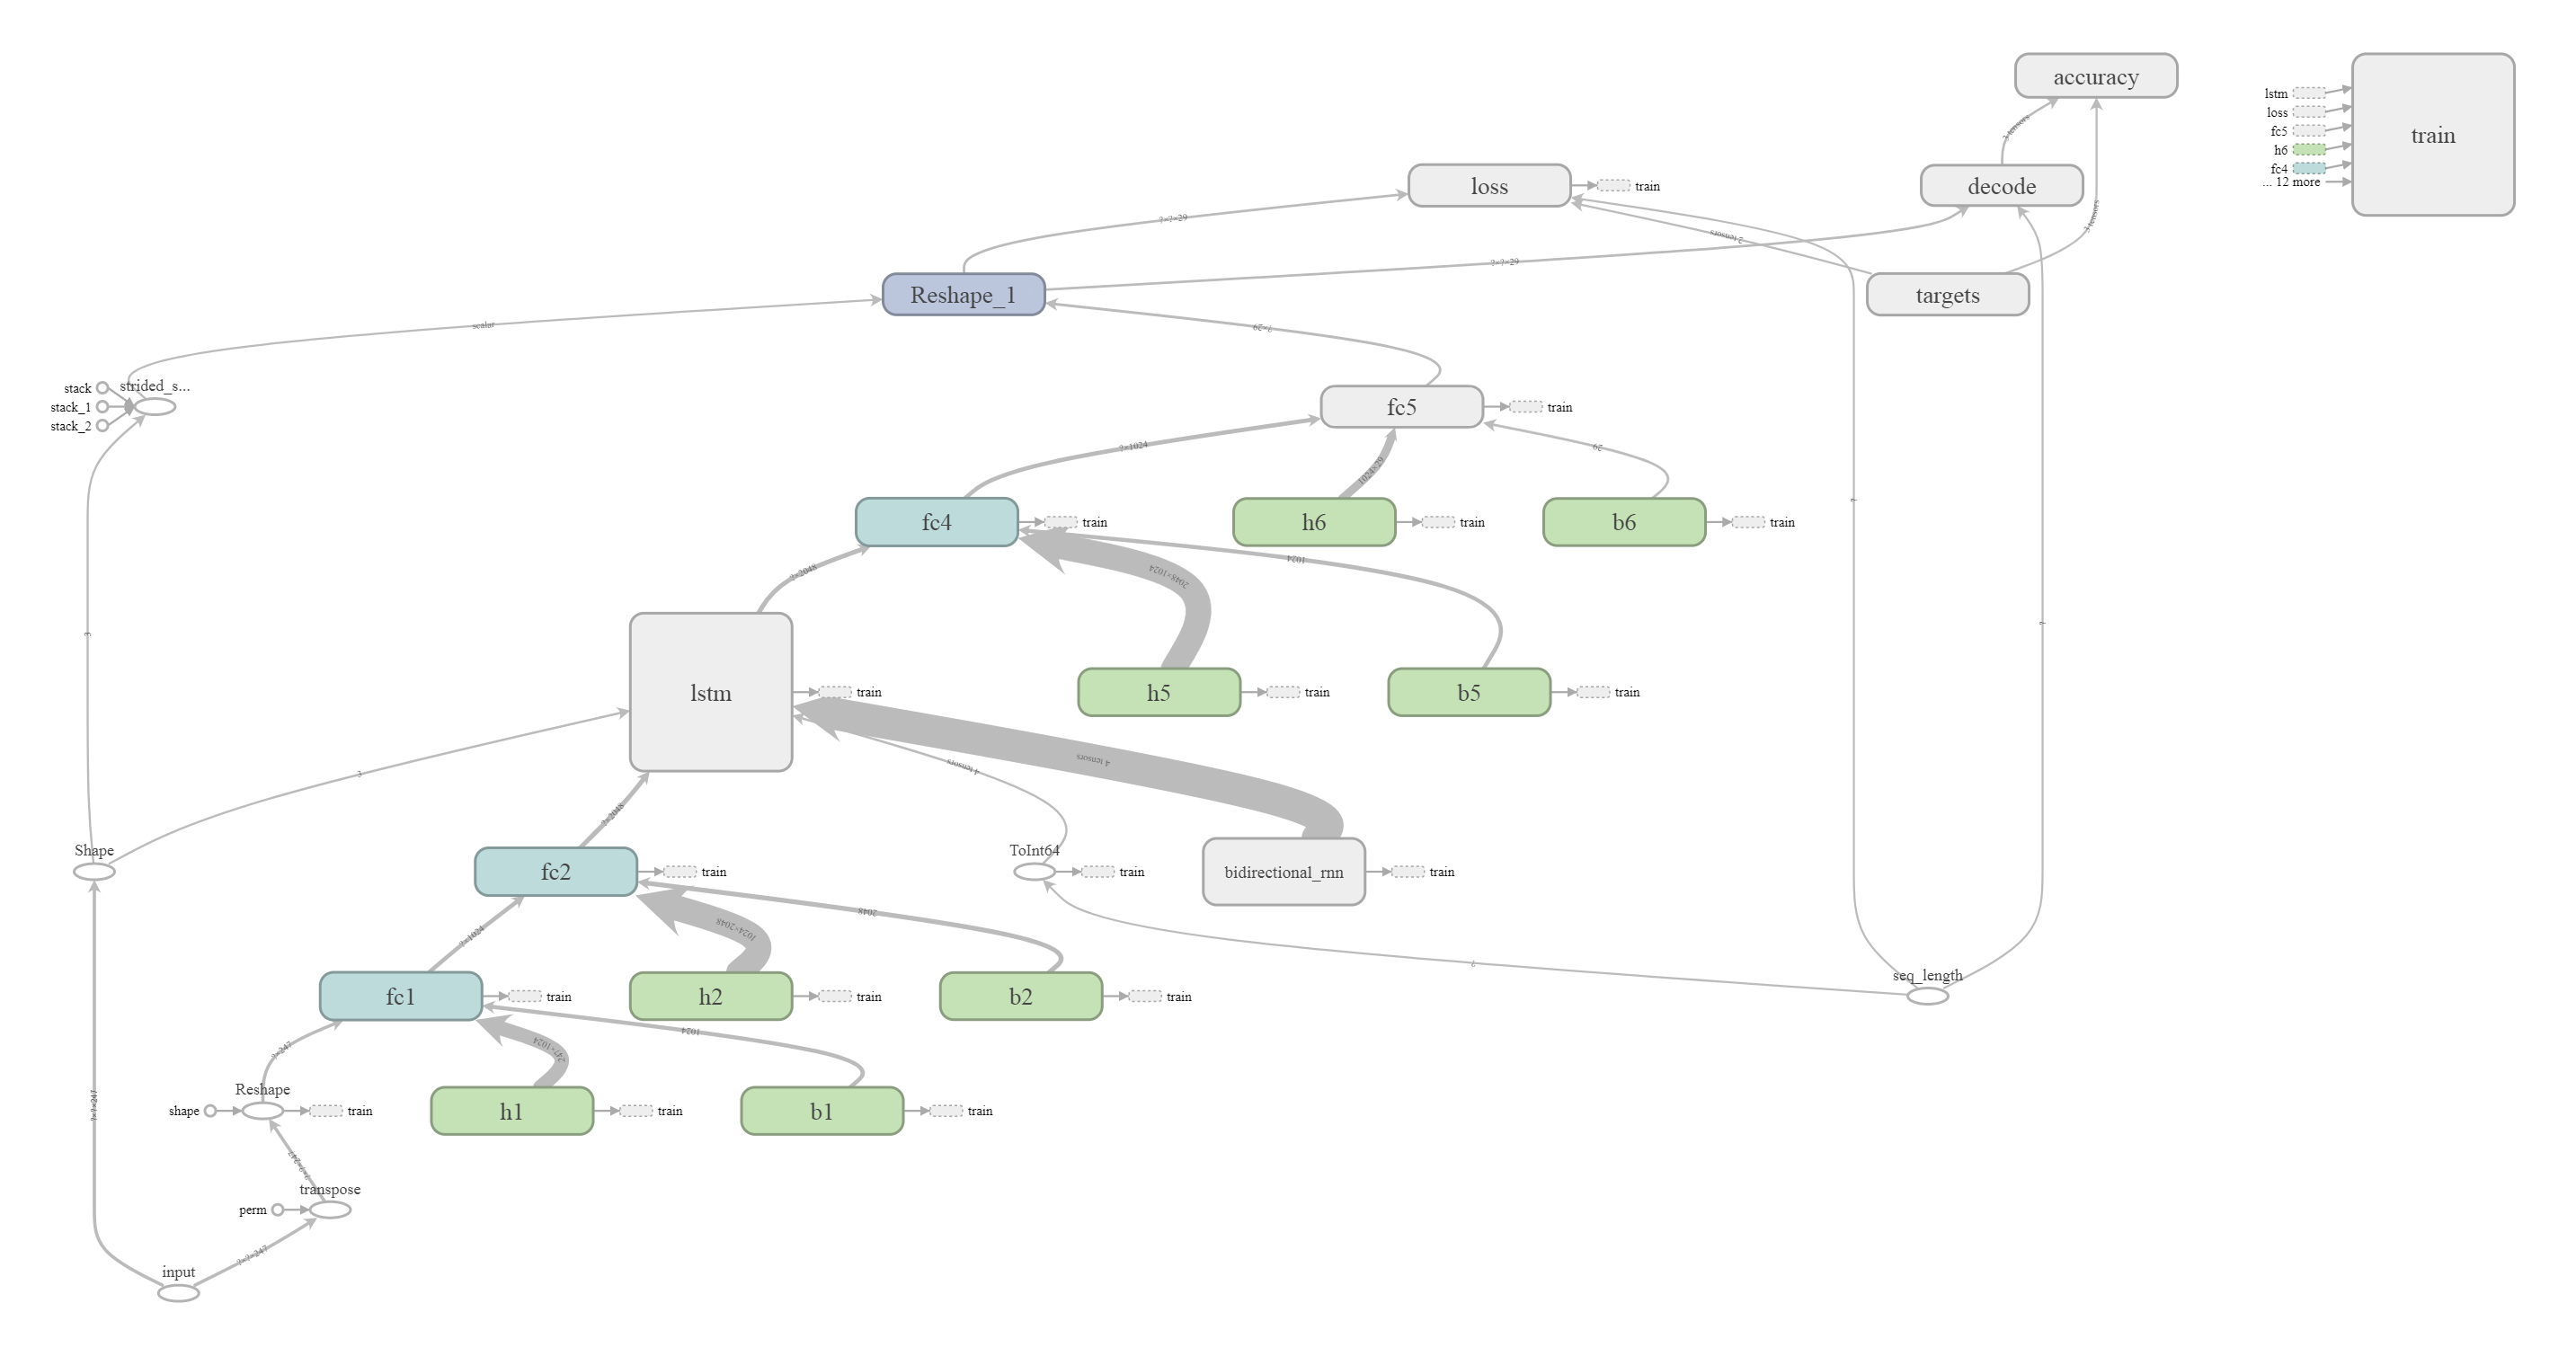
\includegraphics[width=\textwidth]		
	{model_development/birnn_v2_graph}
	\caption{Our BiRNN model graph.}
\end{figure}
Figure X shows the complete topology of the network used in the current implementation.
The structure is: 2-BiRNN-1-output.
In the beginning there are 2 fully connected layers, each consisting of 1024 neurons.\\
The first layer is designed to accept input from a 2D tensor. However, the input tensor has 3 dimensions.
To resolve this discrepancy, the input tensor is reshaped into a 2D representation. Two dimensions are merged, thus the 3D tensor becomes 2D, and is ready to be sent through the network.
After the multiplication, the activation function is applied. 
For this type of layer, ReLU activation is used. 
The last operation in the layer applies drop-out on the neurons.
To visualize elements over time, TensorFlow's TensorBoard utility is used, and various information is saved after every layer.
\lstinputlisting[language=Python,caption = First fully connected layer, firstline=657, lastline=667]{code/rnn.py}
The second layer has much of the same functionality as the first. However, they differ in the output dimension size, because the output of this layer is going to be the input for the bidirectional LSTM layer.
\lstinputlisting[language=Python,caption = Second fully connected layer, firstline=669, lastline=678]{code/rnn.py}
The next layer defines two LSTM cells. Both are initialised with the default forget bias, in order to remember more information at the beginning of training. For these cells there is no drop-out.
\lstinputlisting[language=Python,caption = BiRNN Layer, firstline=694, lastline=702]{code/rnn.py}
Further on, the input is reshaped into a three dimensional tensor, to be compatible with the BiRNN layer, and the network is unrolled. 
\lstinputlisting[language=Python,caption = BiRNN Layer, firstline=718, lastline=723]{code/rnn.py}
Following, the previous outputs is reshaped again into a 2 dimensional tensor, and sent to the next fully connected layer. 
This layer is similar to the first two, with the main operation being tensor multiplication and addition.
Afterwards, ReLU and drop-out is applied.
\lstinputlisting[language=Python,caption = Third fully connected layer, firstline=732, lastline=737]{code/rnn.py}
The output layer, is used as the end point of the network.
Multiplication and addition operations are applied to the previous output tensor. 
At this point, the output was  transformed by the entire network. 
The last step is to reshape the tensor back into a 3D form, after which it is passed to another function for decoding.
\lstinputlisting[language=Python,caption = Output layer, firstline=746, lastline=748]{code/rnn.py}
	
	\chapter{Implementation}\label{ch:implementation}

\section{Data Mining}
\subsubsection{Data Set}
Any neural network requires data in order to learn and become useful. As such, the training data is an important part of the learning process. For this implementation, the OpenSLR LibriSpeech ASR corpus was imported to provide training data.\\

The LibriSpeech is comprised of approximately 1000 hours of 16kHz English read speech in .flac format, and was prepared by Vassil Panayotov with the assistance of Daniel Povey. It is based on audio books from the LibriVox project that have been segmented and aligned. It contains 3 different sets, differentiated by type and size.\\ 
The first, and smallest one, is made of 6.3 GB of "clean" speech, representing approx. 100 hours. "Clean" speech refers to audio recordings where noise and disturbances that might corrupt their quality were eliminated as much as possible.\\ 
The second set is made of 23 GB of "clean" speech that represents approx. 360 hours.\\
The final set is made of 30 GB of "other" speech, representing approx. 500 hours of audio. "Other" speech refers to recordings that contain a certain degree of audio disturbance.\\
The corpus also contains smaller sets for validation and testing.\\

\subsubsection{Data processing}
As presented above, the OpenSLR corpus provides many features for training neural networks. It is especially efficient for speech recognition systems. However, the current implementation was designed to use pairs of .wav files and .txt files as input. Each .wav file represents the audio information that is encoded into the corresponding .txt file, more specifically short paragraphs.\\

Unfortunately, this data set is prepared in a different format. There is a single .txt file that corresponds to many .wav files and these are organized in bigger sets. Because of this, the data in its original form is not usable for the current neural network. To prepare the data, certain scripts were implemented in Python.\\

The first algorithm is designed to navigate a folder path and its sub-folders to convert all .flac files to .wav. It uses the os and pydub libraries.  \\
To access every sub-folder in the path, os.walk is used. This function returns the root folder and a list of files and directories in root. 

\lstinputlisting[language=Python, firstline=37, lastline=51]{code/FlacToWavPy.py}

The conversion is handled by another function that uses the pydub library to load the .flac, parse the name and   export the converted .wav file.

\lstinputlisting[language=Python, firstline=25, lastline=35]{code/FlacToWavPy.py}

The second algorithm navigates the folders in the same way, by using the os.walk method. Then it checks for .txt files by parsing their name. 

\lstinputlisting[language=Python, firstline=13, lastline=22]{code/txtFileMaker.py}

The format of the text files in this audio set is known. Using this information, the file name and content is parsed, creating new text files for every paragraph that corresponds to a flac file. This is achieved by exploiting the file name in relation to the beginning and end of each paragraph inside the file.
 
\lstinputlisting[language=Python, firstline=42, lastline=53]{code/txtFileMaker.py} 
 
\section{Model Implementation}






\section{Testing}











	
	\chapter{Discussion}\label{ch:discussion}

\section{Discussion}
In chapter two, specific success criteria were created to limit the scope and also allow for the project to be evaluated. This discussion will focus on what was accomplished in terms of success criteria and on the possible future steps to improve or advance this project. The list of success criteria from Section \ref{sec:PD}, Problem Delimitation is shown below:

\begin{itemize}
	\item Data mining
	\item Choose a filter
	\item Design a deep neural network model
	\item Train for the English language
	\item Create a Client/Server framework
	\item Implement the distributed model
\end{itemize} 

In order to use the OpenSLR training set, it was crucial to develop and use the 
scripts detailed in Section \ref{sec:DataMining}.
 Having an algorithm capable of following a path from a main folder and its sub-folders to convert all the necessary files to the right format meant that the 
 amount of data increased drastically.
  Using up to $1000$ hours of speech for the neural network to learn from was 
  crucial in the development phase. 
  As no network, no matter how complex and well thought out, could have a scope of 
  understanding the full English language from a limited data set. 
  Another important difference is to be made between clean speech and noisy speech, 
  as a network trained only with clean speech stands no chance in recognizing our 
  voices. 
  The preprocessing part covered in Chapter \ref{ch:speech_processing}, and more
   closely in Section \ref{sec:Modernanalysis}, was  successfully implemented by 
   using the 26 cepstrum coefficient to shape information to be fed to the first 
   layer of of neurons. With the MFC, the signal used as an input is converted to the frequency
   domain and distributed evenly on a scale mimicking the human ear. Without this step, the neural
   network wouldn't have been able to receive any input.\\
   
   For the main part, which consisted of the design and development of the neural network model, a reference model was originally used for understanding and testing. The Stanford model of a simple LSTM neural network proved to be a strong starting point for our own neural networks. As it was used to get acquainted to all the different dependencies and intricacies that these systems posses. By reverse engineering the reference model, we were able to construct a series of more complex and better performing networks.\\
    
   By trial and error, the first fully functional model that outperformed the Stanford model was described in Section \ref{sec:NNComparison}. The addition of fully connected layers both before and after the core LSTM layers proved to be an efficient way of reducing the word error rate across all the testing range, clearly seen in Figure \ref{fig:validation_error_fig}. A further analysis of the state-of-the-art neural networks developed specifically for understanding speech revealed that a BiRNN could prove to be a better solution to the classical stacking of LSTM layers. From the idea that hidden vectors can compute previous and future states, a second model was pursued, having a BiRNN layer as its core. Seen in Figure \ref{fig:BiRNNFC}, the best performing model is shown as a combination of FC and BiRNN. \\
   
Both models, LSTM and BiRNN were trained on the English language, by using the LibriSpeech set. To achieve this goal, a large number of parameters had to be tuned to ensure that the network didn't diverge during learning. As there is no predetermined way to set the parameters, training was done on an iterative process and the results were documented in Appendix \ref{ch:appClabel}.\\

The next step was to distribute the SR system. The server was established on the computer which had the video card and where the neural network was designed. This was done in order to assure that the server had enough processing power to complete the tasks sent by the users. Via the LAN network any client that has access to the SR system can send a wave file and receive a written text file containing the transcription of their voice. \\

\section{Future work}
For future development, a series of topics can be pursued for the 
betterment of the DSR.
 One of the key ideas pointed out in the report was that training data is 
 crucial for the system, and as such, a first addition should constitute in the creation of even larger data sets. 
 While a larger set of data will prove beneficial, sets that emulate real 
 life speech, such as speech in a noisy environment or multiple speakers 
 at the same time will greatly benefit the learning curve of any neural 
 network. The scope of this project was also limited by the hardware available 
 at the time of this research paper, with such considerations, more 
 powerful hardware will prove instrumental in reducing the processing time 
 and increasing the efficiency of writing and developing better neural 
 networks. Due to time constraints, a balance between the time that the 
 network was training and time the models were developed had to be 
 maintained. Moreover, data sets should be able to run 
 for increased amounts of time to reduce the word error rate even further. \\
 
 A major goal that can be achieved by building upon the results of this project is the creation of an information retrieval (IR) system. 
 As data is returned in text format to the client, an IR system can search 
 a predefined database, or use a web crawler to access specific web pages 
 and return meaningful snippets of information related to the predetermined interests of the user.

Another improvement would target the distribution part of the system. TensorFlow Serving is a flexible, high-performance serving system for machine learning models. It is designed for production environments, and it provides an easy way to deploy new algorithms and experiments, without changing the server architecture. Illustrated in \ref{fig:TFServe}. It would provide a great option for testing different models efficiently.

\begin{figure}[H]
	\centering
	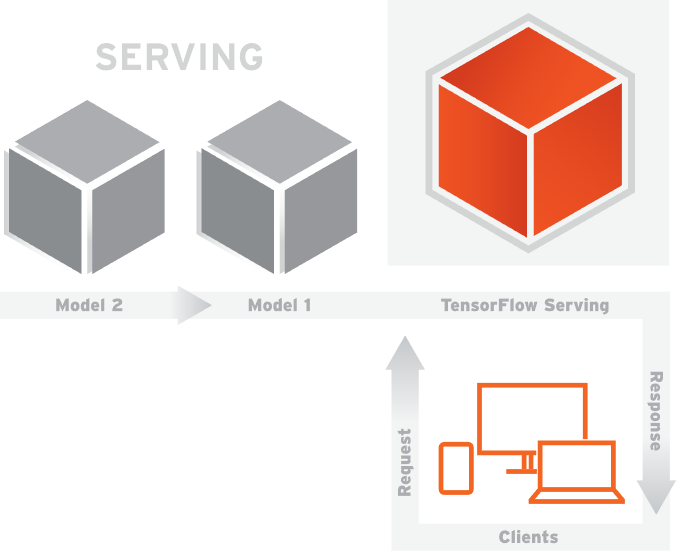
\includegraphics[width=.7\textwidth]		
	{future_work/TensorFlowServing}
	\caption{TensorFlow Serving \cite{TFServ}.}
	\label{fig:TFServe}
\end{figure}
	
	\chapter{Conclusion}\label{ch:conclusion}
In case you have questions, comments, suggestions or have found a bug, please do not hesitate to contact me. You can find my contact details below.
  \begin{center}
    Jesper Kjær Nielsen\\
    \href{mailto: jkn@es.aau.dk}{jkn@es.aau.dk}\\
    \href{http://kom.aau.dk/~jkn}{http://kom.aau.dk/\textasciitilde jkn}\\
    Fredrik Bajers Vej 7\\
    9220 Aalborg Ø
  \end{center}

	%---------------------------------------------------------%	
	\printbibliography[heading=bibintoc]
	\label{bib:mybiblio}
	
	\appendix
	\renewcommand\chaptername{Appendix}
	\chapter{MATLAB}\label{ch:appAlabel}
\section{Waveform, FFT and spectrogram script}
\begin{lstlisting}[language=Matlab, caption = MATLAB script.]
%--------------------------------------------------------
%Loading the "Hello" sample
subplot(3,1,1);
[y,Fs] = audioread('microphone-results.wav');
sound(y,Fs);
    dt = 1/Fs;
    t = 0:dt:(length(y)*dt)-dt;
    %figure();
    plot(t,y); xlabel('Seconds'); ylabel('Amplitude');
title('Hello waveform');
%--------------------------------------------------------
%Creating the FFT of the signal
subplot(3,1,2);
N = length(y);
NEFT = 2^nextpow2(N)
Xk=fft(y, NEFT)/N;                % perform N-point DFT of signal
fa = 8000/2*linspace(0,1,NEFT/2+1); 
%figure();
plot(fa, 2*abs(Xk(1:NEFT/2+1)));
title('FFT Spectrum Estimates / Power Spectral Density');
xlabel('Frequency Index'),
ylabel('Amplitude');
%--------------------------------------------------------
% Creating the Spectrogram
%figure();
subplot(3,1,3);
s = spectrogram(y);
spectrogram(y,'yaxis')
\end{lstlisting}

\begin{figure}[H]
	\centering
	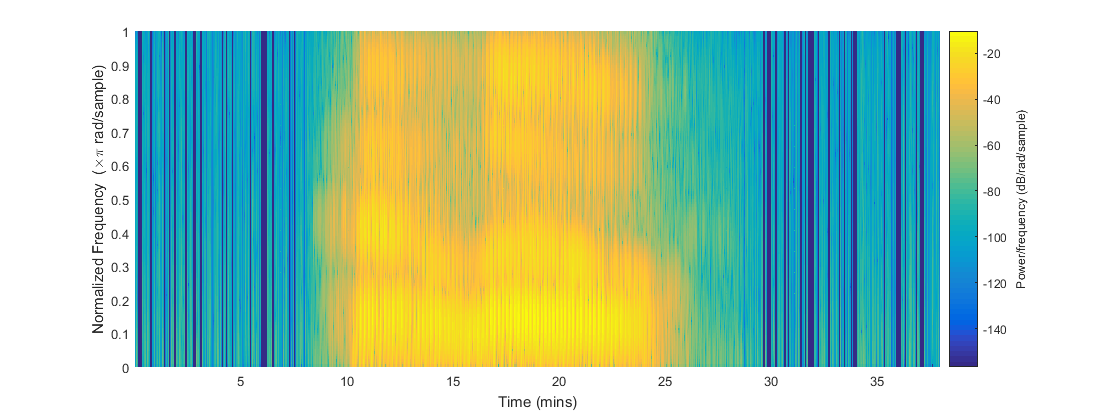
\includegraphics[width=\textwidth]		
	{speech_processing/04_Spectrogram}
	\caption{Spectrogram generated from FFT.}
	\label{fig:Spectrogram}
\end{figure}









	\chapter{Batch Size, Dropout and Learning Rate Comparison Data}\label{ch:appBlabel}

\section{Batch Size Test}
\subsubsection{Final table results}
%-------------------------------------------------------
\begin{table}[H]
\begin{minipage}{0.5\textwidth}
\centering
	\caption{Test error rate results.}
	\begin{tabular}{| l | c | c | c |}
	\hline
	Tests & Value & Epoch & Duration \\
	\hline
	Test1 -\tikzcircle[orange, fill=orange]{3pt}- &
	0.1308 & 25.00 & 0s\\
	\hline
	Test2 -\tikzcircle[blue, fill=blue]{3pt}- &
	0.000 & 25.00 & 0s\\
	\hline
	Test5 -\tikzcircle[pink, fill=pink]{3pt}- &
	0.000 & 25.00 & 0s\\
	\hline
	\end{tabular}
\end{minipage}
\begin{minipage}[c]{0.5\textwidth}
\centering
	\caption{Training error rate results.}
	\begin{tabular}{| l | c | c | c |}
	\hline
	Tests & Value & Epoch & Duration \\
	\hline
	Test1 -\tikzcircle[orange, fill=orange]{3pt}- &
	0.1148 & 24.00 & 1h 26m 13s\\
	\hline
	Test2 -\tikzcircle[blue, fill=blue]{3pt}- &
	9.5073e-4 & 24.00 & 18m 50s\\
	\hline
	Test5 -\tikzcircle[pink, fill=pink]{3pt}- &
	5.1858e-4 & 24.00 & 14m 50s\\
	\hline
	\end{tabular}
\end{minipage}%
\end{table}
\begin{table}[H]
\begin{minipage}{0.52\textwidth}
\centering
	\caption{Validation error rate results.}
	\begin{tabular}{| l | c | c | c |}
	\hline
	Tests & Value & Epoch & Duration \\
	\hline
	Test1 -\tikzcircle[orange, fill=orange]{3pt}- &
	0.1608 & 23.00 & 1h 15m 58s\\
	\hline
	Test2 -\tikzcircle[blue, fill=blue]{3pt}- &
	0.05887 & 23.00 & 17m 21s\\
	\hline
	Test5 -\tikzcircle[pink, fill=pink]{3pt}- &
	0.05418 & 23.00 & 13m 50s\\
	\hline
	\end{tabular}
\end{minipage}
\begin{minipage}[c]{0.5\textwidth}
\centering
	\caption{Training average loss results.}
	\begin{tabular}{| l | c | c | c |}
	\hline
	Tests & Value & Epoch & Duration \\
	\hline
	Test1 -\tikzcircle[orange, fill=orange]{3pt}- &
	1.639 & 24.00 & 1h 26m 13s\\
	\hline
	Test2 -\tikzcircle[blue, fill=blue]{3pt}- &
	0.06023 & 24.00 & 18m 50s\\
	\hline
	Test5 -\tikzcircle[pink, fill=pink]{3pt}- &
	0.01988 & 24.00 & 14m 50s\\
	\hline
	\end{tabular}
\end{minipage}%
\end{table}
\begin{figure}[H]
    \centering
    \begin{minipage}{0.5\textwidth}
        \centering
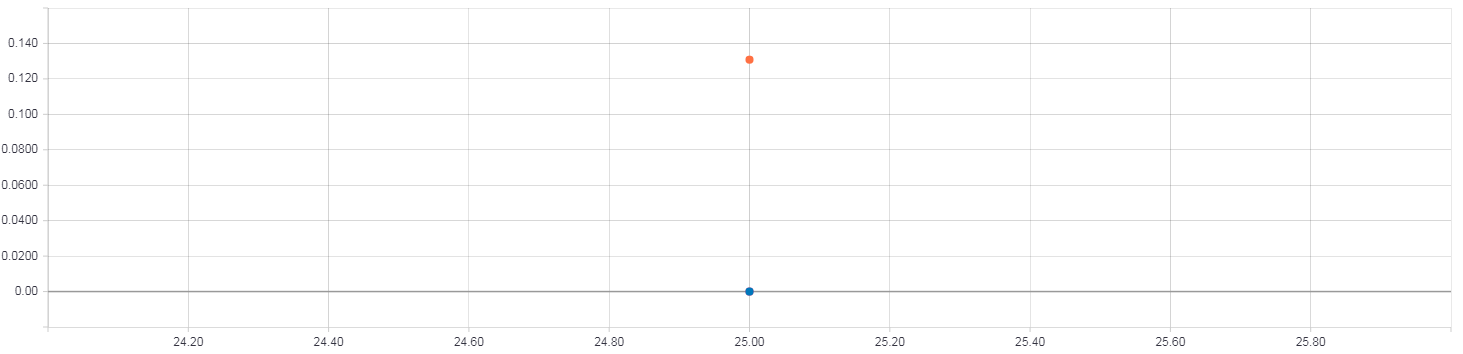
\includegraphics[width=3\textwidth, angle=90]		
	{machine_learning/graph_tests/batch_test/test_error_rate}
        \caption{Test error rate.}
    \end{minipage}\hfill
    \begin{minipage}{0.5\textwidth}
        \centering
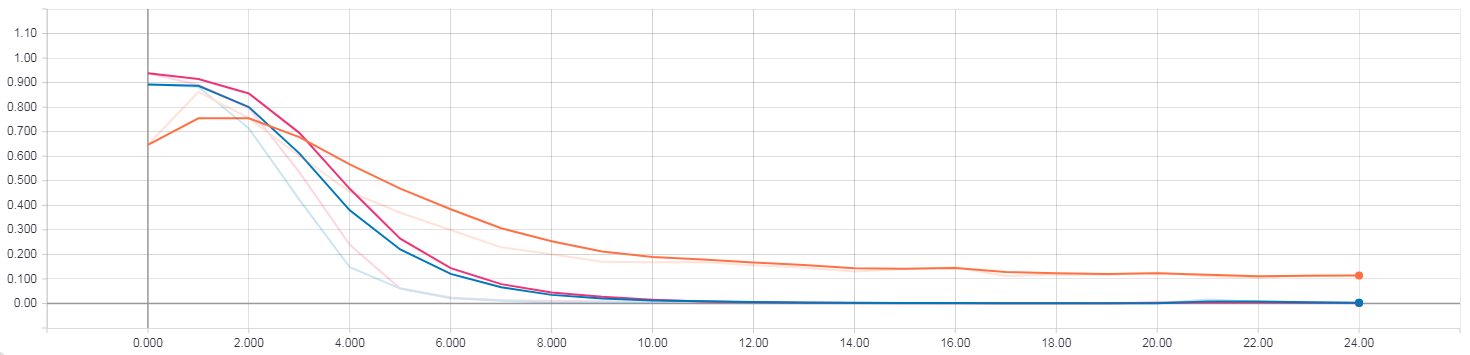
\includegraphics[width=3\textwidth, angle=90]	
	{machine_learning/graph_tests/batch_test/train_error_rate}
        \caption{Training error rate.}
    \end{minipage}
\end{figure}
\begin{figure}[H]
    \centering
    \begin{minipage}{0.5\textwidth}
        \centering
	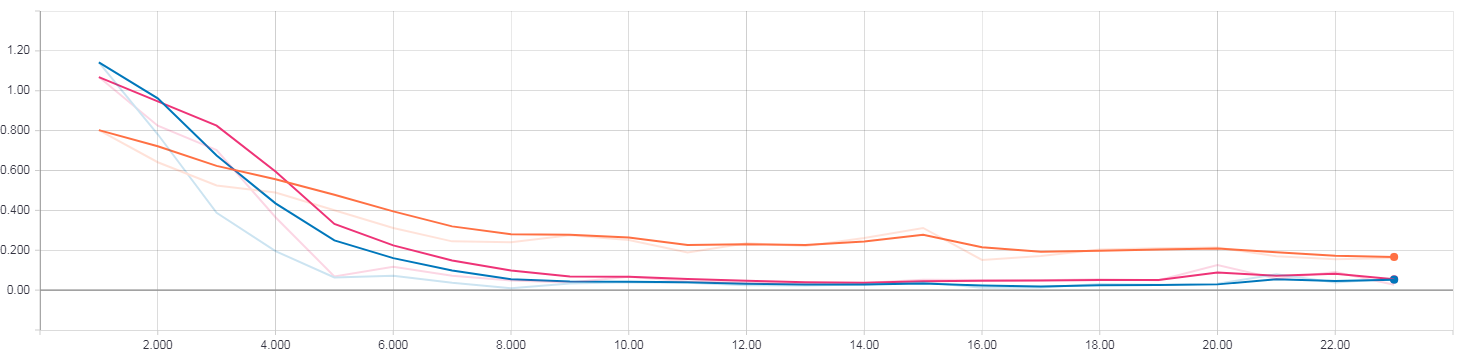
\includegraphics[width=3\textwidth, angle=90]		
	{machine_learning/graph_tests/batch_test/validation_error_rate}
        \caption{Validation error rate.}
    \end{minipage}\hfill
    \begin{minipage}{0.5\textwidth}
        \centering
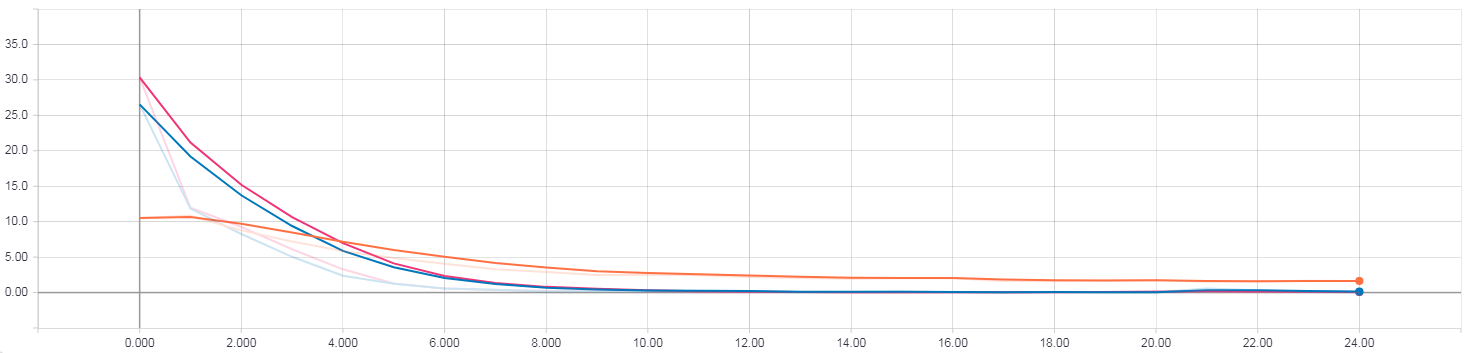
\includegraphics[width=3\textwidth, angle=90]		
	{machine_learning/graph_tests/batch_test/train_avg_loss}
        \caption{Training average loss.}
    \end{minipage}
\end{figure}

%%test error rate
%\begin{figure}[H]
%\centering
%	\includegraphics[width=\textwidth]		
%	{machine_learning/graph_tests/batch_test/test_error_rate}
%	\caption{Test error rate.}
%\end{figure}
%%training error rate
%\begin{figure}[H]
%	\centering
%	\includegraphics[width=\textwidth]		
%	{machine_learning/graph_tests/batch_test/train_error_rate}
%	\caption{Training error rate.}
%\end{figure}
%%validation error rate
%\begin{figure}[H]
%	\centering
%	\includegraphics[width=\textwidth]		
%	{machine_learning/graph_tests/batch_test/validation_error_rate}
%	\caption{Validation error rate.}
%\end{figure}
%%training average loss
%\begin{figure}[H]
%	\centering
%	\includegraphics[width=\textwidth]		
%	{machine_learning/graph_tests/batch_test/train_avg_loss}
%	\caption{Training average loss.}
%\end{figure}
%\begin{table}[H]
%\centering
%	\caption{Test error rate results.}
%	\begin{tabular}{| l | c | c | c |}
%	\hline
%	Tests & Value & Epoch & Duration \\
%	\hline
%	Test1 -\tikzcircle[orange, fill=orange]{3pt}- &
%	0.1308 & 25.00 & 0s\\
%	\hline
%	Test2 -\tikzcircle[blue, fill=blue]{3pt}- &
%	0.000 & 25.00 & 0s\\
%	\hline
%	Test5 -\tikzcircle[pink, fill=pink]{3pt}- &
%	0.000 & 25.00 & 0s\\
%	\hline
%	\end{tabular}
%\end{table}
%\begin{table}[H]
%\centering
%	\caption{Training error rate results.}
%	\begin{tabular}{| l | c | c | c |}
%	\hline
%	Tests & Value & Epoch & Duration \\
%	\hline
%	Test1 -\tikzcircle[orange, fill=orange]{3pt}- &
%	0.1148 & 24.00 & 1h 26m 13s\\
%	\hline
%	Test2 -\tikzcircle[blue, fill=blue]{3pt}- &
%	9.5073e-4 & 24.00 & 18m 50s\\
%	\hline
%	Test5 -\tikzcircle[pink, fill=pink]{3pt}- &
%	5.1858e-4 & 24.00 & 14m 50s\\
%	\hline
%	\end{tabular}
%\end{table}
%\begin{table}[H]
%\centering
%	\caption{Validation error rate results.}
%	\begin{tabular}{| l | c | c | c |}
%	\hline
%	Tests & Value & Epoch & Duration \\
%	\hline
%	Test1 -\tikzcircle[orange, fill=orange]{3pt}- &
%	0.1608 & 23.00 & 1h 15m 58s\\
%	\hline
%	Test2 -\tikzcircle[blue, fill=blue]{3pt}- &
%	0.05887 & 23.00 & 17m 21s\\
%	\hline
%	Test5 -\tikzcircle[pink, fill=pink]{3pt}- &
%	0.05418 & 23.00 & 13m 50s\\
%	\hline
%	\end{tabular}
%\end{table}
%\begin{table}[H]
%\centering
%	\caption{Training average loss results.}
%	\begin{tabular}{| l | c | c | c |}
%	\hline
%	Tests & Value & Epoch & Duration \\
%	\hline
%	Test1 -\tikzcircle[orange, fill=orange]{3pt}- &
%	1.639 & 24.00 & 1h 26m 13s\\
%	\hline
%	Test2 -\tikzcircle[blue, fill=blue]{3pt}- &
%	0.06023 & 24.00 & 18m 50s\\
%	\hline
%	Test5 -\tikzcircle[pink, fill=pink]{3pt}- &
%	0.01988 & 24.00 & 14m 50s\\
%	\hline
%	\end{tabular}
%\end{table}	
%-------------------------------------------------------
\section{Dropout Test}
\subsubsection{Final table results}
\begin{table}[H]
\begin{minipage}{0.5\textwidth}
\centering
	\caption{Test error rate results.}
	\begin{tabular}{| l | c | c | c |}
	\hline
	Tests & Value & Epoch & Duration \\
	\hline
	Test2 -\tikzcircle[blue, fill=blue]{3pt}- &
	0.000 & 25.00 & 0s\\
	\hline
	Test3 -\tikzcircle[red, fill=red]{3pt}- &
	0.030 & 25.00 & 0s\\
	\hline
	Test4 -\tikzcircle[lightblue, fill=lightblue]{3pt}- &
	0.020 & 25.00 & 0s\\
	\hline
	\end{tabular}
\end{minipage}
\begin{minipage}[c]{0.5\textwidth}
\centering
\caption{Training error rate results.}
	\begin{tabular}{| l | c | c | c |}
	\hline
	Tests & Value & Epoch & Duration \\
	\hline
	Test2 -\tikzcircle[blue, fill=blue]{3pt}- &
	9.5973e-4 & 24.00 & 18m 50s\\
	\hline
	Test3 -\tikzcircle[red, fill=red]{3pt}- &
	0.000 & 24.00 & 18m 5s\\
	\hline
	Test4 -\tikzcircle[lightblue, fill=lightblue]{3pt}- &
	6.3331e-3 & 24.00 & 18m 10s\\
	\hline
	\end{tabular}
\end{minipage}%
\end{table}
\begin{table}[H]
\begin{minipage}{0.52\textwidth}
\centering
	\caption{Validation error rate results.}
	\begin{tabular}{| l | c | c | c |}
	\hline
	Tests & Value & Epoch & Duration \\
	\hline
	Test2 -\tikzcircle[blue, fill=blue]{3pt}- &
	0.05887 & 23.00 & 17m 21s\\
	\hline
	Test3 -\tikzcircle[red, fill=red]{3pt}- &
	0.05161 & 23.00 & 16m 36s\\
	\hline
	Test4 -\tikzcircle[lightblue, fill=lightblue]{3pt}- &
	0.02366 & 23.00 & 16m 35s\\
	\hline
	\end{tabular}
\end{minipage}
\begin{minipage}[c]{0.5\textwidth}
\centering
	\caption{Training average loss results.}
	\begin{tabular}{| l | c | c | c |}
	\hline
	Tests & Value & Epoch & Duration \\
	\hline
	Test2 -\tikzcircle[blue, fill=blue]{3pt}- &
	0.06023 & 24.00 & 18m 50s\\
	\hline
	Test3 -\tikzcircle[red, fill=red]{3pt}- &
	3.5483e-4 & 24.00 & 18m 5s\\
	\hline
	Test4 -\tikzcircle[lightblue, fill=lightblue]{3pt}- &
	0.09217 & 24.00 & 18m 10s\\
	\hline
	\end{tabular}
\end{minipage}%
\end{table}
\begin{figure}[H]
    \centering
    \begin{minipage}{0.5\textwidth}
        \centering
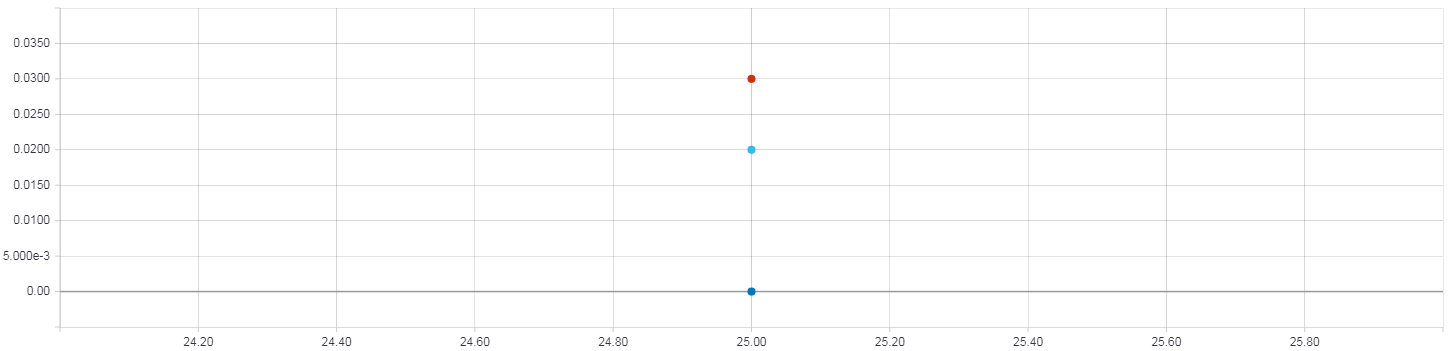
\includegraphics[width=3\textwidth, angle=90]		
	{machine_learning/graph_tests/dropout_test/test_error_rate}
        \caption{Test error rate.}
    \end{minipage}\hfill
    \begin{minipage}{0.5\textwidth}
        \centering
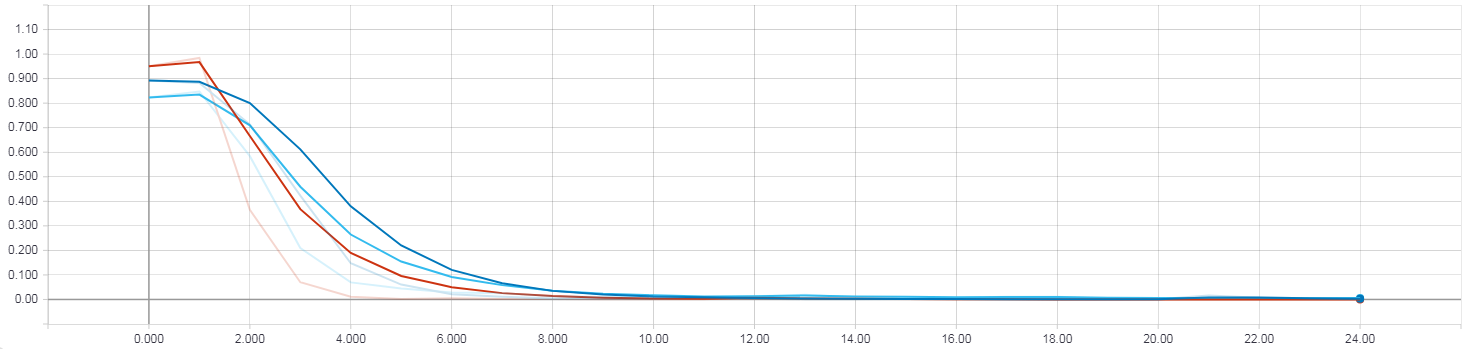
\includegraphics[width=3\textwidth, angle=90]	
	{machine_learning/graph_tests/dropout_test/train_error_rate}
        \caption{Training error rate.}
    \end{minipage}
\end{figure}
\begin{figure}[H]

    \centering
    \begin{minipage}{0.5\textwidth}
        \centering
	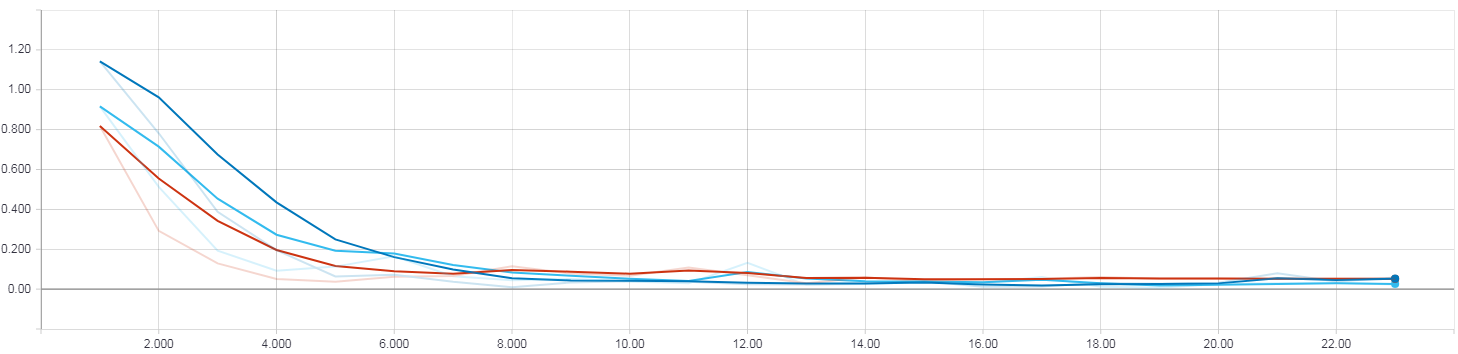
\includegraphics[width=3\textwidth, angle=90]		
	{machine_learning/graph_tests/dropout_test/validation_error_rate}
        \caption{Validation error rate.}
    \end{minipage}\hfill
    \begin{minipage}{0.5\textwidth}
        \centering
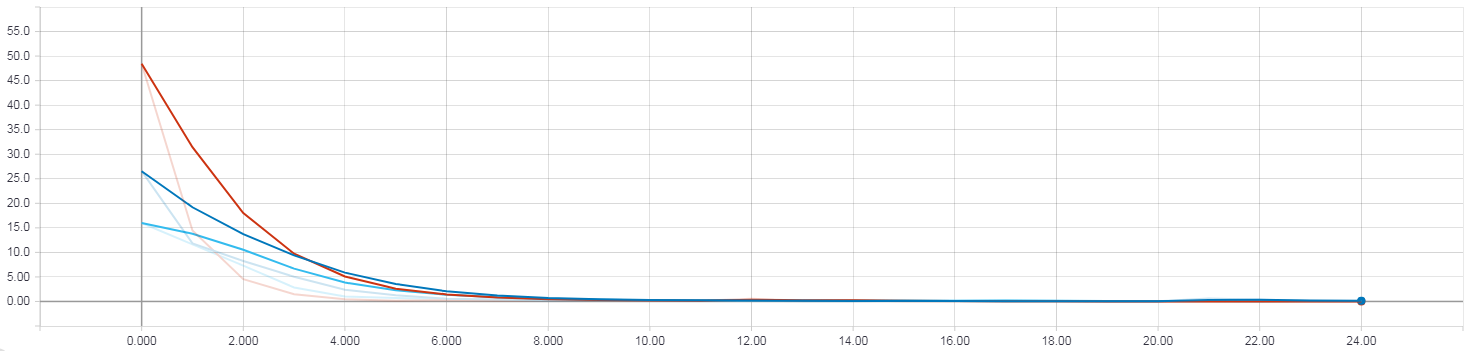
\includegraphics[width=3\textwidth, angle=90]		
	{machine_learning/graph_tests/dropout_test/train_avg_loss}
        \caption{Training average loss.}
    \end{minipage}
\end{figure}
%%test error rate
%\begin{figure}[H]
%	\centering
%	\includegraphics[width=\textwidth]		
%	{machine_learning/graph_tests/dropout_test/test_error_rate}
%	\caption{Test error rate.}
%\end{figure}
%%training error rate
%\begin{figure}[H]
%	\centering
%	\includegraphics[width=\textwidth]		
%	{machine_learning/graph_tests/dropout_test/train_error_rate}
%	\caption{Training error rate.}
%\end{figure}	
%%validation error rate
%\begin{figure}[H]
%	\centering
%	\includegraphics[width=\textwidth]		
%	{machine_learning/graph_tests/dropout_test/validation_error_rate}
%	\caption{Validation error rate.}
%\end{figure}
%%training avarage loss
%\begin{figure}[H]
%	\centering
%	\includegraphics[width=\textwidth]		
%	{machine_learning/graph_tests/dropout_test/train_avg_loss}
%	\caption{Training average loss.}
%\end{figure}	%-----------------------------------------------------
%\begin{table}[H]
%\centering
%	\caption{Test error rate results.}
%	\begin{tabular}{| l | c | c | c |}
%	\hline
%	Tests & Value & Epoch & Duration \\
%	\hline
%	Test2 -\tikzcircle[blue, fill=blue]{3pt}- &
%	0.000 & 25.00 & 0s\\
%	\hline
%	Test3 -\tikzcircle[red, fill=red]{3pt}- &
%	0.030 & 25.00 & 0s\\
%	\hline
%	Test4 -\tikzcircle[lightblue, fill=lightblue]{3pt}- &
%	0.020 & 25.00 & 0s\\
%	\hline
%	\end{tabular}
%\end{table}	
%\begin{table}[H]
%\centering
%	\caption{Training error rate results.}
%	\begin{tabular}{| l | c | c | c |}
%	\hline
%	Tests & Value & Epoch & Duration \\
%	\hline
%	Test2 -\tikzcircle[blue, fill=blue]{3pt}- &
%	9.5973e-4 & 24.00 & 18m 50s\\
%	\hline
%	Test3 -\tikzcircle[red, fill=red]{3pt}- &
%	0.000 & 24.00 & 18m 5s\\
%	\hline
%	Test4 -\tikzcircle[lightblue, fill=lightblue]{3pt}- &
%	6.3331e-3 & 24.00 & 18m 10s\\
%	\hline
%	\end{tabular}
%\end{table}	
%\begin{table}[H]
%\centering
%	\caption{Validation error rate results.}
%	\begin{tabular}{| l | c | c | c |}
%	\hline
%	Tests & Value & Epoch & Duration \\
%	\hline
%	Test2 -\tikzcircle[blue, fill=blue]{3pt}- &
%	0.05887 & 23.00 & 17m 21s\\
%	\hline
%	Test3 -\tikzcircle[red, fill=red]{3pt}- &
%	0.05161 & 23.00 & 16m 36s\\
%	\hline
%	Test4 -\tikzcircle[lightblue, fill=lightblue]{3pt}- &
%	0.02366 & 23.00 & 16m 35s\\
%	\hline
%	\end{tabular}
%\end{table}	
%\begin{table}[H]
%\centering
%	\caption{Training average loss results.}
%	\begin{tabular}{| l | c | c | c |}
%	\hline
%	Tests & Value & Epoch & Duration \\
%	\hline
%	Test2 -\tikzcircle[blue, fill=blue]{3pt}- &
%	0.06023 & 24.00 & 18m 50s\\
%	\hline
%	Test3 -\tikzcircle[red, fill=red]{3pt}- &
%	3.5483e-4 & 24.00 & 18m 5s\\
%	\hline
%	Test4 -\tikzcircle[lightblue, fill=lightblue]{3pt}- &
%	0.09217 & 24.00 & 18m 10s\\
%	\hline
%	\end{tabular}
%\end{table}	
%-----------------------------------------------------

\section{Learning Rate Test}
\subsubsection{Final table results}
\begin{table}[H]
\begin{minipage}{0.5\textwidth}
\centering
	\caption{Test error rate results.}
	\begin{tabular}{| l | c | c | c |}
	\hline
	Tests & Value & Epoch & Duration \\
	\hline
	Test5 -\tikzcircle[pink, fill=pink]{3pt}- &
	0.000 & 25.00 & 0s\\
	\hline
	Test6 -\tikzcircle[turquoise, fill=turquoise]{3pt}- &
	0.8992 & 25.00 & 0s\\
	\hline
	\end{tabular}
\end{minipage}
\begin{minipage}[c]{0.5\textwidth}
\centering
	\caption{Training error rate results.}
	\begin{tabular}{| l | c | c | c |}
	\hline
	Tests & Value & Epoch & Duration \\
	\hline
	Test5 -\tikzcircle[pink, fill=pink]{3pt}- &
	5.1858e-4 & 24.00 & 14m 50s\\
	\hline
	Test6 -\tikzcircle[turquoise, fill=turquoise]{3pt}- &
	0.9188 & 24.00 & 12m 29s\\
	\hline
	\end{tabular}
\end{minipage}%
\end{table}
\begin{table}[H]
\begin{minipage}{0.52\textwidth}
\centering
	\caption{Validation error rate results.}
	\begin{tabular}{| l | c | c | c |}
	\hline
	Tests & Value & Epoch & Duration \\
	\hline
	Test5 -\tikzcircle[pink, fill=pink]{3pt}- &
	0.02661 & 23.00 & 13m 50s\\
	\hline
	Test6 -\tikzcircle[turquoise, fill=turquoise]{3pt}- &
	1.152 & 23.00 & 11m 29s\\
	\hline
	\end{tabular}
\end{minipage}
\begin{minipage}[c]{0.5\textwidth}
\centering
	\caption{Training average loss results.}
	\begin{tabular}{| l | c | c | c |}
	\hline
	Tests & Value & Epoch & Duration \\
	\hline
	Test5 -\tikzcircle[pink, fill=pink]{3pt}- &
	0.01988 & 24.00 & 14m 50s\\
	\hline
	Test6 -\tikzcircle[turquoise, fill=turquoise]{3pt}- &
	12.56 & 24.00 & 12m 29s\\
	\hline
	\end{tabular}
\end{minipage}%
\end{table}
\begin{figure}[H]
    \centering
    \begin{minipage}{0.5\textwidth}
        \centering
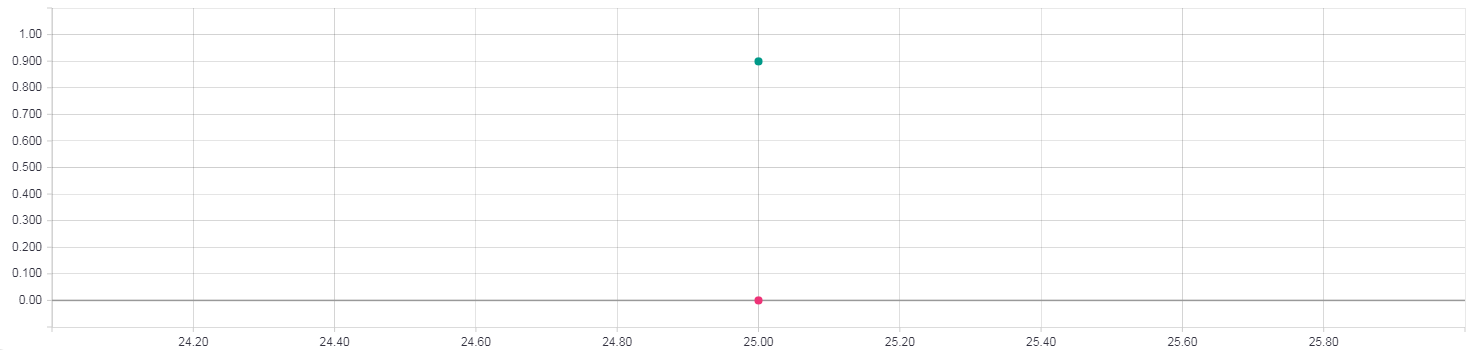
\includegraphics[width=3\textwidth, angle=90]		
	{machine_learning/graph_tests/learning_rate_test/test_error_rate}
        \caption{Test error rate.}
    \end{minipage}\hfill
    \begin{minipage}{0.5\textwidth}
        \centering
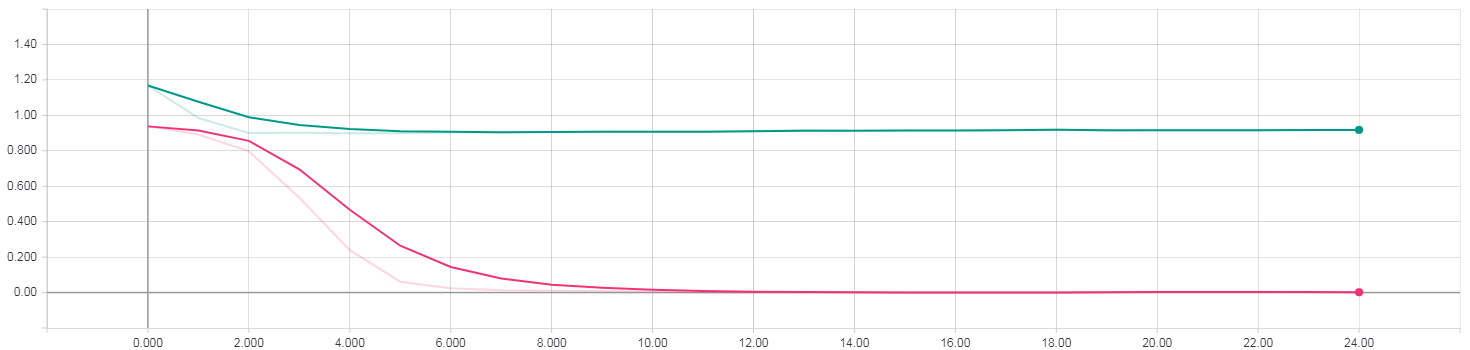
\includegraphics[width=3\textwidth, angle=90]	
	{machine_learning/graph_tests/learning_rate_test/train_error_rate}
        \caption{Training error rate.}
    \end{minipage}
\end{figure}
\begin{figure}[H]
    \centering
    \begin{minipage}{0.5\textwidth}
        \centering
	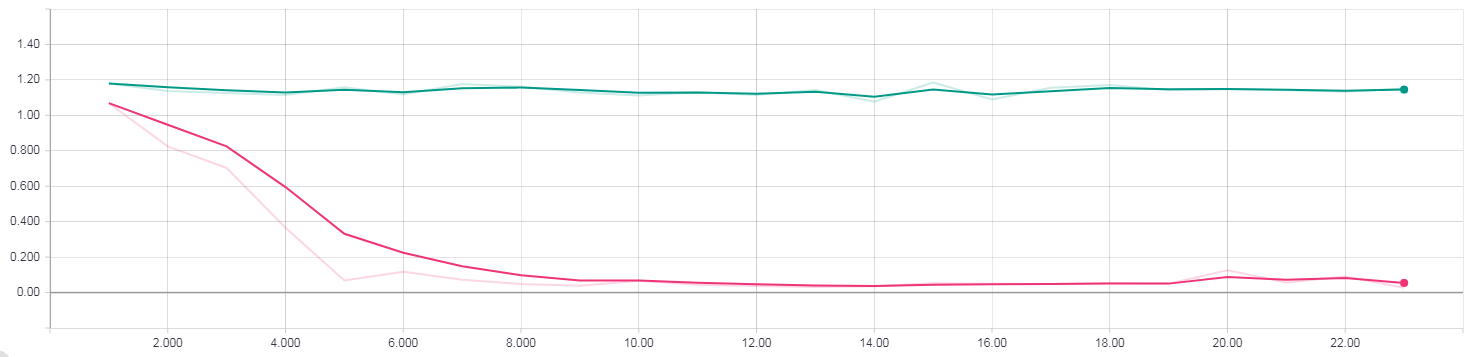
\includegraphics[width=3\textwidth, angle=90]		
	{machine_learning/graph_tests/learning_rate_test/validation_error_rate}
        \caption{Validation error rate.}
    \end{minipage}\hfill
    \begin{minipage}{0.5\textwidth}
        \centering
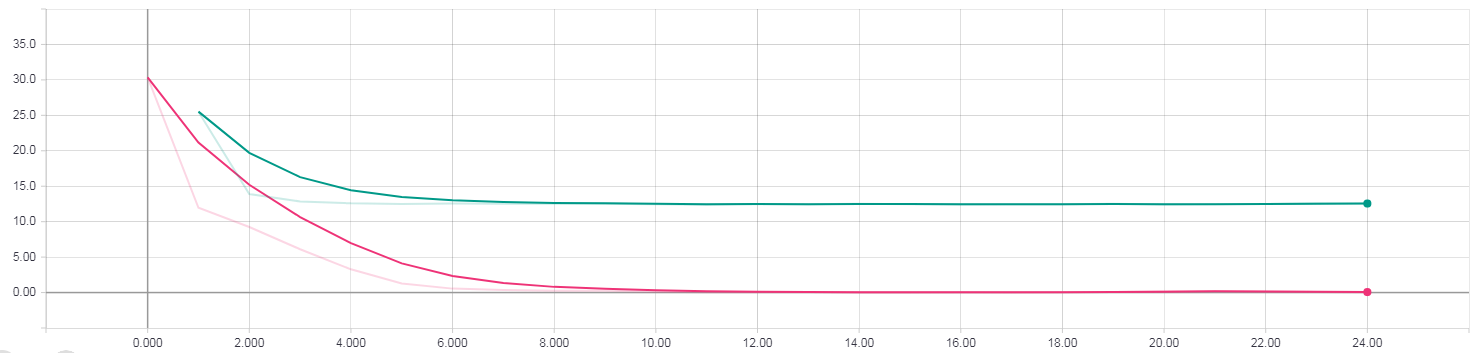
\includegraphics[width=3\textwidth, angle=90]		
	{machine_learning/graph_tests/learning_rate_test/train_avg_loss}
        \caption{Training average loss.}
    \end{minipage}
\end{figure}

%%test error rate
%\begin{figure}[H]
%	\centering
%	\includegraphics[width=\textwidth]		
%	{machine_learning/graph_tests/learning_rate_test/test_error_rate}
%	\caption{Test error rate.}
%\end{figure}
%%training error rate
%\begin{figure}[H]
%	\centering
%	\includegraphics[width=\textwidth]		
%	{machine_learning/graph_tests/learning_rate_test/train_error_rate}
%	\caption{Training error rate.}
%\end{figure}
%%validation error rate
%\begin{figure}[H]
%	\centering
%	\includegraphics[width=\textwidth]		
%	{machine_learning/graph_tests/learning_rate_test/validation_error_rate}
%	\caption{Validation error rate.}
%\end{figure}	
%%training avarage loss
%\begin{figure}[H]
%	\centering
%	\includegraphics[width=\textwidth]		
%	{machine_learning/graph_tests/learning_rate_test/train_avg_loss}
%	\caption{Training average loss.}
%\end{figure}
%\begin{table}[H]
%\centering
%	\caption{Test error rate results.}
%	\begin{tabular}{| l | c | c | c |}
%	\hline
%	Tests & Value & Epoch & Duration \\
%	\hline
%	Test5 -\tikzcircle[pink, fill=pink]{3pt}- &
%	0.000 & 25.00 & 0s\\
%	\hline
%	Test6 -\tikzcircle[turquoise, fill=turquoise]{3pt}- &
%	0.8992 & 25.00 & 0s\\
%	\hline
%	\end{tabular}
%\end{table}	
%\begin{table}[H]
%\centering
%	\caption{Training error rate results.}
%	\begin{tabular}{| l | c | c | c |}
%	\hline
%	Tests & Value & Epoch & Duration \\
%	\hline
%	Test5 -\tikzcircle[pink, fill=pink]{3pt}- &
%	5.1858e-4 & 24.00 & 14m 50s\\
%	\hline
%	Test6 -\tikzcircle[turquoise, fill=turquoise]{3pt}- &
%	0.9188 & 24.00 & 12m 29s\\
%	\hline
%	\end{tabular}
%\end{table}	
%\begin{table}[H]
%\centering
%	\caption{Validation error rate results.}
%	\begin{tabular}{| l | c | c | c |}
%	\hline
%	Tests & Value & Epoch & Duration \\
%	\hline
%	Test5 -\tikzcircle[pink, fill=pink]{3pt}- &
%	0.02661 & 23.00 & 13m 50s\\
%	\hline
%	Test6 -\tikzcircle[turquoise, fill=turquoise]{3pt}- &
%	1.152 & 23.00 & 11m 29s\\
%	\hline
%	\end{tabular}
%\end{table}	
%\begin{table}[H]
%\centering
%	\caption{Training average loss results.}
%	\begin{tabular}{| l | c | c | c |}
%	\hline
%	Tests & Value & Epoch & Duration \\
%	\hline
%	Test5 -\tikzcircle[pink, fill=pink]{3pt}- &
%	0.01988 & 24.00 & 14m 50s\\
%	\hline
%	Test6 -\tikzcircle[turquoise, fill=turquoise]{3pt}- &
%	12.56 & 24.00 & 12m 29s\\
%	\hline
%	\end{tabular}
%\end{table}		

	\chapter{Model Development Comparison Data}\label{ch:appClabel}


\begin{table}[H]
\centering
	\caption{Models.}
	\begin{tabular}{ l  c }
	Model1 -\tikzcircle[pink, fill=pink]{3pt}- &
	(Their simpleLSTM Model)\\
	Model2 -\tikzcircle[red, fill=red]{3pt}- &
	(Our simpleLSTM Model)\\
	Model3 -\tikzcircle[turquoise, fill=turquoise]{3pt}- &
	(Our BiRNN Model)\\
	\end{tabular}
	\label{tab:3_models}
\end{table}


\begin{table}[H]
\centering
    \caption{Parameter values of the three model.}
    \begin{tabular}{| l | c | c | c | c |} 
    \hline
        Parameters & 
        Model1 -\tikzcircle[pink, fill=pink]{3pt}- &
        Model2 -\tikzcircle[red, fill=red]{3pt}- &
        Model3 -\tikzcircle[turquoise, fill=turquoise]{3pt}-\\
    \hline
        Batch Size & 
        50 \hfill 20 \hfill 20 & 
        50 \hfill 20 \hfill 20 & 
        50 \hfill 20 \hfill 20 \\
    \hline
        Dropout & 
        0.05 & 0.05 & 0.05 \\
    \hline
        Learning Rate & 
        0.001 & 0.001 & 0.001 \\ 
    \hline
    \end{tabular}
    \label{tab:3models_tab}
\end{table}

\begin{figure}[H]
	\centering
	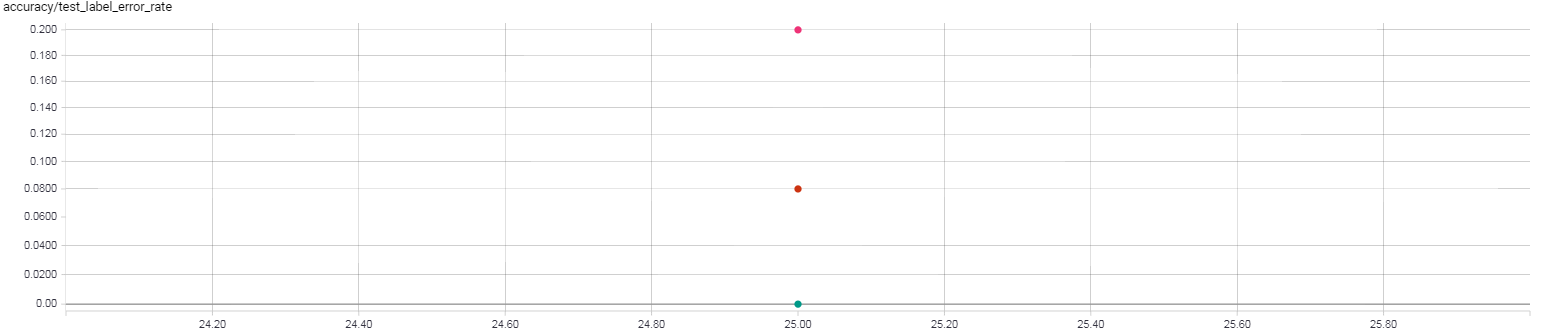
\includegraphics[width=\textwidth]		
	{model_development/3models_comparison/test_error_rate_3models}
	\caption{Test error rate.}
\end{figure}

\begin{table}[H]
\centering
	\caption{Test error rate results.}
	\begin{tabular}{| l | c | c | c |}
	\hline
	Models & Value & Epoch & Duration \\
	\hline
	Model1 -\tikzcircle[pink, fill=pink]{3pt}- &
	0.200 & 25.00 & 0s\\
	\hline
	Model2 -\tikzcircle[red, fill=red]{3pt}- &
	0.080 & 25.00 & 0s\\
	\hline
	Model3 -\tikzcircle[turquoise, fill=turquoise]{3pt}- &
	0.000 & 25.00 & 0s\\
	\hline
	\end{tabular}
\end{table}

\begin{figure}[H]
	\centering
	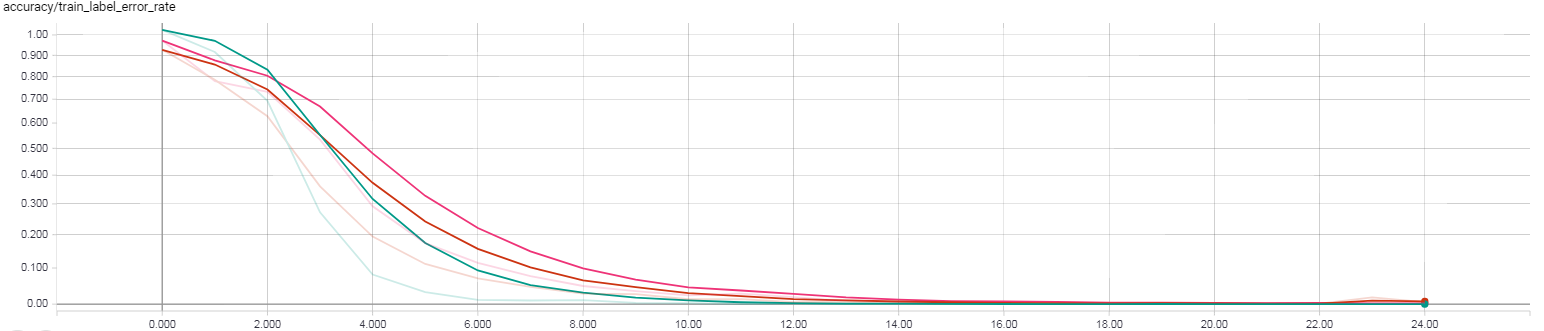
\includegraphics[width=\textwidth]		
	{model_development/3models_comparison/train_error_rate_3models}
	\caption{Training error rate.}
\end{figure}

\begin{table}[H]
\centering
	\caption{Training error rate results.}
	\begin{tabular}{| l | c | c | c |}
	\hline
	Models & Value & Epoch & Duration \\
	\hline
	Model1 -\tikzcircle[pink, fill=pink]{3pt}- &
	2.0887e-3 & 24.00 & 7m 46s\\
	\hline
	Model2 -\tikzcircle[red, fill=red]{3pt}- &
	5.1642e-3 & 24.00 & 9m 47s\\
	\hline
	Model3 -\tikzcircle[turquoise, fill=turquoise]{3pt}- &
	0.000 & 24.00 & 12m 50s\\
	\hline
	\end{tabular}
\end{table}

\begin{figure}[H]
	\centering
	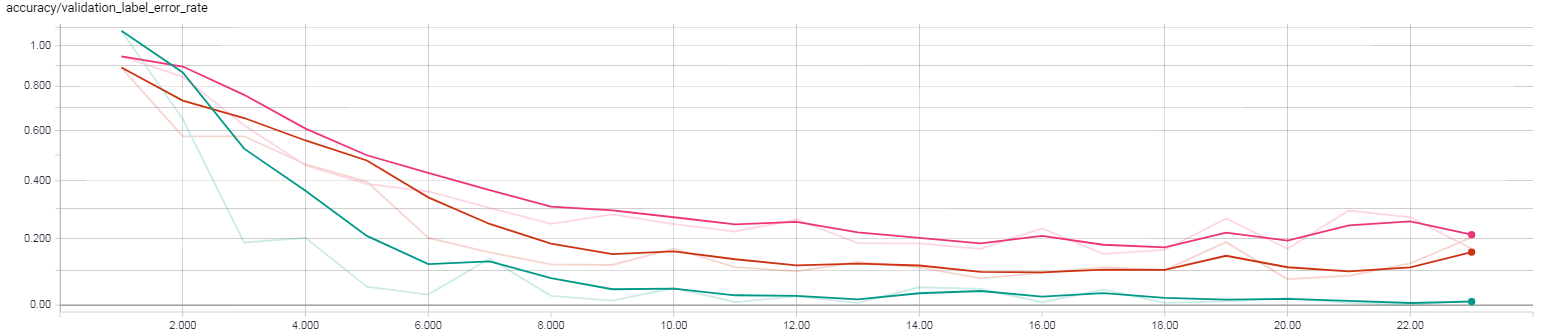
\includegraphics[width=\textwidth]		
	{model_development/3models_comparison/validation_error_rate_3models}
	\caption{Validation error rate.}
\end{figure}

\begin{table}[H]
\centering
	\caption{Validation error rate results.}
	\begin{tabular}{| l | c | c | c |}
	\hline
	Models & Value & Epoch & Duration \\
	\hline
	Model1 -\tikzcircle[pink, fill=pink]{3pt}- &
	0.1669 & 23.00 & 7m 9s\\
	\hline
	Model2 -\tikzcircle[red, fill=red]{3pt}- &
	0.2030 & 23.00 & 9m 8s\\
	\hline
	Model3 -\tikzcircle[turquoise, fill=turquoise]{3pt}- &
	0.01398 & 23.00 & 11m 49s\\
	\hline
	\end{tabular}
\end{table}

\begin{figure}[H]
	\centering
	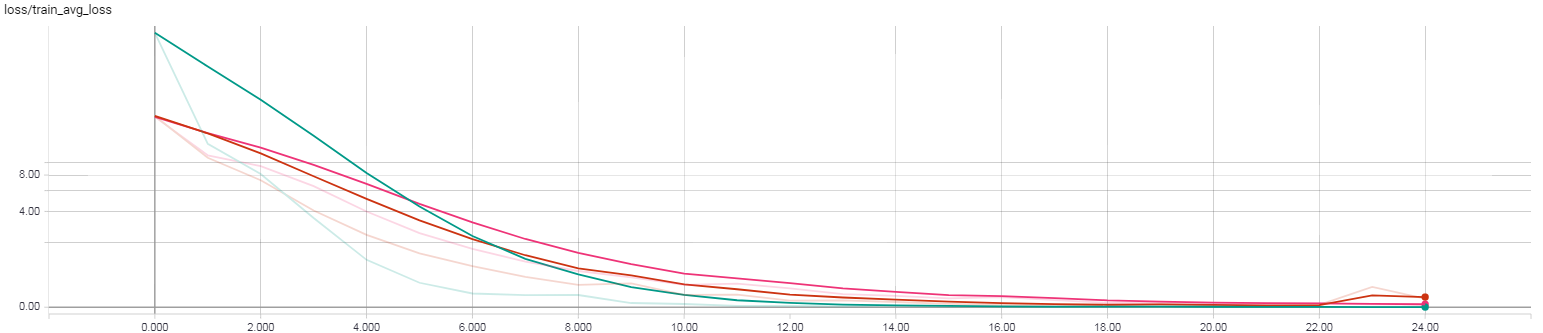
\includegraphics[width=\textwidth]		
	{model_development/3models_comparison/train_avg_loss_3models}
	\caption{Training average loss.}
\end{figure}

\begin{table}[H]
\centering
	\caption{Training average loss results.}
	\begin{tabular}{| l | c | c | c |}
	\hline
	Models & Value & Epoch & Duration \\
	\hline
	Model1 -\tikzcircle[pink, fill=pink]{3pt}- &
	0.04573 & 24.00 & 7m 46s\\
	\hline
	Model2 -\tikzcircle[red, fill=red]{3pt}- &
	0.1608 & 24.00 & 9m 47s\\
	\hline
	Model3 -\tikzcircle[turquoise, fill=turquoise]{3pt}- &
	1.2939e-3 & 24.00 & 12m 50s\\
	\hline
	\end{tabular}
\end{table}

\begin{figure}[H]
	\centering
	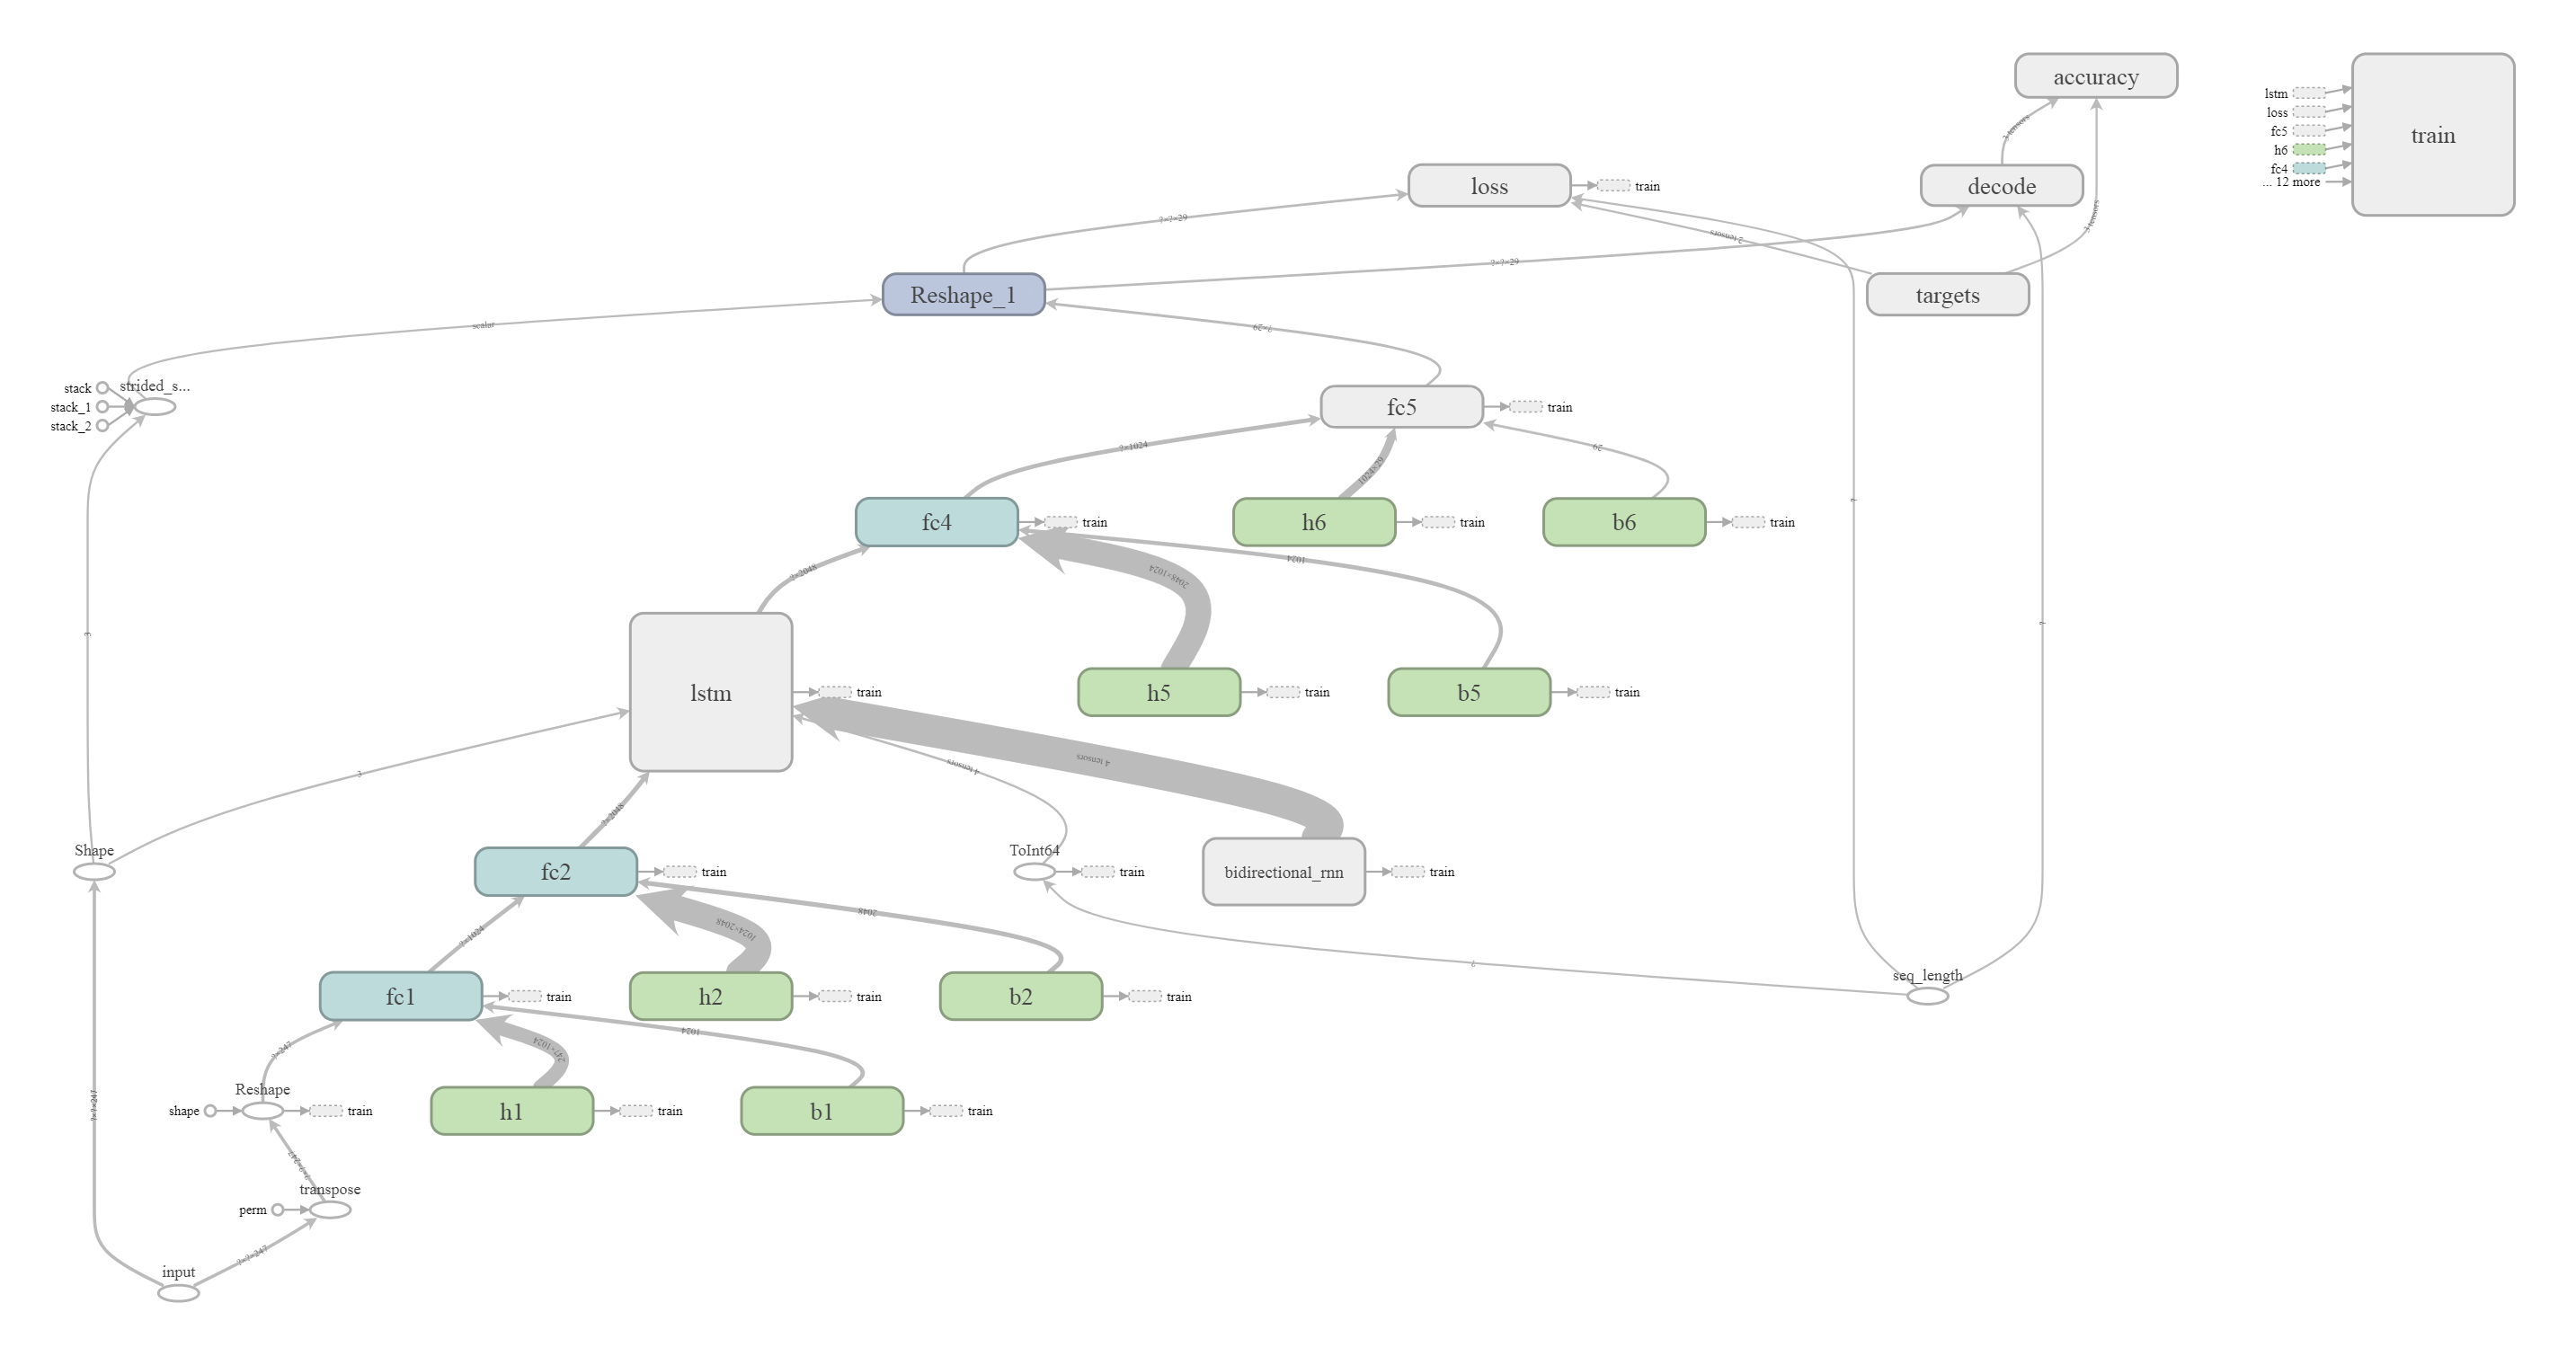
\includegraphics[width=\textwidth]		
	{model_development/birnn_v2_graph}
	\caption{Our BiRNN model graph.}
\end{figure}
	\chapter{Model Development Comparison Data}\label{ch:appDlabel}


\begin{table}[H]
\centering
	\caption{Models.}
	\begin{tabular}{ l  c }
	Model1 -\tikzcircle[pink, fill=pink]{3pt}- &
	(Their simpleLSTM Model)\\
	Model2 -\tikzcircle[red, fill=red]{3pt}- &
	(Our simpleLSTM Model)\\
	Model3 -\tikzcircle[turquoise, fill=turquoise]{3pt}- &
	(Our BiRNN Model)\\
	\end{tabular}
	\label{tab:3_models}
\end{table}


\begin{table}[H]
\centering
    \caption{Parameter values of the three model.}
    \begin{tabular}{| l | c | c | c | c |} 
    \hline
        Parameters & 
        Model1 -\tikzcircle[pink, fill=pink]{3pt}- &
        Model2 -\tikzcircle[red, fill=red]{3pt}- &
        Model3 -\tikzcircle[turquoise, fill=turquoise]{3pt}-\\
    \hline
        Batch Size & 
        50 \hfill 20 \hfill 20 & 
        50 \hfill 20 \hfill 20 & 
        50 \hfill 20 \hfill 20 \\
    \hline
        Dropout & 
        0.05 & 0.05 & 0.05 \\
    \hline
        Learning Rate & 
        0.001 & 0.001 & 0.001 \\ 
    \hline
    \end{tabular}
    \label{tab:3models_tab}
\end{table}

\begin{figure}[H]
	\centering
	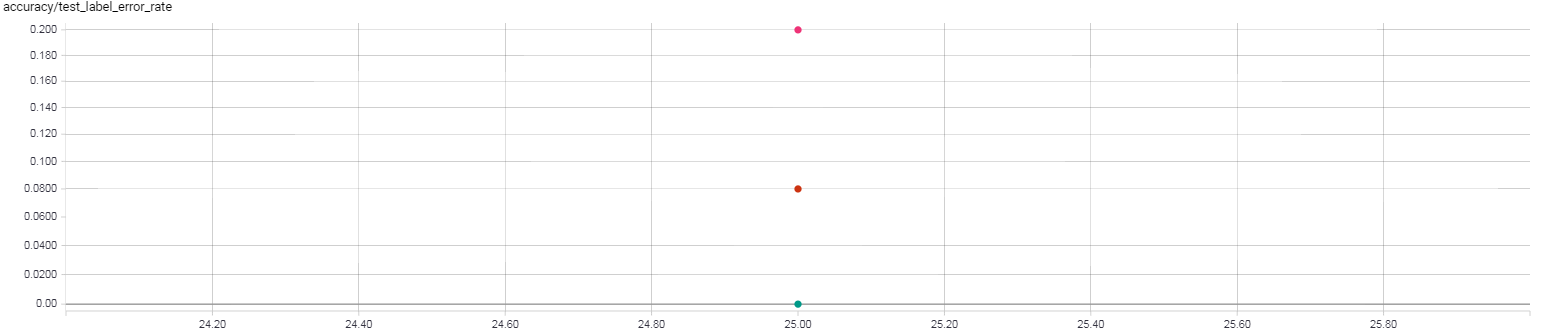
\includegraphics[width=\textwidth]		
	{model_development/3models_comparison/test_error_rate_3models}
	\caption{Test error rate.}
\end{figure}

\begin{table}[H]
\centering
	\caption{Test error rate results.}
	\begin{tabular}{| l | c | c | c |}
	\hline
	Models & Value & Epoch & Duration \\
	\hline
	Model1 -\tikzcircle[pink, fill=pink]{3pt}- &
	0.200 & 25.00 & 0s\\
	\hline
	Model2 -\tikzcircle[red, fill=red]{3pt}- &
	0.080 & 25.00 & 0s\\
	\hline
	Model3 -\tikzcircle[turquoise, fill=turquoise]{3pt}- &
	0.000 & 25.00 & 0s\\
	\hline
	\end{tabular}
\end{table}

\begin{figure}[H]
	\centering
	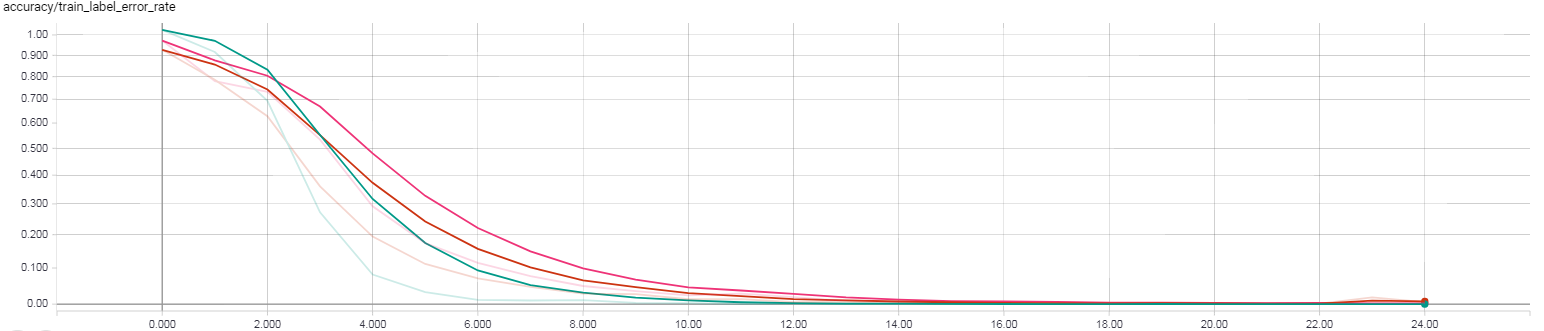
\includegraphics[width=\textwidth]		
	{model_development/3models_comparison/train_error_rate_3models}
	\caption{Training error rate.}
\end{figure}

\begin{table}[H]
\centering
	\caption{Training error rate results.}
	\begin{tabular}{| l | c | c | c |}
	\hline
	Models & Value & Epoch & Duration \\
	\hline
	Model1 -\tikzcircle[pink, fill=pink]{3pt}- &
	2.0887e-3 & 24.00 & 7m 46s\\
	\hline
	Model2 -\tikzcircle[red, fill=red]{3pt}- &
	5.1642e-3 & 24.00 & 9m 47s\\
	\hline
	Model3 -\tikzcircle[turquoise, fill=turquoise]{3pt}- &
	0.000 & 24.00 & 12m 50s\\
	\hline
	\end{tabular}
\end{table}

\begin{figure}[H]
	\centering
	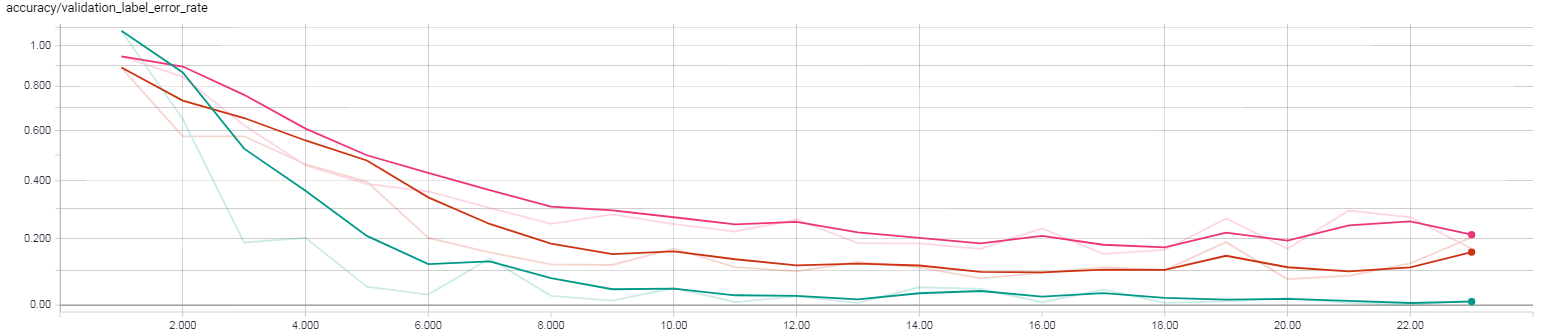
\includegraphics[width=\textwidth]		
	{model_development/3models_comparison/validation_error_rate_3models}
	\caption{Validation error rate.}
\end{figure}

\begin{table}[H]
\centering
	\caption{Validation error rate results.}
	\begin{tabular}{| l | c | c | c |}
	\hline
	Models & Value & Epoch & Duration \\
	\hline
	Model1 -\tikzcircle[pink, fill=pink]{3pt}- &
	0.1669 & 23.00 & 7m 9s\\
	\hline
	Model2 -\tikzcircle[red, fill=red]{3pt}- &
	0.2030 & 23.00 & 9m 8s\\
	\hline
	Model3 -\tikzcircle[turquoise, fill=turquoise]{3pt}- &
	0.01398 & 23.00 & 11m 49s\\
	\hline
	\end{tabular}
\end{table}

\begin{figure}[H]
	\centering
	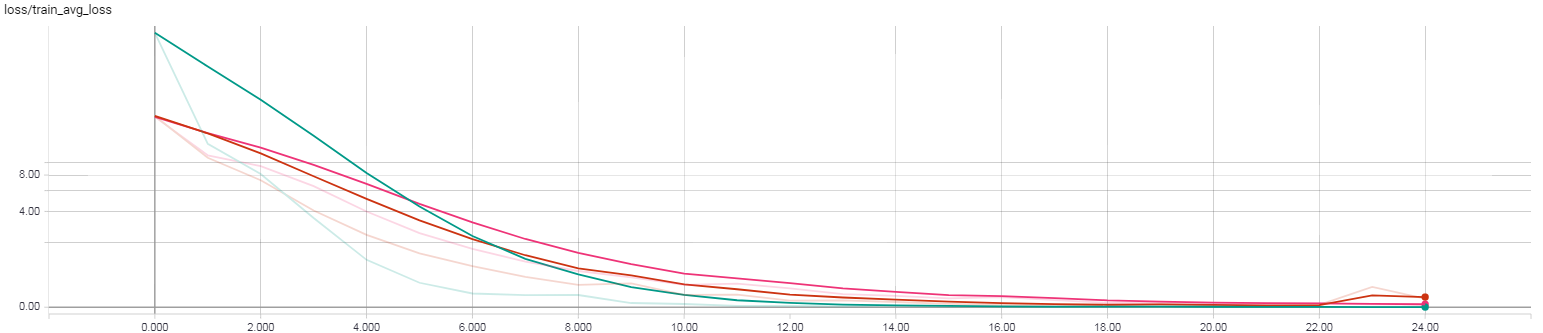
\includegraphics[width=\textwidth]		
	{model_development/3models_comparison/train_avg_loss_3models}
	\caption{Training average loss.}
\end{figure}

\begin{table}[H]
\centering
	\caption{Training average loss results.}
	\begin{tabular}{| l | c | c | c |}
	\hline
	Models & Value & Epoch & Duration \\
	\hline
	Model1 -\tikzcircle[pink, fill=pink]{3pt}- &
	0.04573 & 24.00 & 7m 46s\\
	\hline
	Model2 -\tikzcircle[red, fill=red]{3pt}- &
	0.1608 & 24.00 & 9m 47s\\
	\hline
	Model3 -\tikzcircle[turquoise, fill=turquoise]{3pt}- &
	1.2939e-3 & 24.00 & 12m 50s\\
	\hline
	\end{tabular}
\end{table}

\begin{figure}[H]
	\centering
	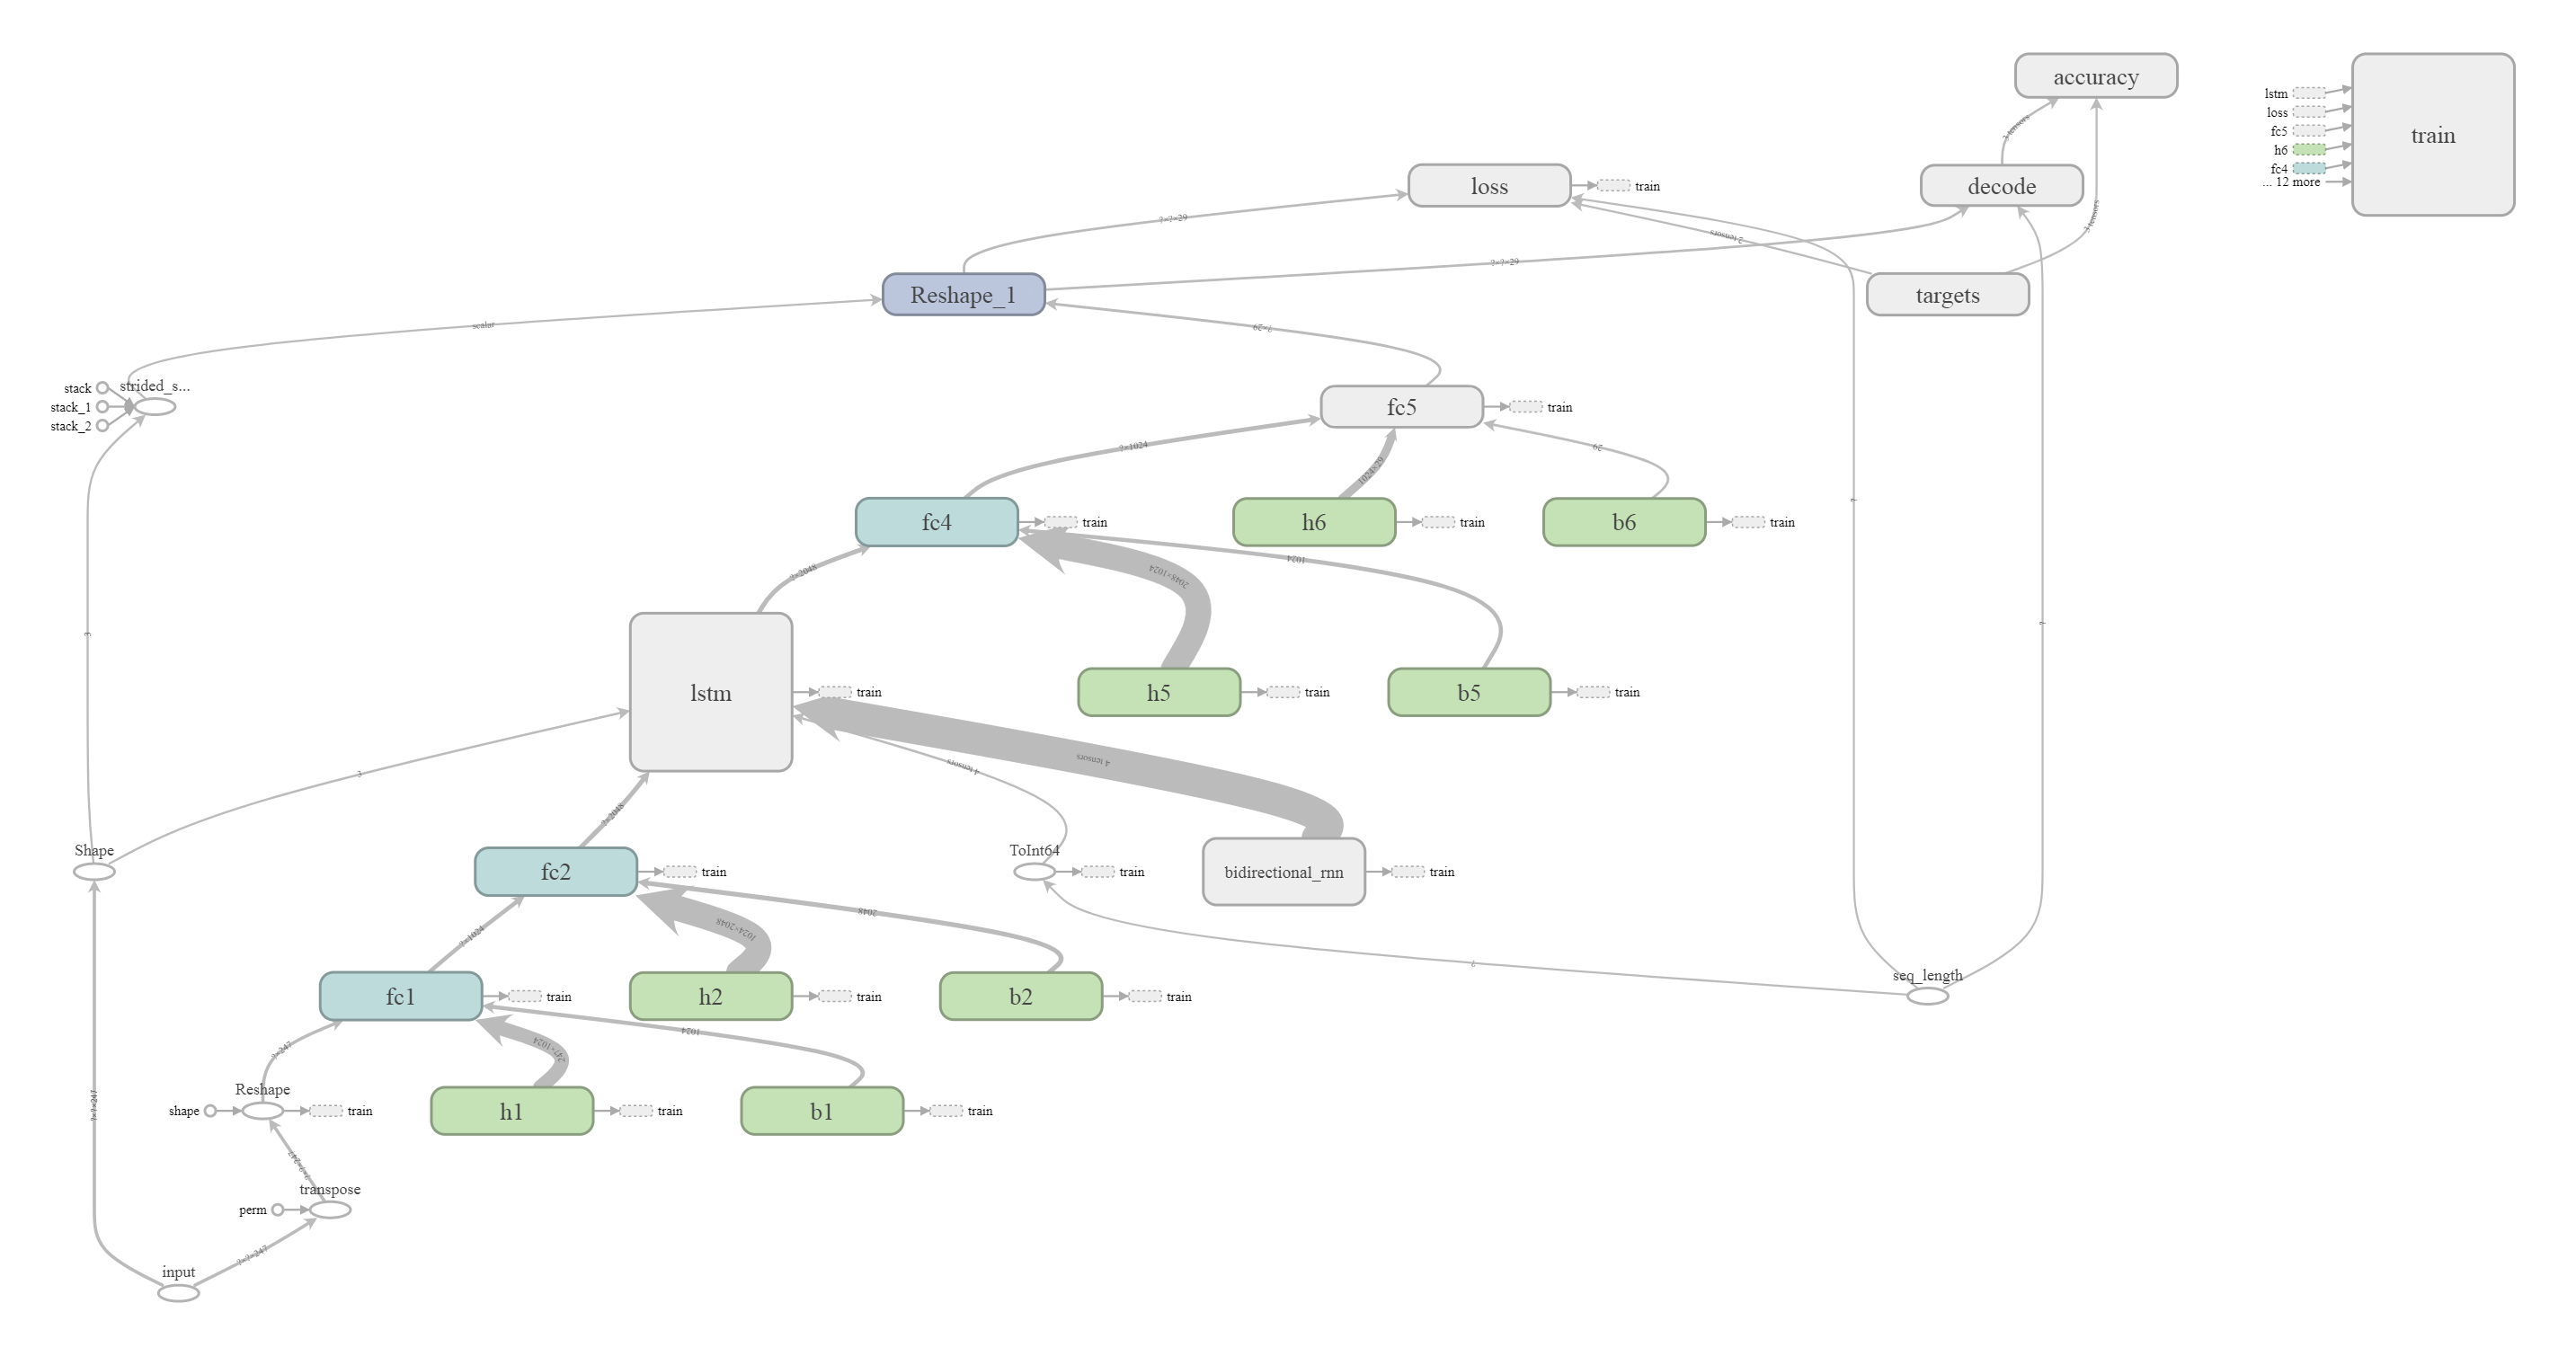
\includegraphics[width=\textwidth]		
	{model_development/birnn_v2_graph}
	\caption{Our BiRNN model graph.}
\end{figure}
	
\end{document}
%--------------------------------------------------------------%
